%\documentclass[14pt]{extarticle}
\documentclass[12pt, a4paper]{article}
\usepackage[russian]{babel}
\usepackage[utf8]{inputenc}
\usepackage[T2A]{fontenc}
\usepackage{amsfonts}
\usepackage{amsmath}
\usepackage[
left 	= 	30	mm,
right 	=	15	mm,
top 	=	20	mm,
bottom 	=	20	mm,
]{geometry}

\usepackage{indentfirst} % Красная строка

\setlength{\parindent}{1.25 cm}

\usepackage[toc,page]{appendix}

\renewcommand{\baselinestretch}{1.5}

\usepackage{titlesec}

\titleformat{\section}
{\normalfont\fontsize{14}{14}\bfseries}{\thesection}{1em}{}

\titleformat{\subsection}
{\normalfont\fontsize{14}{14}\bfseries}{\thesubsection}{1em}{}

\usepackage[intoc]{nomencl}
\renewcommand{\nomname}{Обозначения и сокращения}
\makenomenclature

%%% Математика

% Шрифты для математики
\usepackage{amsmath}
\usepackage{amsfonts}
\usepackage{amssymb}
\usepackage{cancel}
\usepackage{mathrsfs}
\usepackage{mathtools}
\usepackage{upgreek}
\usepackage{xfrac}


%%% Иллюстрации
\usepackage{graphicx}
\usepackage{subcaption}
\usepackage{wrapfig}
\usepackage[export]{adjustbox}
%\graphicspath{{./img/}}

\makeatletter % список литературы
\def\@biblabel#1{#1. }
\makeatother

% Графики
\usepackage{pgfplots}
\pgfplotsset{compat=1.3}
\usepgfplotslibrary{patchplots}
%\usepackage{patchplots}
\pgfplotsset{	width	=	14	cm,
	x label style={
		font = {\small\sffamily},
		yshift = 1mm
	},
	tick label style={
		font = {\scriptsize},
	},
	y label style={
		font = {\small\sffamily},
		yshift = -1mm,
		at={(ticklabel cs:0.5)},
		%      					rotate=90,
		anchor=near ticklabel
	},
	every tick/.style	=	{
		black, 
		line width 	= 	.5	pt
	},
	axis line style 	= 	{
		line width 	= 	.5	pt
	},
	grid style	=	{
		gray,
		dotted
	},
	minor x tick num = 1,
	minor y tick num = 1,
	no markers,
	grid = major,
	every axis/.append style	=	{
		line width	=	.7	pt
	}
}

%Подписи
\usepackage		[margin		= 10	pt,
%					font		= footnotesize, 
%labelfont	= bf, 
labelsep	= endash, 
%labelfont	= bf,
%					textfont	= sl,
margin		= 0 	pt,  
aboveskip 	= 4		pt, 
belowskip 	= -6	pt,
figurename= Рисунок] {caption}
\usepackage		[margin		= 10	pt,
font		= footnotesize, 
labelfont	= bf, 
labelsep	= endash, 
labelfont	= bf,
textfont	= sl,
margin		= 0 	pt,  
aboveskip 	= 4		pt, 
belowskip 	= 6	pt]	{subcaption}

\makeatletter
%\newcounter{figure}[section]
%\newcounter{table}[section]
\renewcommand{\thefigure}{\thesection.\@arabic\c@figure}
\renewcommand{\thetable}{\thesection.\@arabic\c@table}
\makeatother


%%% Insert pdf pages
\usepackage[final]{pdfpages}


%%% Color highlight
\usepackage{xcolor}

% Ссылки внутри текста
\usepackage{hyperref}

\begin{document}
	\counterwithin{lstlisting}{section}
%	\includepdf[pages=-]{titlesheet.pdf}
	
\includepdf[pages=1]{title.pdf}
	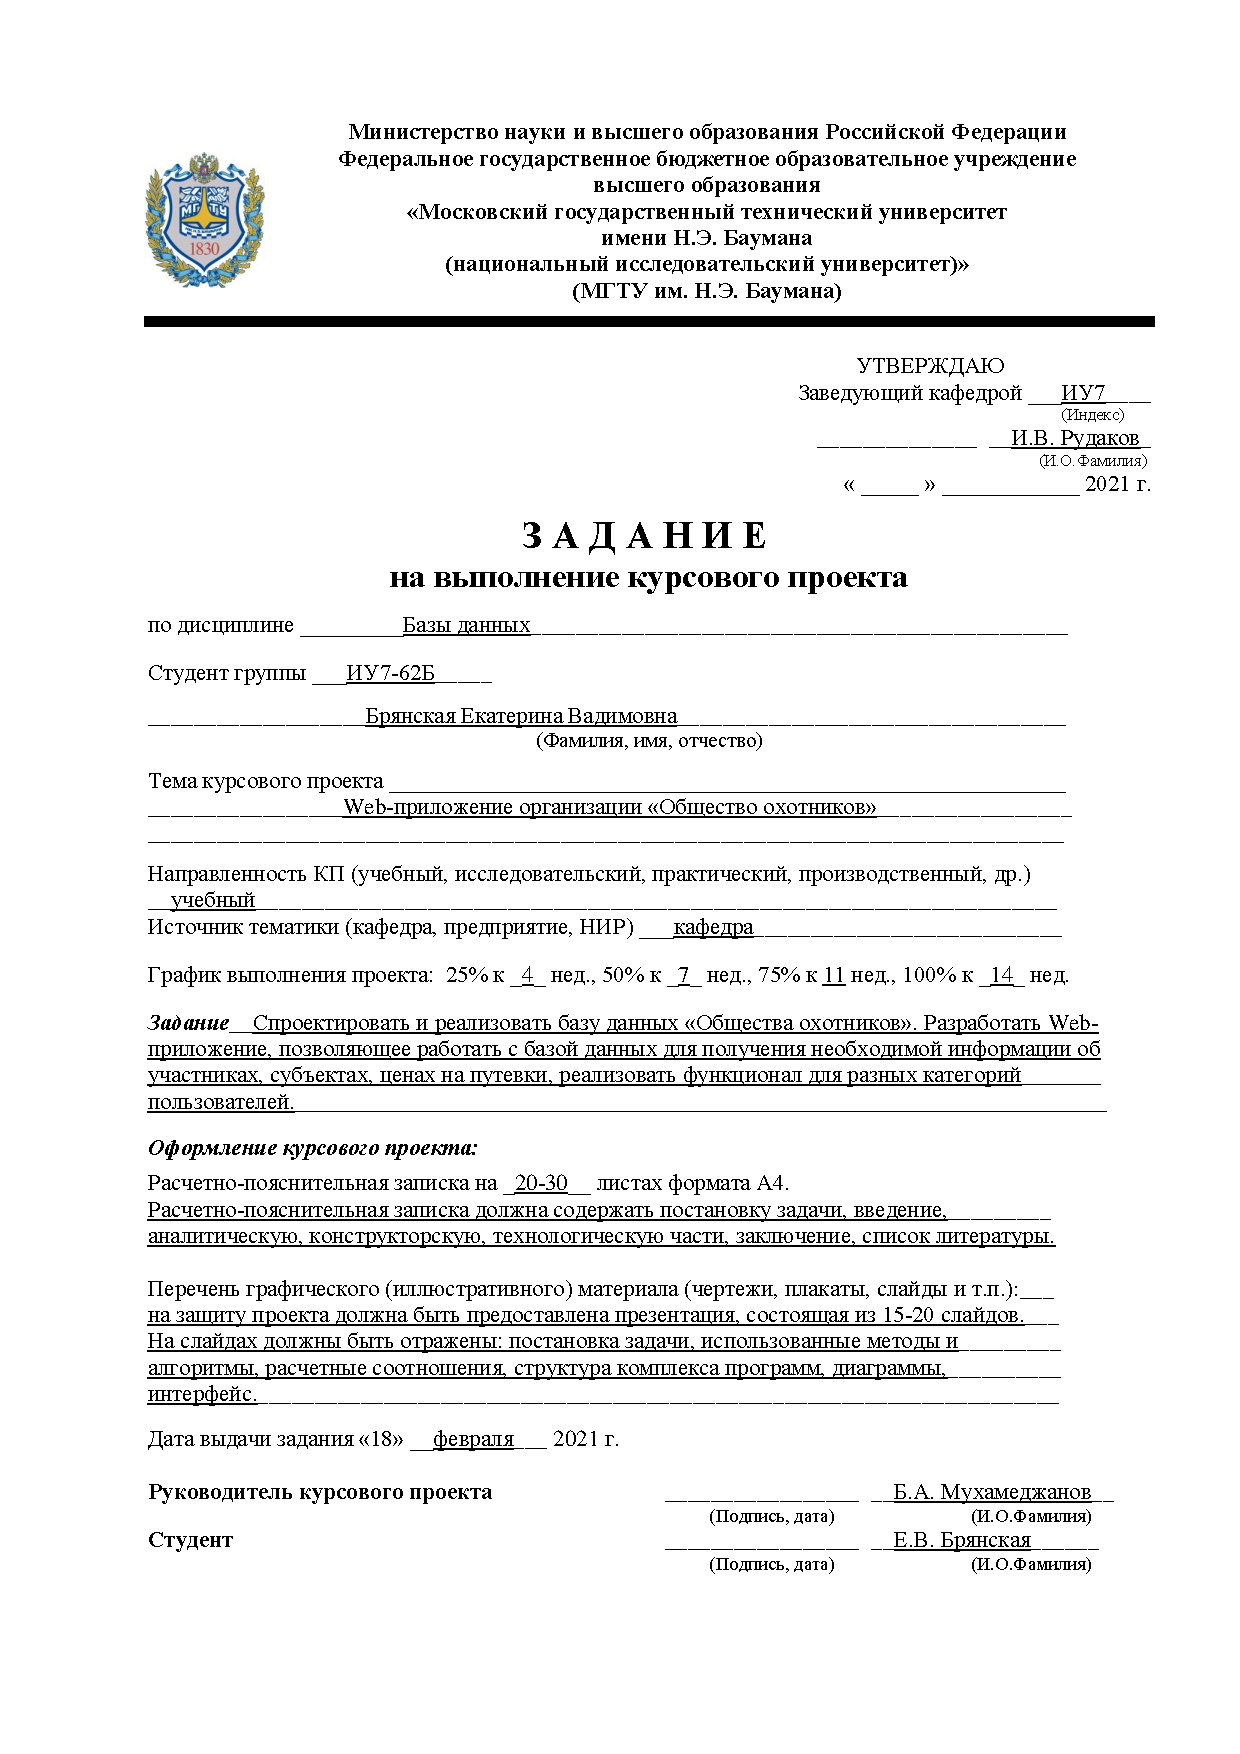
\includepdf[pages=1]{task.pdf}
	
	\setcounter{page}{3}
	
	\section*{Реферат}
рит пи тп
	\newpage
	
	% Содержание
	\tableofcontents
	\newpage
	
%	\printnomenclature[2em]
%	В тексте писать так: $\beta$\nomenclature{$\beta$}{Вторая буква греческого алфавита}
	
	\section*{Введение}
	\addcontentsline{toc}{section}{Введение}
	
	В настоящее время процент использования информационных технологий в различных сферах растёт с каждым годом, так, согласно исследованиям \cite{Russia-in-numbers} за 2018 год он вырос на $3\%$ по сравнению с предыдущим, и такая тенденция сохраняется на протяжении нескольких лет.\\

	На сегодняшний день использование такого рода технологий позволяет любой организации без препятствий взаимодействовать с большими потоками информации. Быстрый доступ к базам данных обеспечивает оперативность обмена материалами и согласованность всей работы в целом. \\
	
	Однако внедрение подобного подхода в различные инфраструктуры происходит не равномерно, например, в Распоряжении Правительства РФ "Об утверждении Стратегии развития охотничьего хозяйства в Российской Федерации до 2030 года" \cite{doc_problems} рассматривается проблема использования консервативных и неэффективных методов работы, которые затрудняют организацию и контроль. \\
	
	Объектом разработки курсового проекта было выбрано <<Общество охотников>>, осуществляющее возможность подачи заявки и покупки путёвок. \\
	
	\textbf{Целью} работы - спроектировать и реализовать базу данных для <<Общества охотников>>, и разработать Web-приложение для взаимодействия с базой данных.\\
	Выделены следующие \textbf{задачи}:
	\begin{enumerate}
		\item[1)] провести анализ существующих решений;
		\item[2)] формализовать задание и определить необходимый функционал;
		\item[3)] осуществить обзор существующих решений;
		\item[4)] провести анализ существующих СУБД;
		\item[5)] спроектировать базу данных для хранения и структурирования данных;
		\item[6)] реализовать спроектированную базу данных с использованием выбранной СУБД;
		\item[7)] разработать соответствующее Web-приложение.
	\end{enumerate}
	  
	\newpage
	
	\section{Аналитическая часть}	
	\subsection{Обзор существующих аналогов}
	В настоящий момент существует несколько сервисов, выполняющих похожие задачи.
	
	\subsubsection{Геопортал охотничьего хозяйства России}
	Этот портал предоставляет удобный сервис для наилучшего ориентирования пользователей среди разнообразных охотничьих хозяйств. Он включает в себя набор интерактивных карт субъектов Российской Федерации с возможностью перехода по клику на информационную страницу, соответствующую выбранному элементу. \cite{maps} \\
	
	Однако набор действий на сайте очень ограничен. Так, ссылки, указывающие на возможность приобретения путёвки на охоту, перенаправляют пользователя либо на инструкцию, в которой указано, какое учреждение нужно очно посетить для оформления соответствующих документов, либо на сайт с уже устаревшей информацией. И лишь некоторые субъекты перенаправляют на сайт Госуслуг для подачи заявки онлайн. Личного кабинета у пользователя на этом портале нет. \\
	
	\subsubsection{Портал государственных и муниципальных услуг}
	Сервис поддерживает подачу заявок онлайн, для этого необходимо заполнить формы и подгрузить необходимые документы. Но также обязательным условием является посещение МФЦ. Все оформленные путёвки появляются в специально отведённом разделе в личном кабинете.\\
	
	Основным неудобством в работе данных сервисов является отсутствие возможности оформления документов на охоту удалённо, в любом случае, требуется посещение специального учреждения. Также ввиду ограниченного функционала личный кабинет либо отсутствует, либо предоставляет только общую информацию, за детальным разъяснением приходится обращаться в сторонние сервисы. Поэтому в качестве одной из задач данной работы ставится выполнение указанных требований.
	
	\subsection{Формализация задачи}
	В ходе выполнения курсовой работы должно быть спроектировано и реализовано Web-приложение, предоставляющее интерфейс для работы с данными о членах организации, путёвках, прайс-листах для различных категорий пользователей (таких как, администратор, егерь, охотник). Для каждого участника должен быть определён свой набор прав и разрешённых действий.\\
	
	Кроме того, необходимо обеспечить возможность регистрации с дальнейшим подтверждением со стороны администратора. В случае положительного ответа пользователю предоставляется функционал в соответствии с его категорией.
	
	\subsection{Формализация ролей}
	Было выделено три категории пользователей.\\
	
	\textbf{Охотник} \\
		Может выполнять следующие действия.
		\begin{itemize}
			\item Просматривать:
			\begin{itemize}
				\item личную информацию;
				\item контакты всех егерей занесённых в базу данных;
				\item свои одобренные путёвки и заявки на их покупку;
				\item прайс-лист по всем хозяйствам и секторам с возможностью поиска необходимого субъекта.
			\end{itemize}
			\item Отправлять:
			\begin{itemize} 
			 	\item заявки на путёвки с указанием места охоты и количества животных.
			\end{itemize}
		 	\item Отзывать:
		 	\begin{itemize}
		 		\item созданную ранее заявку.
		 	\end{itemize}
		\end{itemize}
	
		\textbf{Егерь} \\
		Ему предоставляются следующие возможности.
		\begin{itemize}
			\item Просматривать:
			\begin{itemize}
				\item личную информацию;
				\item общую информацию о всех охотниках с возможностью поиска по ФИО и номеру охотничьего билета;
				\item контакты всех егерей занесённых в базу данных;
				\item прайс-лист закреплённого за ним сектора с возможностью поиска необходимого животного;
				\item заявки на охоту, а также одобренные путёвки в его сектор.
			\end{itemize}
			\item Отклонить или принять:
			\begin{itemize} 
				\item заявку на путёвку в его сектор.
			\end{itemize}
			\item Оформить:
			\begin{itemize} 
				\item новую путёвку в закреплённый за ним сектор с указанием номера билета охотника и позиции из доступного прайс-листа.
			\end{itemize}
			\item Закрыть:
			\begin{itemize}
				\item уже одобренную путёвку.
			\end{itemize}
			
		\end{itemize}
		
		\textbf{Администратор}\\
		Для него определён соответствующий набор действий.
		\begin{itemize}
			\item Просматривать:
			\begin{itemize}
				\item личную информацию;
				\item информацию о всех охотниках, занесённых в базу данных, с возможностью поиска по ФИО и номеру билета;
				\item информацию о всех егерях, занесённых в базу данных, с возможностью поиска по ФИО и субъекту;
				\item информацию о всех администраторах, занесённых в базу данных, с возможностью поиска по ФИО;
				\item заявки на охоту во всех возможных хозяйствах и секторах;
				\item заявки на регистрацию в качестве охотника, егеря, администратора;
				\item выданные путёвки во всех возможных хозяйствах и секторах.
			\end{itemize}
			\item Отклонить или принять:
			\begin{itemize} 
				\item заявку на охоту в любой субъект;
				\item заявку на регистрацию в качестве охотника, егеря, администратора.
			\end{itemize}
			\item Оформить:
			\begin{itemize} 
				\item новую путёвку с указанием названия хозяйства, номера сектора, номера билета охотника и позиции из доступного прайс-листа.
			\end{itemize} 
			\item Закрыть:
			\begin{itemize}
				\item уже одобренную путёвку из любого субъекта.
			\end{itemize}
			\item Удалить аккаунт:
			\begin{itemize} 
				\item охотника;
				\item егеря;
				\item администратора (кроме себя самого).
			\end{itemize}
		\end{itemize}
	
	\subsection{Формализация данных}
	На рисунке \ref{fig1:image} приведена ER-диаграмма схемы сущностей.
	
	\begin{figure}[ph!]
		\centering
		\begin{center}
			{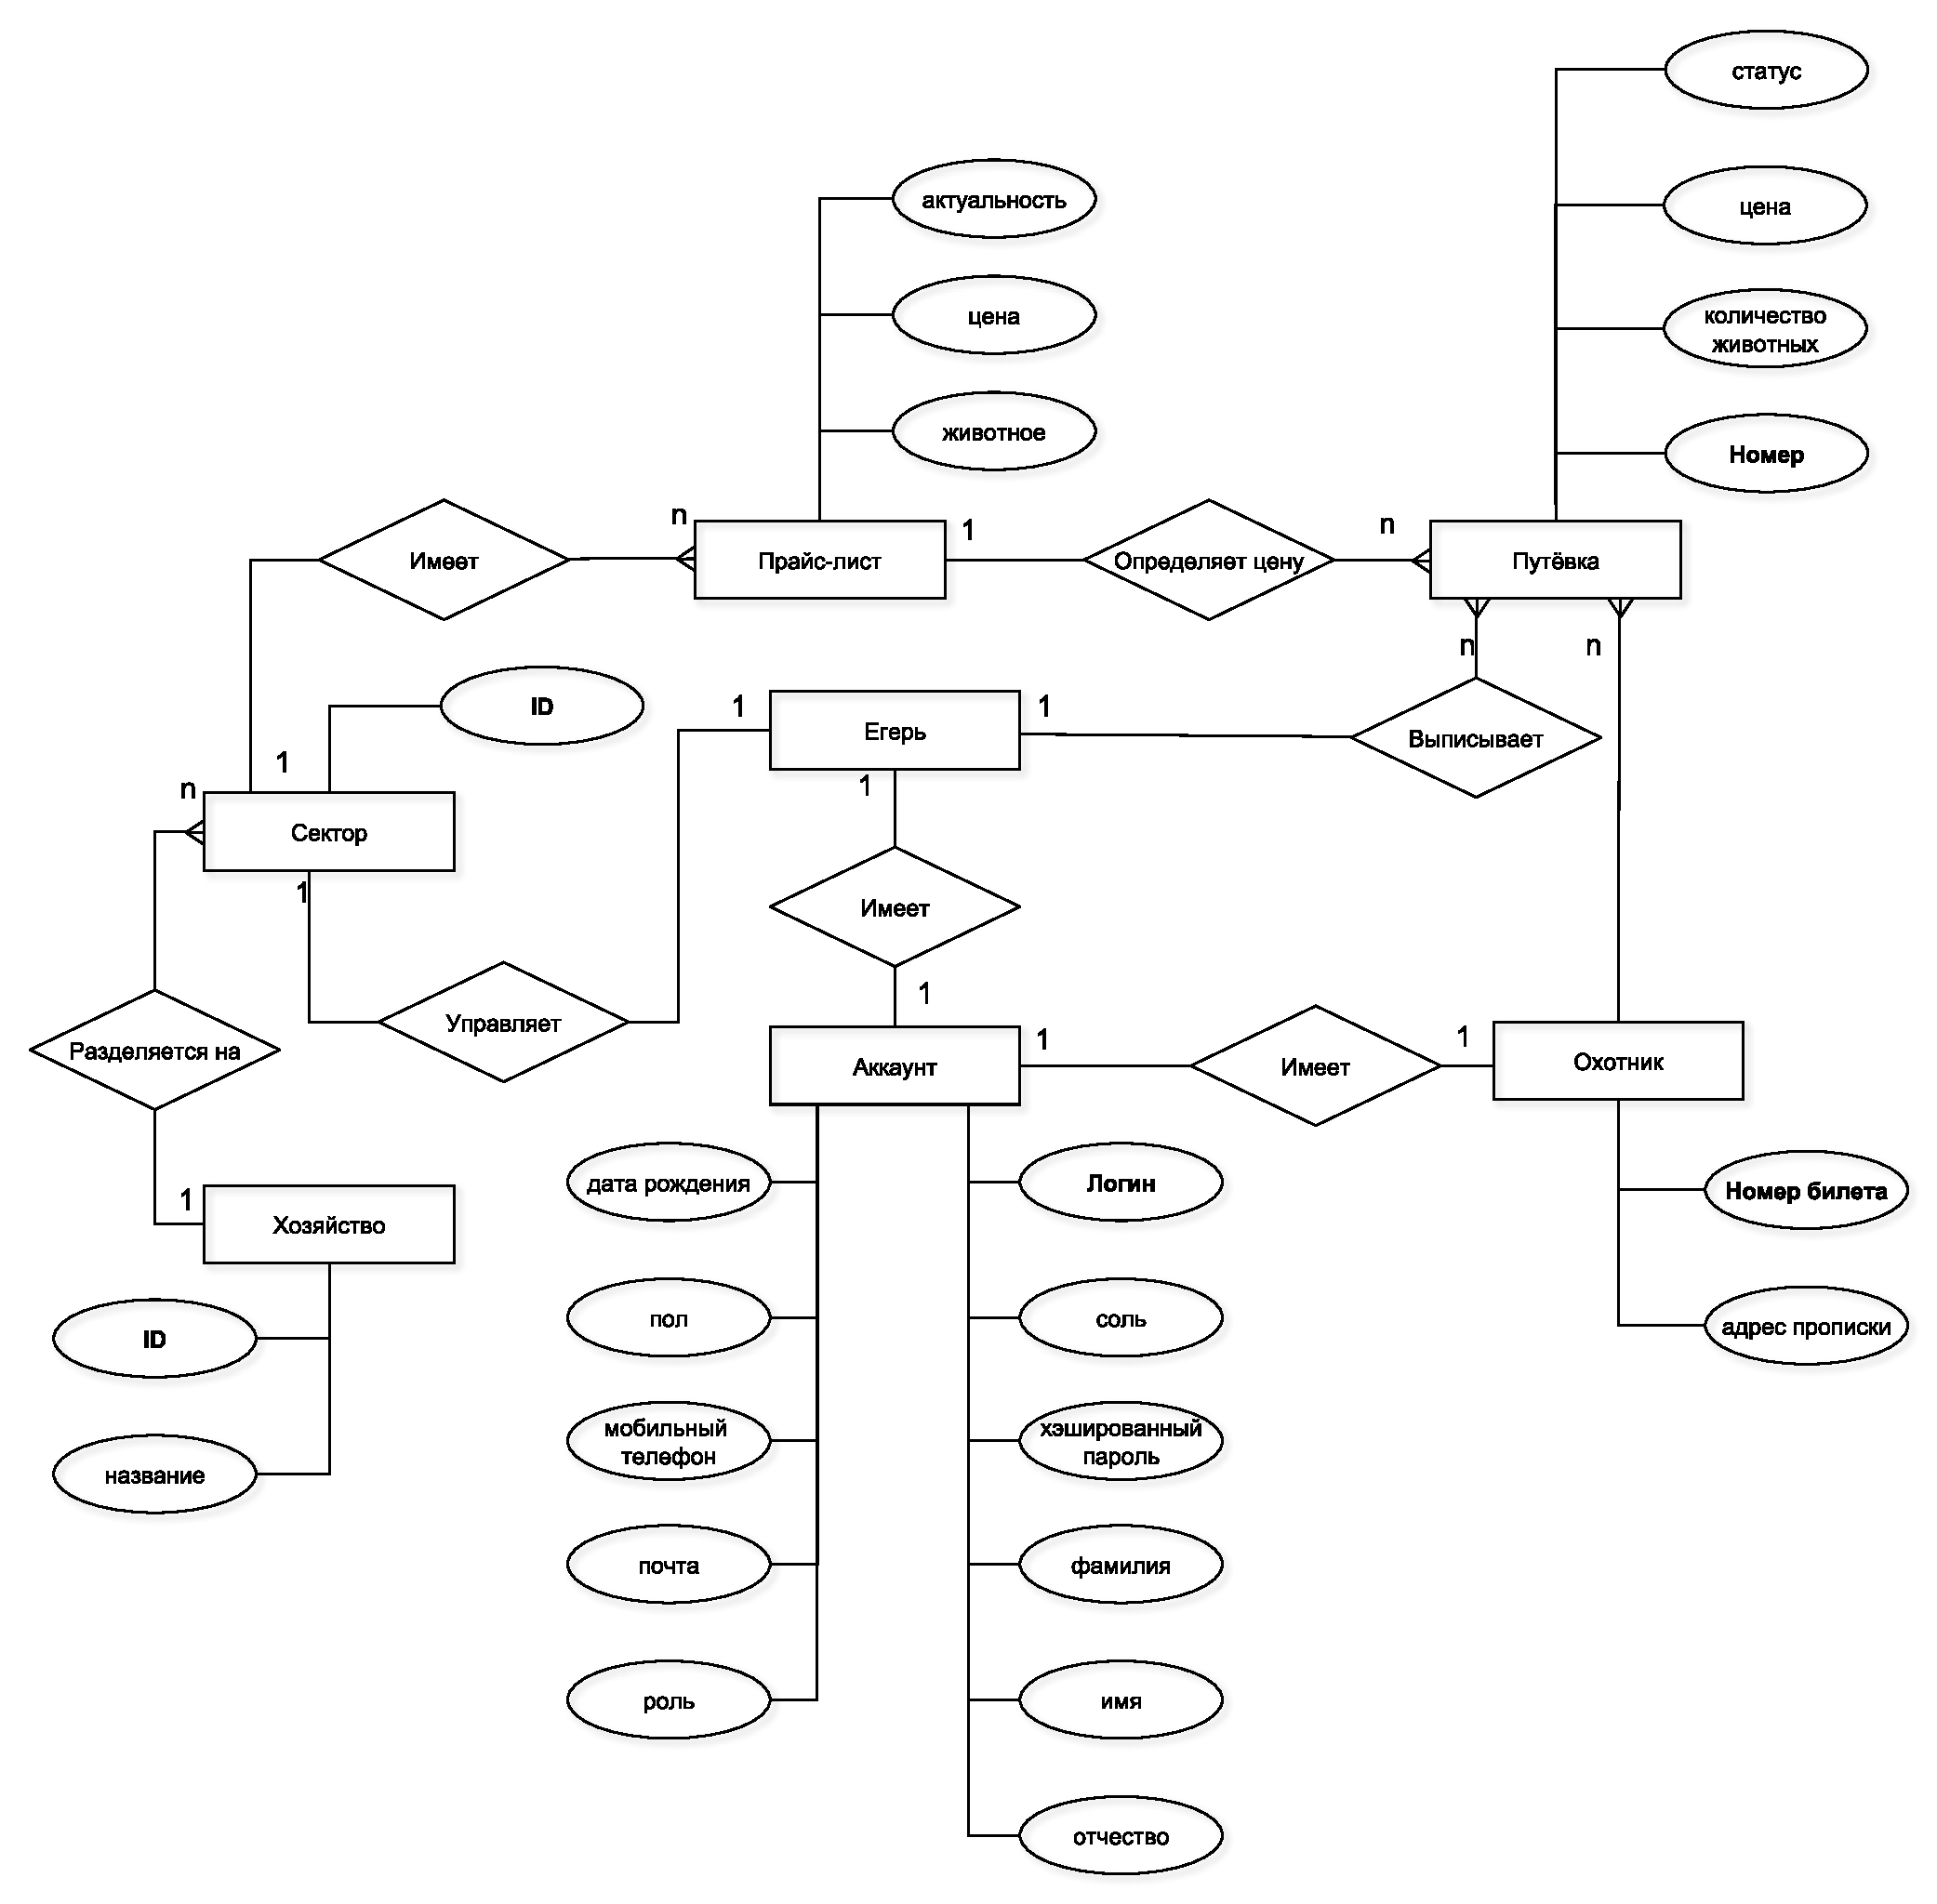
\includegraphics[scale=0.45]{schemes/er.pdf}}
			\caption{ER-диаграмма сущностей}
			\label{fig1:image}
		\end{center}
	\end{figure}

	\newpage

	\subsection{Базы данных}
	\subsubsection{Определение базы данных}
	\textbf{База данных (БД)} -  это самодокументированное собрание интегрированных записей.\\
	\textbf{Самодокументированная} - хранятся метаданные (данные о данных).\\
	\textbf{Интегрированные записи} – файлы данных.
	
	\subsubsection{Требования к БД}
	\begin{enumerate}
		\item[1)] Неизбыточность \\
		Не хранится лишняя информация.
		\item[2)] Эффективность доступа \\
		Малое время отклика на запрос.
		\item[3)] Совместное использование
		\item[4)] Безопасность
		\item[5)] Восстановление после сбоя
		\item[6)] Целостность \\
		Если есть ссылка на какой-то объект, то он должен быть. Нельзя ссылаться на несуществующие объекты.
		\item[7)] Независимость от сторонних приложений
	\end{enumerate}

	\subsubsection{Модели данных}
	\textbf{Модель данных} - это абстрактное, самодостаточное, логическое определение объектов, операторов и прочих элементов, в совокупности составляющих абстрактную машину доступа к данным, с которой взаимодействует пользователь. Эти объекты позволяют моделировать структуру данных, а операторы — поведение данных. \cite{db} \\
	
	Выделяют три основные модели данных.
	\begin{enumerate}
		\item[1)] Иерархическая \\
		Подразумевается, что элементы организованы в структуры, связанные между собой иерархическими или древовидными связями. Родитель может иметь несколько потомков. Но у потомка может быть только один предок.
		\item[2)] Сетевая \\
		У родителя также может быть несколько потомков, а у дочернего элемента — несколько предков.
		\item[3)] Реляционная \\
		Главное отличие состоит в том, что информация хранится в виде таблиц (отношений), состоящих из нескольких записей (кортежей), обладающих одним и тем же набором атрибутов, или полей. Используются чаще, чем две другие модели.
	\end{enumerate}

	Реляционная модель данных наиболее подходит для решения поставленной задачи, поскольку она более гибкая и удобная в использовании. Также она лучше всего соответствует описанным ранее отношениям между выделенными сущностями.
	
	\subsubsection{Система управления базами данных (СУБД)}
	\textbf{Система управления базами данных (СУБД)} - приложение, позволяющее создать базу данных и манипулировать данными (вставлять, обновлять, удалять и выбирать).\\
	Основные компоненты СУБД. \cite{db_systems}
	\begin{itemize}
		\item Ядро \\
		Отвечает за управление данными во внешней и оперативной памяти и журнализацию.
		\item Процессор языка БД\\
		Используется для оптимизации запросов на извлечение и изменение данных.
		\item Подсистема поддержки времени исполнения\\
		Интерпретирует программы манипуляции данными, создающие пользовательский интерфейс с СУБД.
		\item Сервисные программы\\
		Отвечают за обеспечение дополнительных возможностей.
	\end{itemize}

	\subsection*{Вывод}
	Был проведён обзор существующих решений, на основе анализа предоставляемых ими возможностей была формализована задача курсового проекта, также были определены категории пользователей и соответствующие им действия. Кроме того, приведены некоторые теоретические сведения, необходимые для дальнейшей работы.
	
	
	\newpage
	
	\setcounter{table}{0}
	\setcounter{figure}{0}
	\section{Конструкторская часть}	
	\subsection{Use-Case диаграмма}
	На рисунках \ref{fig2:image}-\ref{fig4:image} приведены диаграммы вариантов использования для каждого актора, полная схема находится в приложении.
	
	\begin{figure}[ph!]
		\centering
		\begin{center}
			{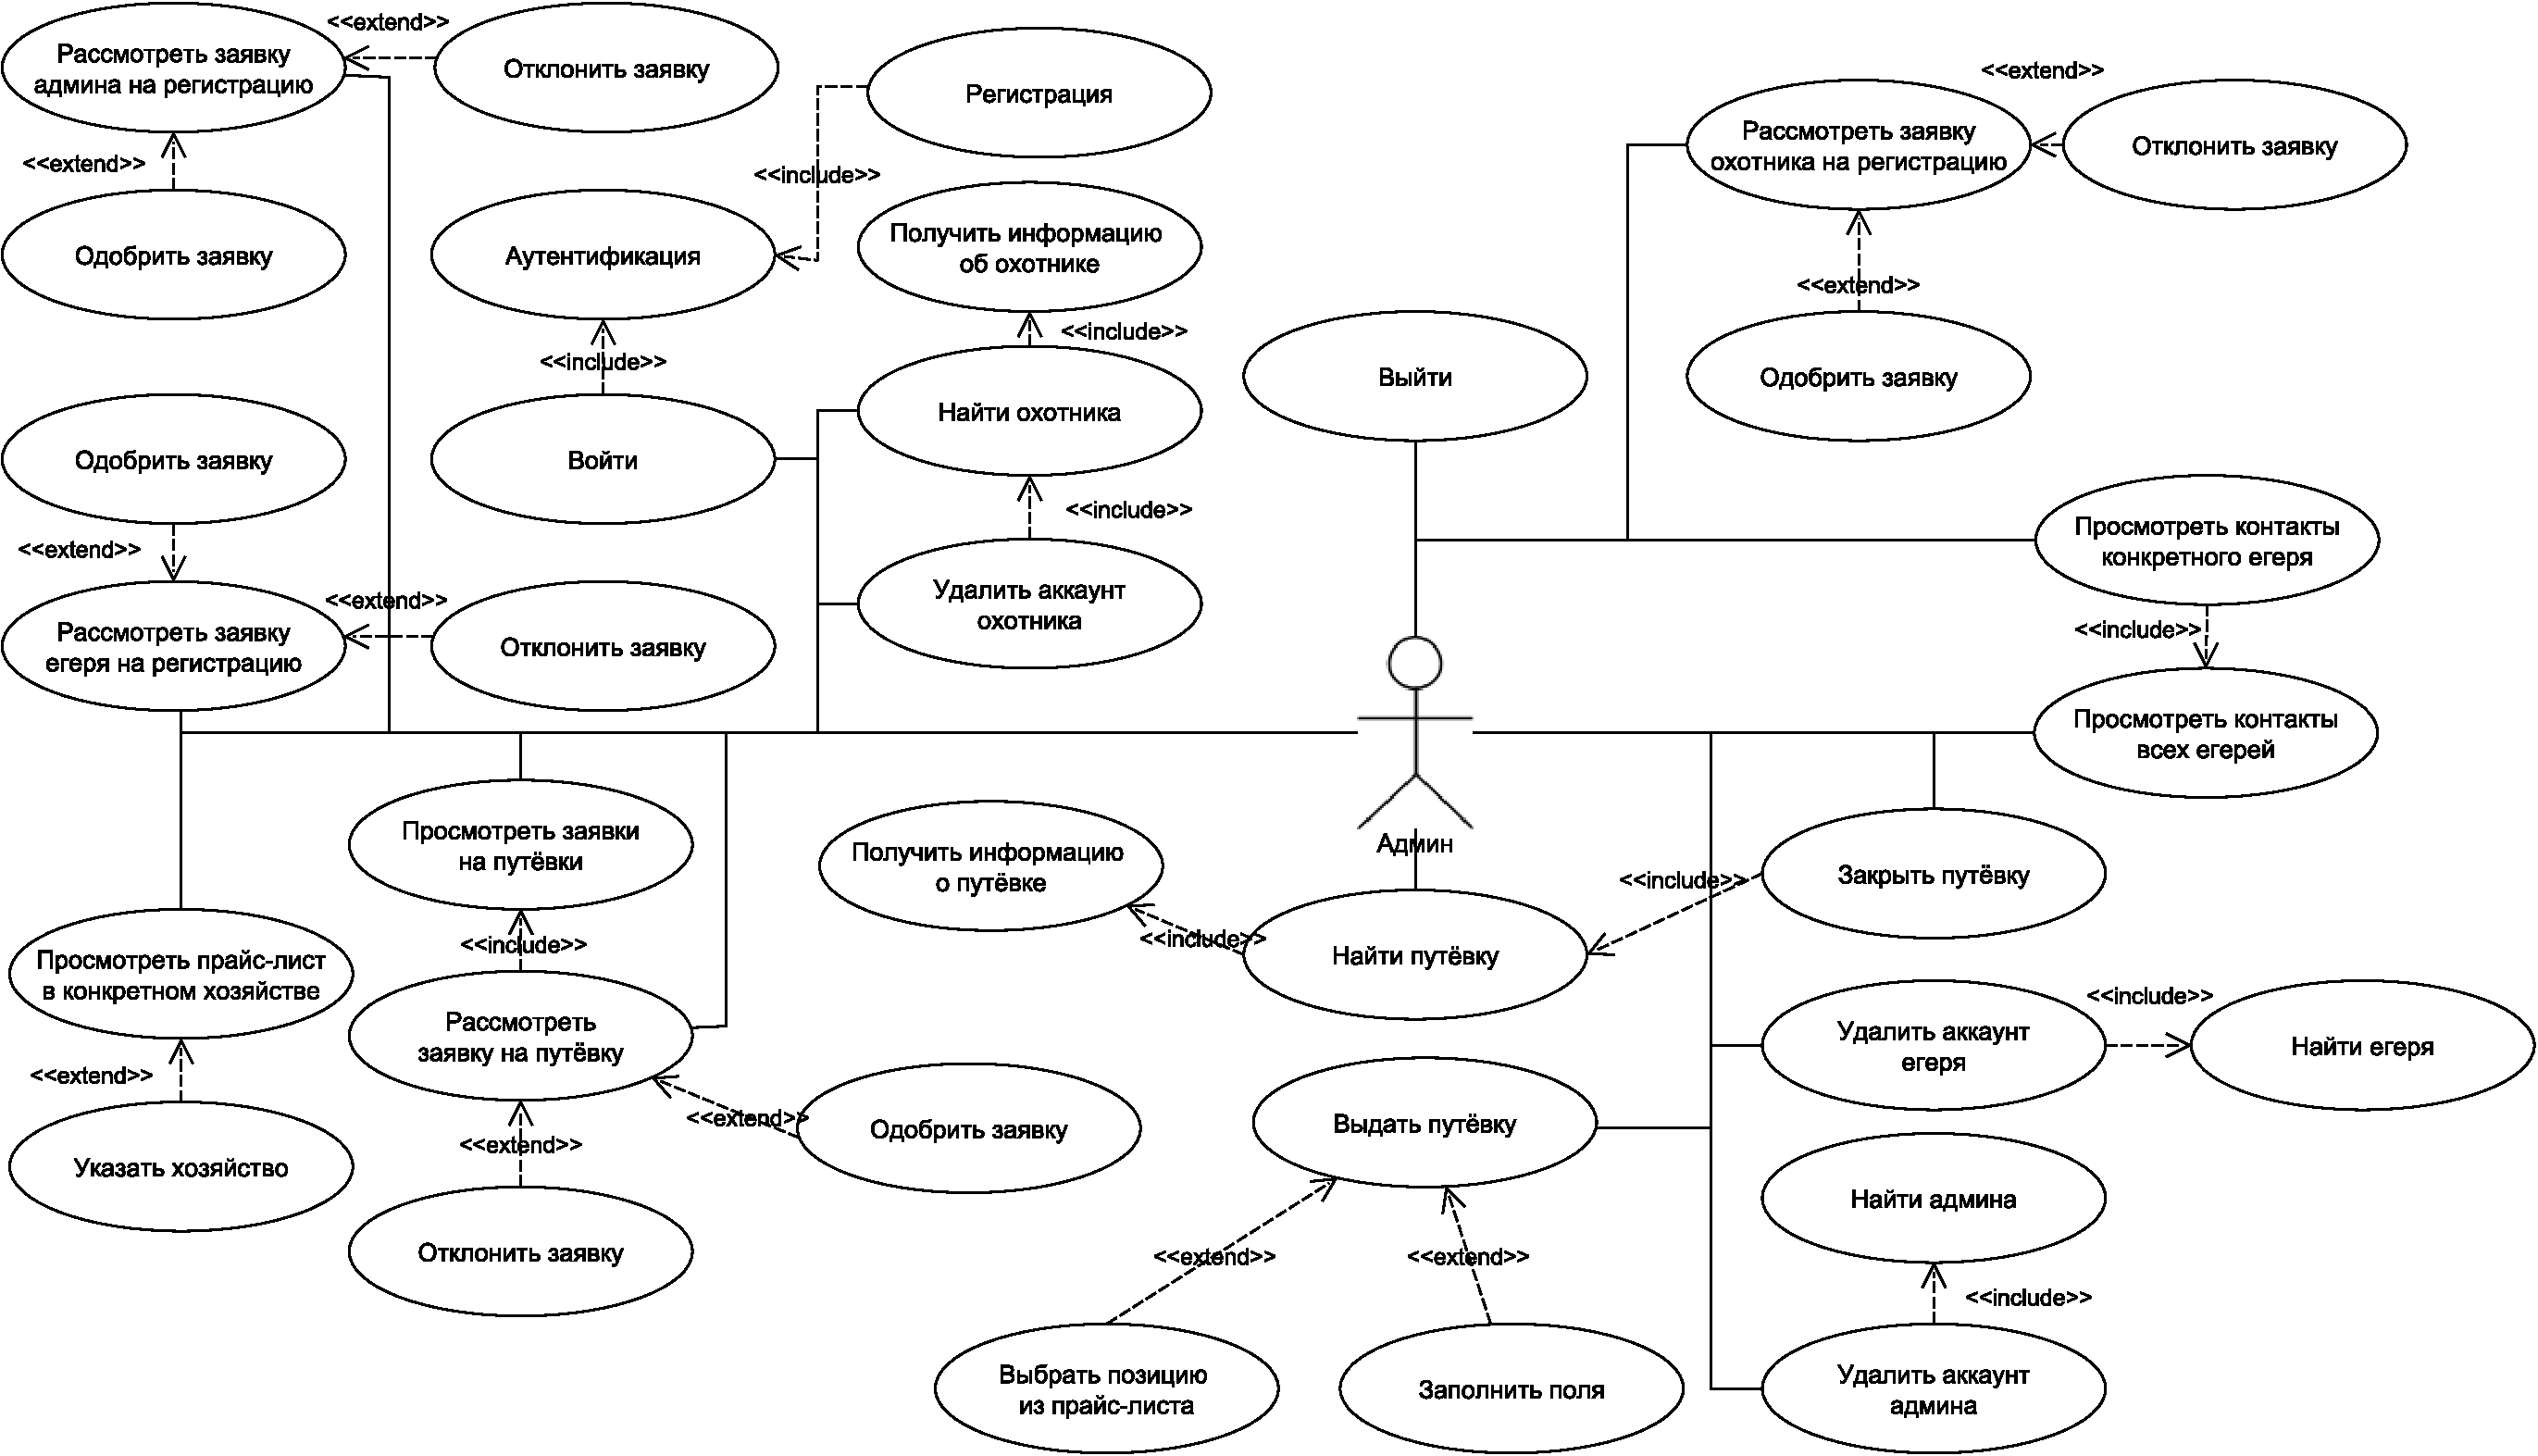
\includegraphics[scale=0.44, angle=90]{schemes/use-case_admin.pdf}}
			\caption{ER-диаграмма сущностей (администратор)}
			\label{fig2:image}
		\end{center}
	\end{figure}

	\begin{figure}[ph!]
		\centering
		\begin{center}
			{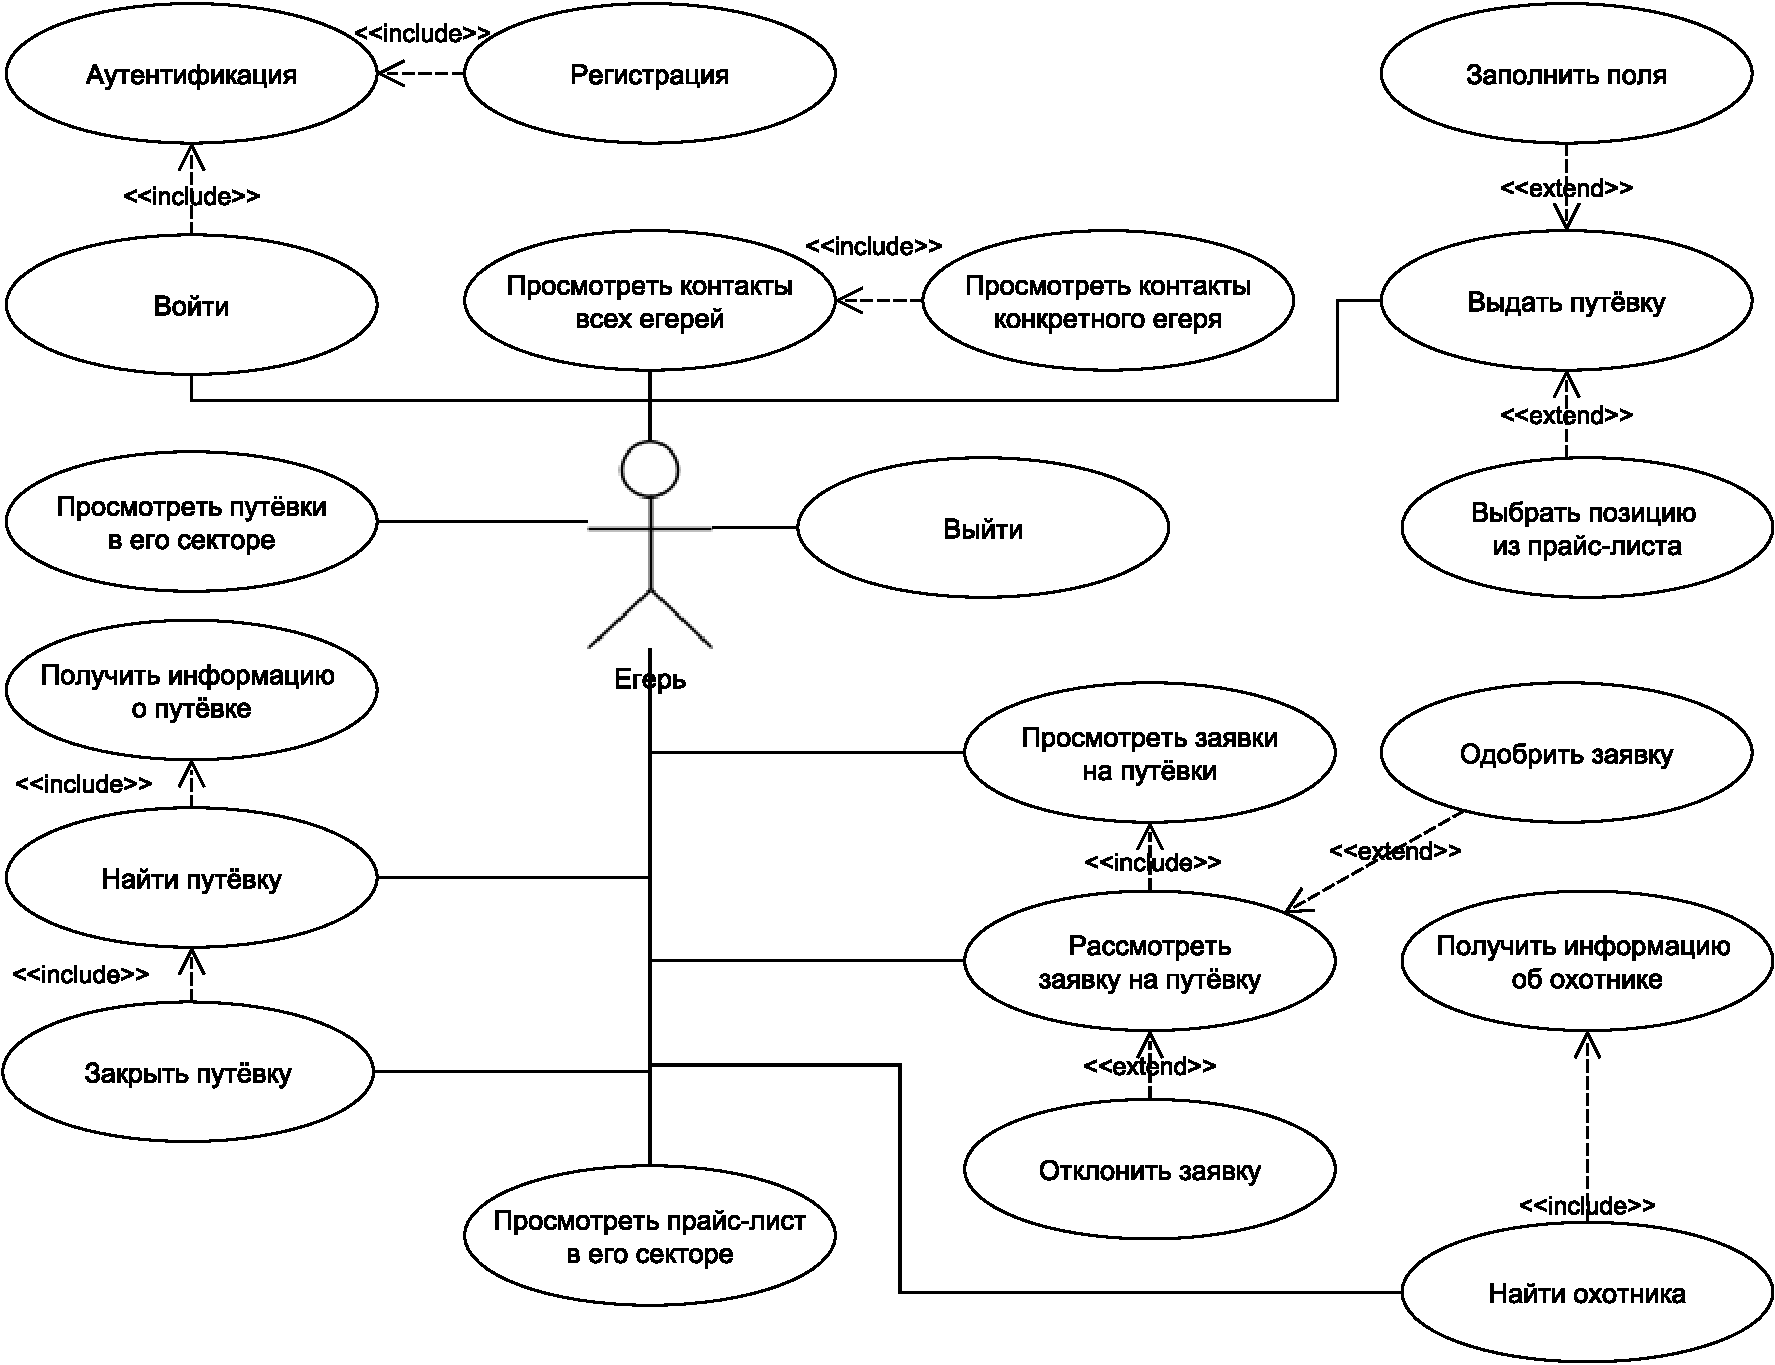
\includegraphics[scale=0.45]{schemes/use-case_huntsman.pdf}}
			\caption{ER-диаграмма сущностей (егерь)}
			\label{fig3:image}
		\end{center}
	\end{figure}

	\begin{figure}[ph!]
		\centering
		\begin{center}
			{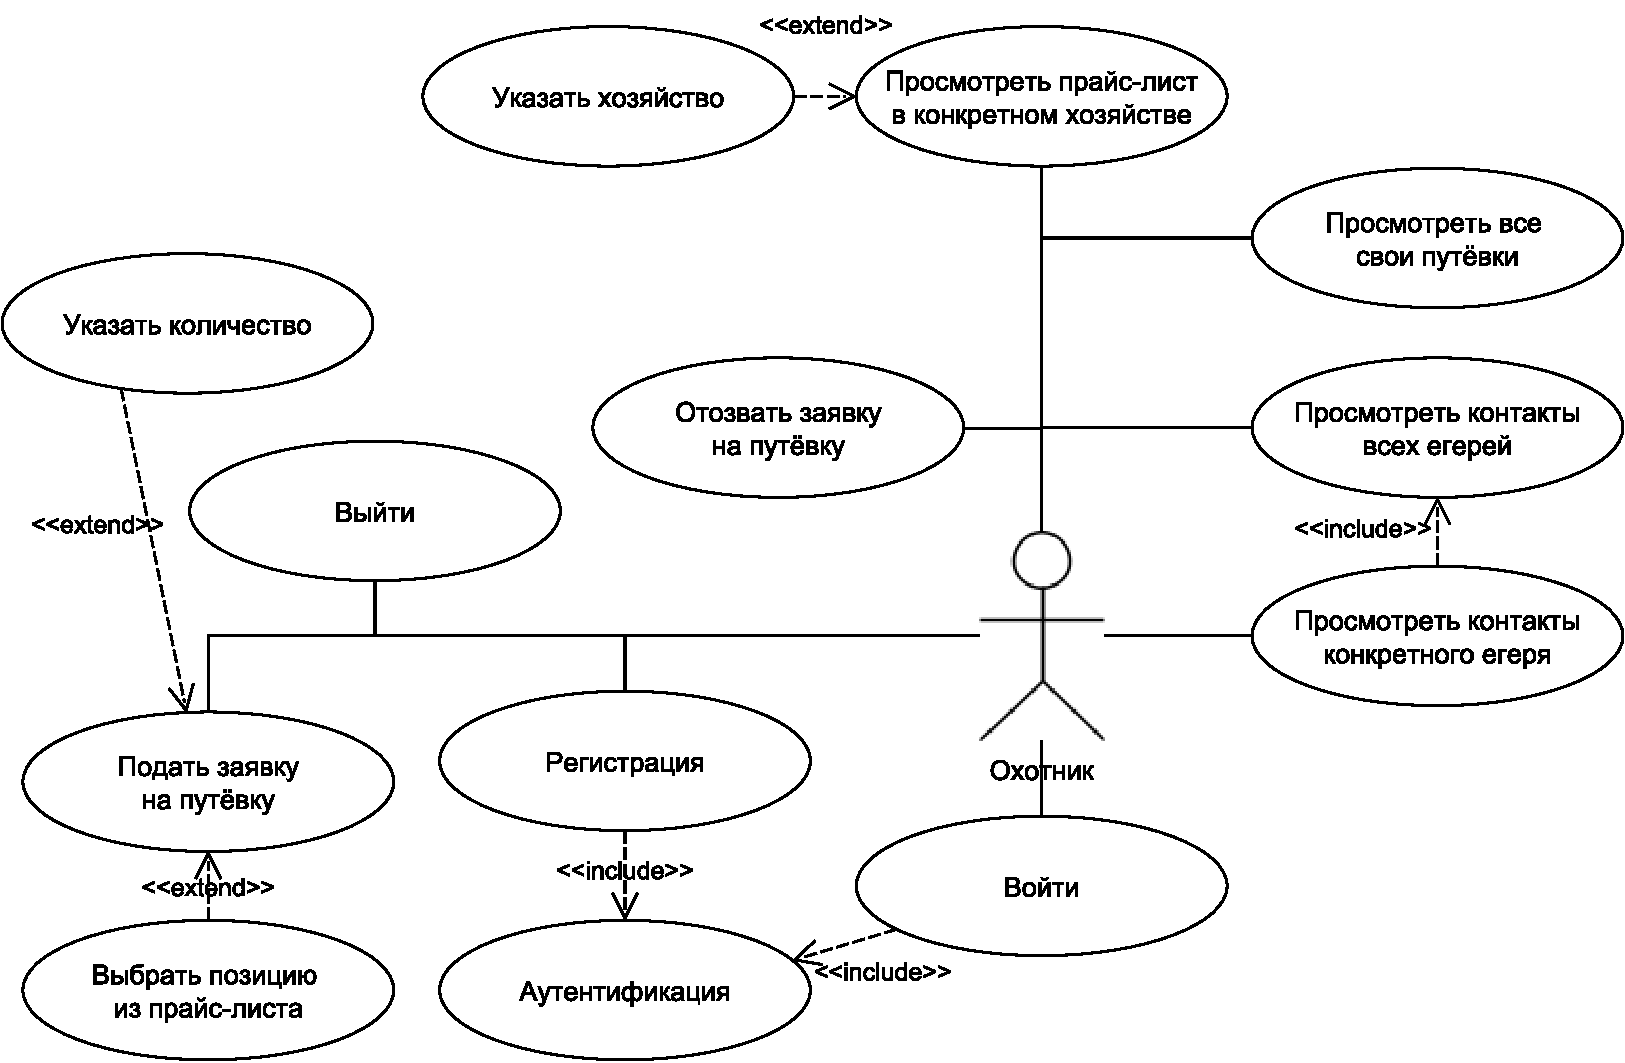
\includegraphics[scale=0.45]{schemes/use-case_hunter.pdf}}
			\caption{ER-диаграмма сущностей (охотник)}
			\label{fig4:image}
		\end{center}
	\end{figure}
	
	\newpage
	
	\subsection{ER-диаграмма сущностей БД}
	На рисунке \ref{fig5:image} приведена ER-диаграмма базы данных, на которой также указываются связи, поля таблиц и ключи.
	
	\begin{figure}[ph!]
		\centering
		\begin{center}
			{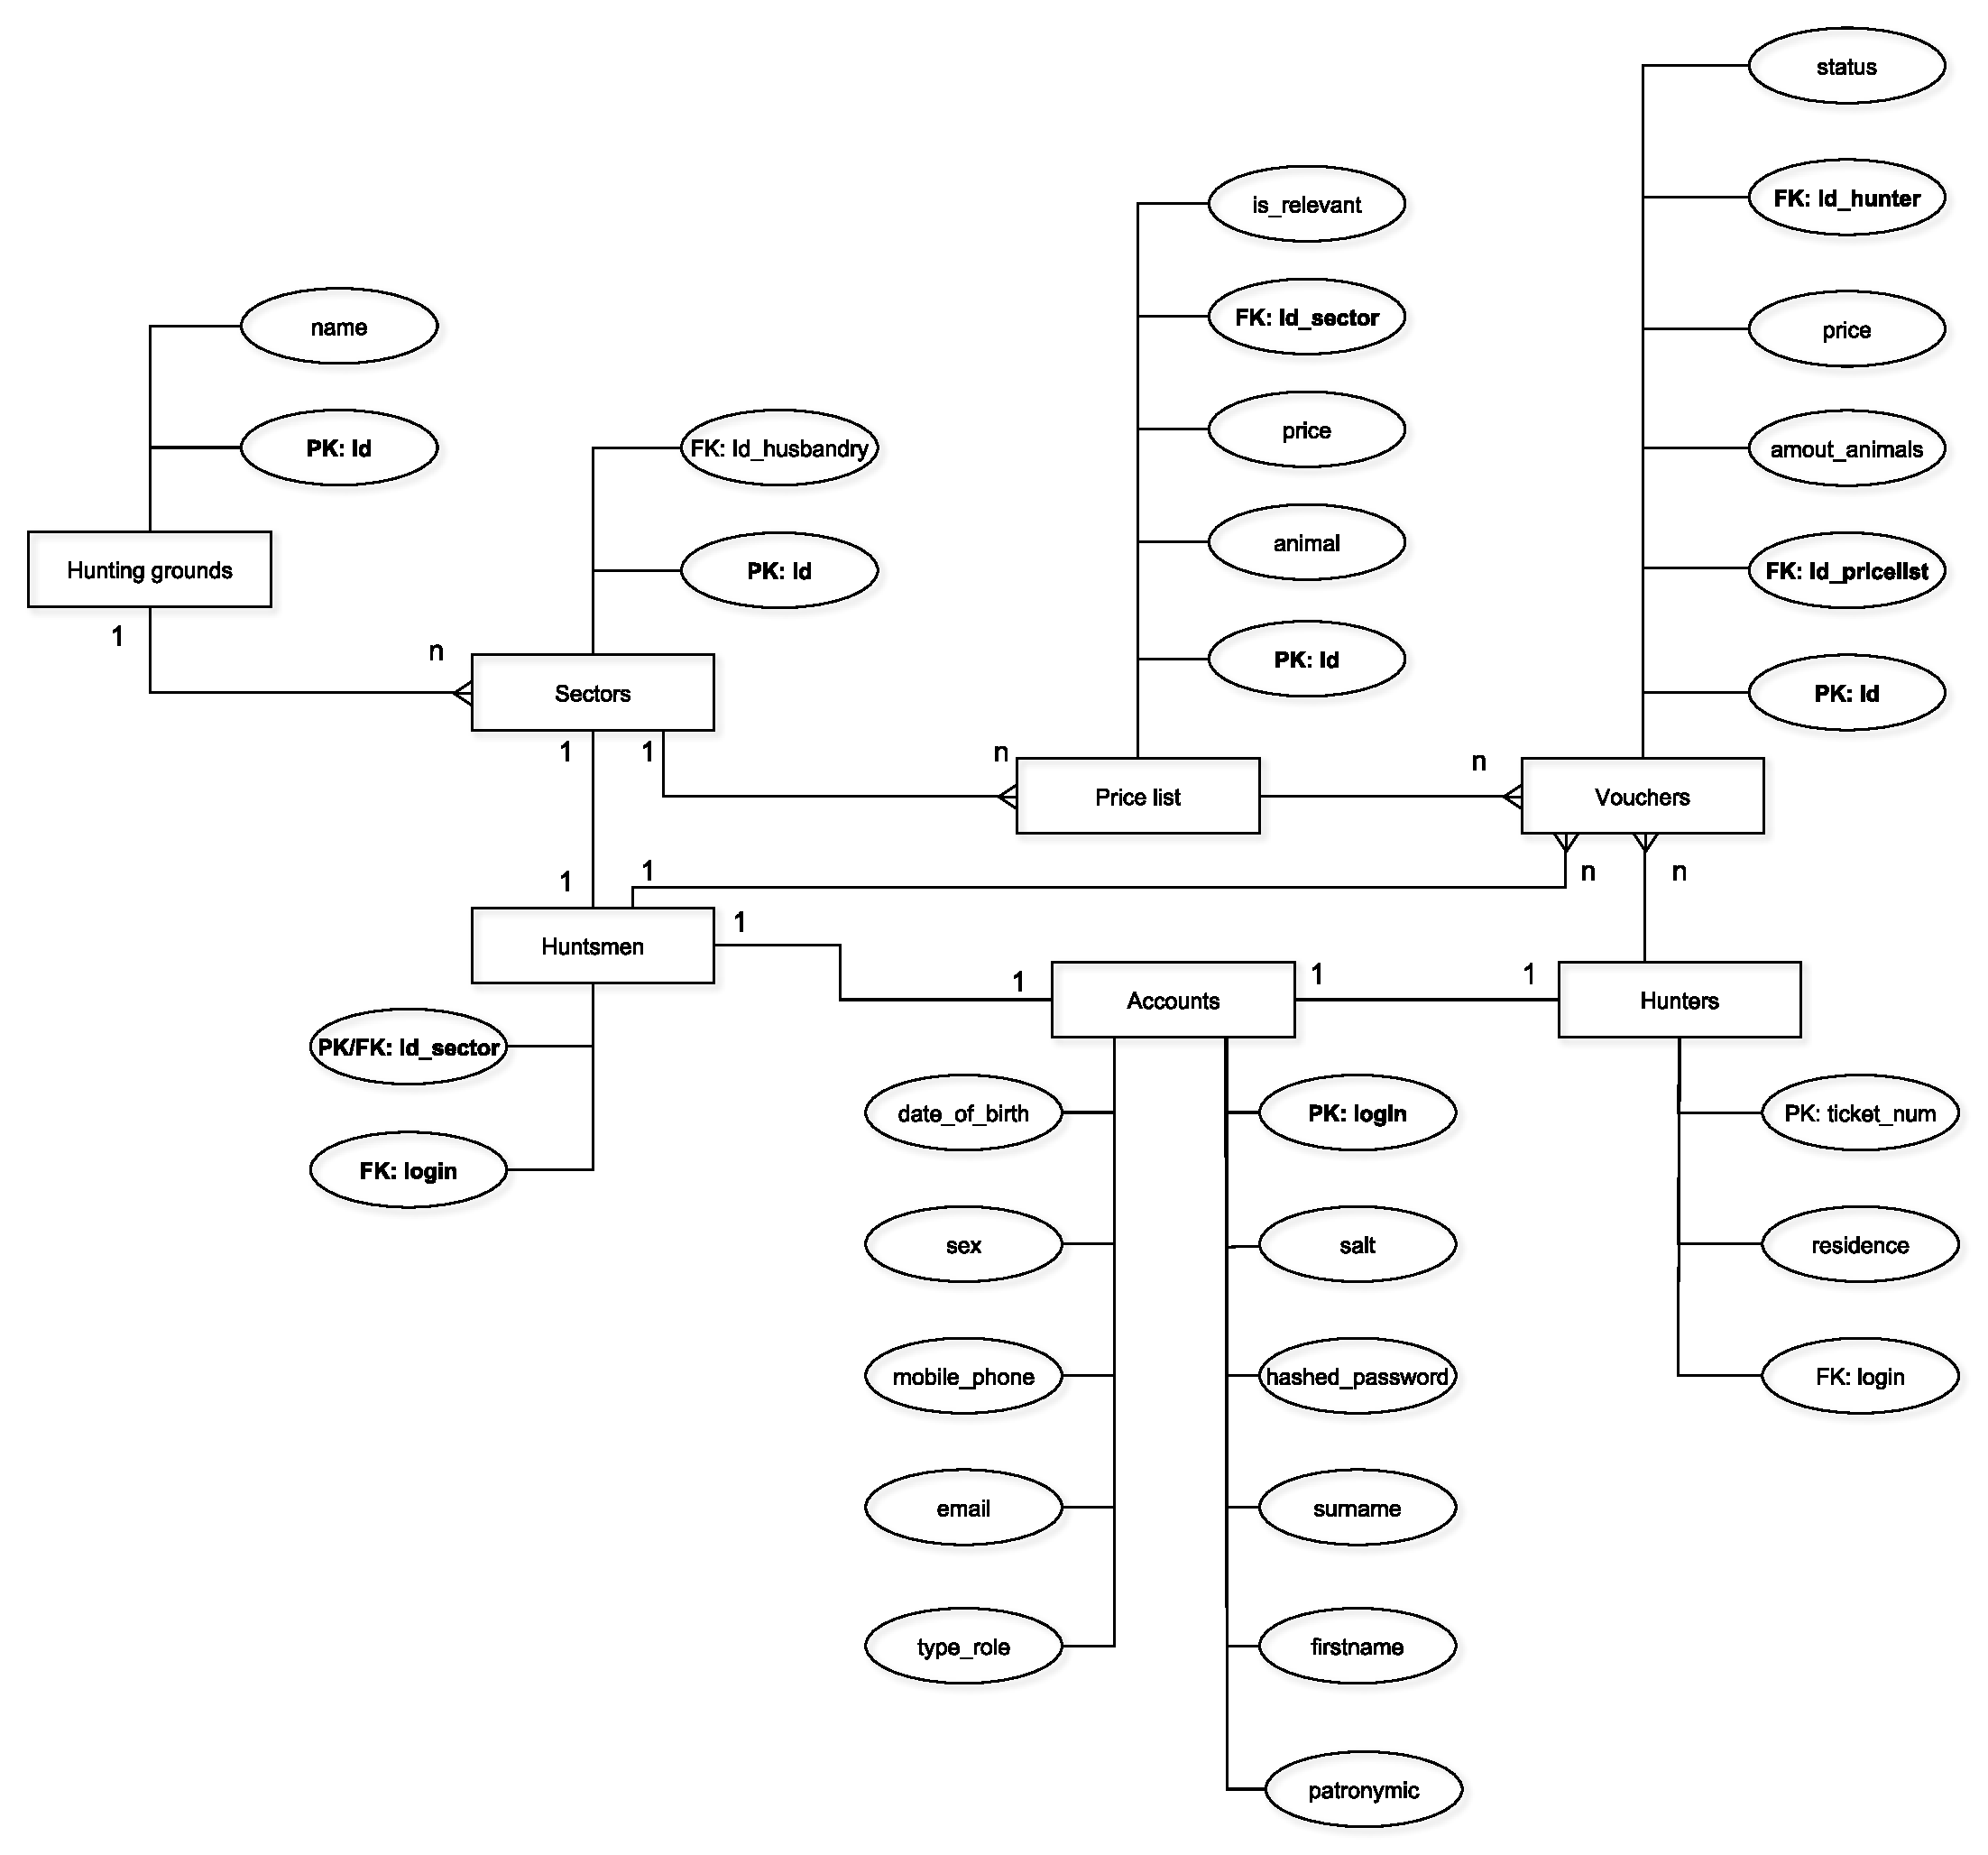
\includegraphics[scale=0.47]{schemes/ERclassic.pdf}}
			\caption{ER-диаграмма сущностей}
			\label{fig5:image}
		\end{center}
	\end{figure}

	\subsubsection{Проектирование базы данных}

	База данных должна содержать таблицы, поля и назначение которых описаны в таблицах 
	\ref{hgtable}-\ref{vouchers_table}.
	
	\begin{table}[h] 
		\begin{center}
			\caption{HuntingGrounds (таблица хозяйств)}
			\label{hgtable}
			\begin{tabular}{| p{3cm} | p{3cm} | p{8cm} |}
				\hline
				\textbf{Атрибут} 	& \textbf{Тип} & \textbf{Значение} \\
				\hline
				Id 					& Целое число &	Идентификатор, PK \\ 
				\hline
				GroundName 			& Строка &	Название \\ 
				\hline
			\end{tabular}
		\end{center}
	\end{table}

	\begin{table}[h] 
		\begin{center}
			\caption{Sectors (таблица секторов)}
			\label{sec_table}
			\begin{tabular}{| p{3cm} | p{3cm} | p{8cm} |}
				\hline
				\textbf{Атрибут} 	& \textbf{Тип} & \textbf{Значение} \\
				\hline
				Id 					& Целое число &	Идентификатор, PK \\ 
				\hline
				IdHusbandry 		& Целое число &	Идентификатор хозяйства, в состав которого входит сектор, FK \\
				\hline
			\end{tabular}
		\end{center}
	\end{table}

	\begin{table}[pt!]
		\begin{center}
			\caption{Accounts (таблица аккаунтов)}
			\label{acc_table}
			\begin{tabular}{| p{3cm} | p{3cm} | p{8cm} |}
				\hline
				\textbf{Атрибут} 	& \textbf{Тип} & \textbf{Значение} \\
				\hline
				Login 				& Строка &	Логин, PK \\ 
				\hline
				Salt 				& Строка &	Соль  \\ 
				\hline
				HashedPassword 		& Строка &	Хэшированный пароль \\ 
				\hline
				Surname 			& Строка &	Фамилия \\ 
				\hline
				Firstname 			& Строка &	Имя \\ 
				\hline
				Patronymic 			& Строка &	Отчество \\ 
				\hline
				DateOfBirth 		& Дата &	Дата рождения \\ 
				\hline
				Sex 				& Символ &	Пол \\ 
				\hline
				MobilePhone 		& Строка &	Мобильный телефон \\ 
				\hline
				Email 				& Строка &	Электронная почта \\ 
				\hline
				TypeRole 			& Строка &	Роль \\ 
				\hline
			\end{tabular}
		\end{center}
	\end{table}

	Для обеспечение безопасности используются хэширование паролей, и в базе данных в таблице \ref{acc_table} хранится только соль и хэшированный пароль.\\

	\begin{table}[pt!] 
		\begin{center}
			\caption{Huntsmen (таблица егерей)}
			\label{huntsmen_table}
			\begin{tabular}{| p{3cm} | p{3cm} | p{8cm} |}
				\hline
				\textbf{Атрибут} 	& \textbf{Тип} & \textbf{Значение} \\
				\hline
				Id 					& Целое число &	Идентификатор сектора, за которым закреплён егерь, PK, FK \\
				\hline
				Login	 			& Строка &	Логин, FK \\ 
				\hline
			\end{tabular}
		\end{center}
	\end{table}

	\begin{table}[pt!] 
		\begin{center}
			\caption{Hunters (таблица охотников)}
			\label{hunters_table}
			\begin{tabular}{| p{3cm} | p{3cm} | p{8cm} |}
				\hline
				\textbf{Атрибут} 	& \textbf{Тип} & \textbf{Значение} \\
				\hline
				TicketNum 			& Строка &	Номер охотничьего билета, PK\\
				\hline
				Residence			& Строка & 	Адрес прописки \\
				\hline
				Login	 			& Строка &	Логин, FK \\ 
				\hline
			\end{tabular}
		\end{center}
	\end{table}

	\begin{table}[pt!]
		\begin{center}
			\caption{PriceList (таблица цен на путёвки)}
			\label{price_table}
			\begin{tabular}{| p{3cm} | p{3cm} | p{8cm} |}
				\hline
				\textbf{Атрибут} 	& \textbf{Тип} & \textbf{Значение} \\
				\hline
				Id 					& Целое число &	Идентификатор, PK\\
				\hline
				Animal				& Строка & 	Название животного \\
				\hline
				Price	 			& Вещественное число &	Цена \\ 
				\hline
				IsRelevant	 		& Логический &	Флаг актуальности \\ 
				\hline
				IdSector	 		& Целое число &	Идентификатор сектора, за которым закреплена позиция, FK \\
				\hline
			\end{tabular}
		\end{center}
	\end{table}

	\begin{table}[pt!] 
		\begin{center}
			\caption{Vouchers (таблица путёвок)}
			\label{vouchers_table}
			\begin{tabular}{| p{3cm} | p{3cm} | p{8cm} |}
				\hline
				\textbf{Атрибут} 	& \textbf{Тип} & \textbf{Значение} \\
				\hline
				Id 					& Целое число &	Идентификатор, PK\\
				\hline
				AmountAnimals		& Целое число & 	Количество животных \\
				\hline
				Price	 			& Вещественное число &	Цена \\ 
				\hline
				IdHunter	 		& Строка &	Идентификатор владельца-охотника, FK \\ 
				\hline
				IdPricelist	 		& Целое число &	Идентификатор позиции из перечня цен, FK \\
				\hline
				Status				& Логический & 	Статус (ждёт решения/одобрено) \\
				\hline
			\end{tabular}
		\end{center}
	\end{table}

	\subsection{Нормальная форма модели}
	1 нф потому
	2/3
	!!!!!!!!!!!!!!!!!!!!!!!!!!!!!!!!!!!!!!!!!!!!!!!!!!!!!!!!!!!!!!!!!!!!!!!!!!!!!!!!!!!!!!!!!!!!!
	
	\subsection{Схемы триггеров}
	!!!!!!!!!!!!!!!!!!!!!!!!!!!!!!!!!!!!!!!!!!!!!!!!!!!!!!!!!!!!!!!!!!!!!!!!!!!!!!!!!!!!!!!!!!!!!

	\subsection{Архитектура приложения. Модель MVC}
	Этот шаблон проектирования предполагает разделение на три отдельных компонента: Модель (Model), Представление (View) и Контроллер (Controller). Это позволяет производить модификации какого-либо компонента независимо от других. \cite{mvc} 
	
	\textbf{Model} - компонент бизнес-логики приложения, предоставляет данные и методы работы с ними.
	
	\textbf{View} - компонент, который отвечает за взаимодействие с пользователем, необходим для отображения данных, полученных в результате работы модели.
	
	\textbf{Controller} отвечает за обработку действий пользователя, перенаправляет данные от пользователя к модели и наоборот.\\
	
	\subsection*{Вывод}
	В разделе были представлены: Use-Case диаграммы для каждой из выделенных ролей (администратора, егеря и охотника), ER-диаграмма сущностей базы данных. Также описана модель MVC, которая была выбрана для дальнейшей реализации.




	
	
	\newpage
	
	\setcounter{table}{0}
	\setcounter{figure}{0}
	\section{Технологическая часть}
	\subsection{Средства реализации программного обеспечения}
		\subsubsection{Язык программирования}
			При разработке программного продукта был использован язык программирования Python (версия 3.7.2) \cite{python}.
			
			Данный выбор был сделан по следующим причинам.
			\begin{enumerate}
				\item[1)] Опыт работы с рассматриваемым языком.
				\item[2)] Поддержка ООП.
				\item[3)] Большое количество литературы, связанной с ЯП Python.
			\end{enumerate}
		
			В качестве среды разработки были использованы PyCharm \cite{pycharm} и Visual Studio Code \cite{vcode}, поскольку они бесплатны для студентов, удобны в процессе разработки и ранее активно использовались.

		\subsubsection{СУБД}
		Одними из наиболее популярных СУБД, используемых в настоящее время, являются Oracle, MySQL, Microsotf SQL сервер и PostgreSQL. В таблице \ref{cmptable} приведено их сравнение.
		
		\begin{table}[pt!] 
			\begin{center}
				\caption{Сравнение СУБД}
				\label{cmptable}
				\begin{tabular}{| p{4cm} | p{5cm} | p{5cm} |}
					\hline
					\textbf{СУБД} 	& \textbf{Преимущества} & \textbf{Недостатки} \\
					\hline
					Oracle 			& - Широкий функционал & - Платное использование \\ 
									& - Ориентирован на работу с большими БД & - Необходимость в дополнительных ресурсах \\
					\hline
					MySQL 			& - Есть бесплатная версия & - Есть платные версии для коммерческого использования\\
									& - Исчерпывающая документация & - Для бесплатной версии доступна только платная поддержка \\ 
									& - Простой интерфейс & - Отсутствует встроенная поддержка XML \\
									& - Хорошо справляется с большими объёмами данных &  \\
					\hline
					Microsotf SQL сервер  	& - Низкий порог вхождения &- Высокая цена для юридических лиц \\
					 				& - Стабильность в работе & - Требуется много дополнительных ресурсов \\ 
									& - Возможность регулировать и отслеживать уровень производительности &  \\
					\hline
					PostgreSQL 		& - Бесплатная & - Низкая скорость выполнения пакетных операций \\ 
									& - Подробная документация & - Поддерживается не всеми библиотеками \\
									& - Поддержка json &  \\
					\hline
				\end{tabular}
			\end{center}
		\end{table}
	\newpage
	
	При выборе СУБД особо выделялось такое преимущество, как доступность приложения. Немаловажную роль играет и хорошая, полная документация. Перечисленными преимуществами обладает такая СУБД, как PostgreSQL. Это средство было выбрано для реализации текущей задачи, так как дополнительно есть опыт работы с ней.
	
	Что касается ORM (Object-relational mapping), то был выбран peewee \cite{peewee}, поскольку он поддерживает PostgreSQL и является распространённые решением для выбранного языка.
	
	\subsubsection{Web-фреймворк}
	Django \cite{django} был выбран в качестве Web-фреймворка по следующим причинам.
	\begin{itemize}
		\item Использует шаблон проектирования MVC, который был выбран ранее.
		\item Работает с большим количеством дополнительных функций, которые значительно упрощают работу с аутентификацией пользователя, картами сайта и т.д.
		\item Масштабируемость. За счёт архитектуры данного фреймворка его компоненты являются достаточно независимыми, что позволяет легче расширять его функционал.
	\end{itemize}

	\subsection{UML-диаграммы}
		\subsubsection{Компонент доступа к данным}
		Доступ к данным реализован с помощью паттерна проектирования Repository. Соответствующая UML-диаграмма представлена на рисунке \ref{fig6:image}.
		
		\begin{figure}[ph!]
			\centering
			\begin{center}
				{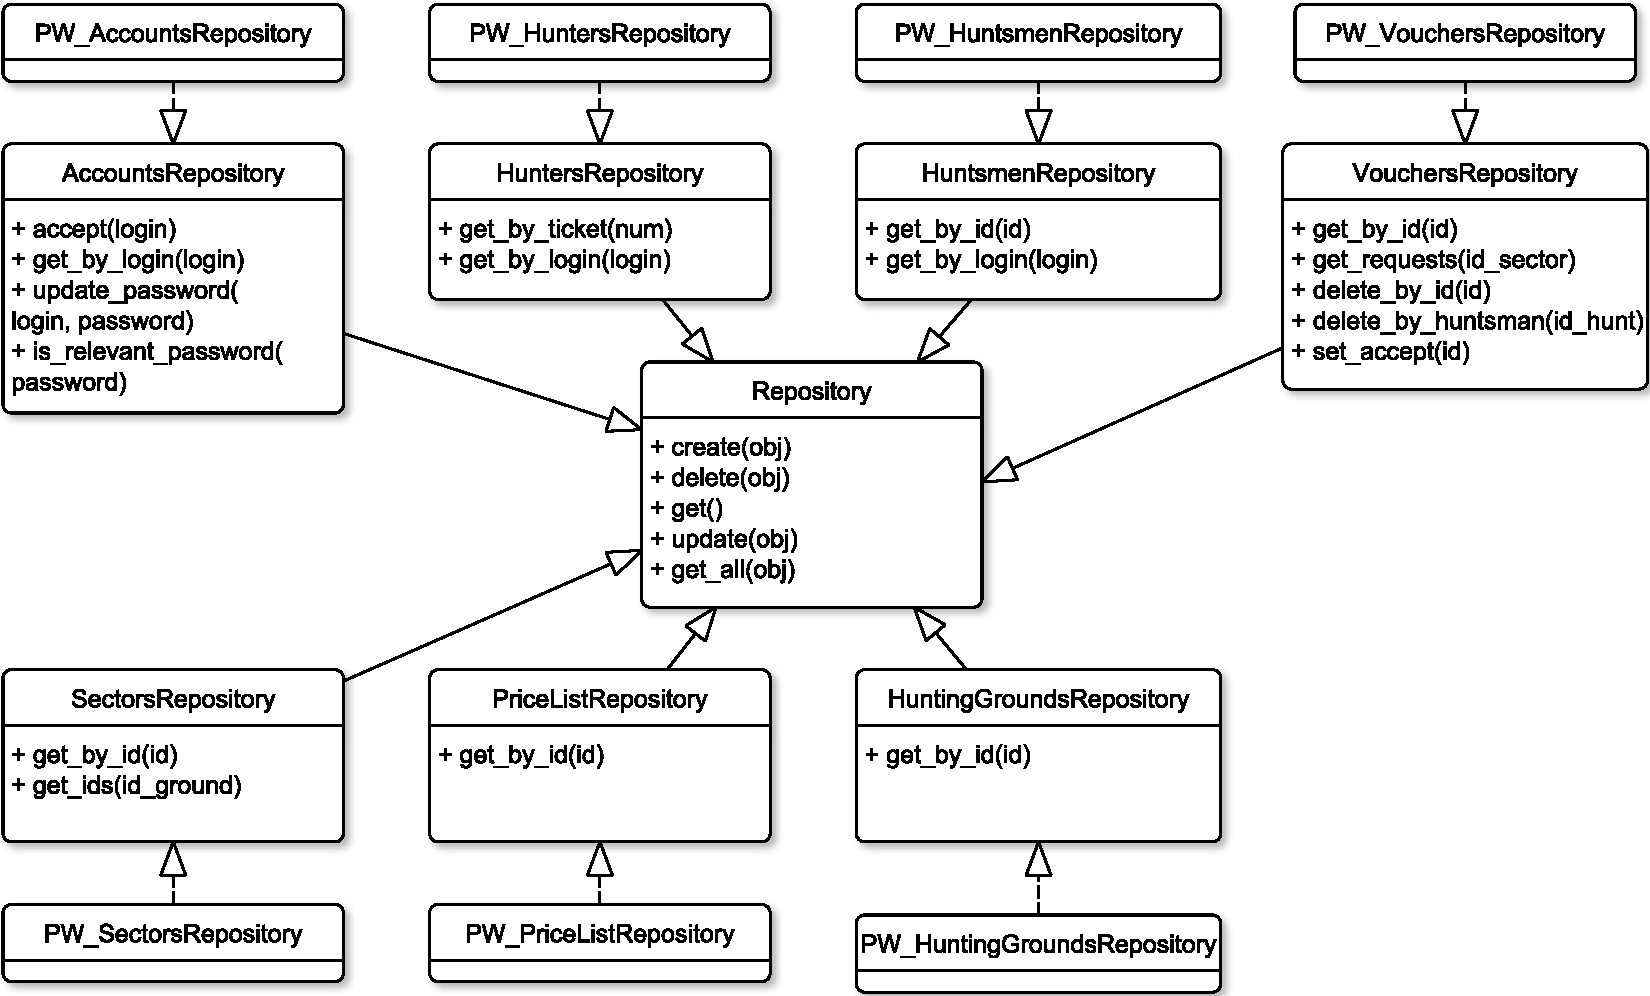
\includegraphics[scale=0.6]{schemes/uml_access_rep.pdf}}
				\caption{UML-диаграмма компонента доступа к данным}
				\label{fig6:image}
			\end{center}
		\end{figure}
		\newpage
	
		\subsubsection{Компонент бизнес-логики}
		Этот компонент выполняет основную обработку данных, соответствующая UML-диаграмма представлена на рисунке \ref{fig7:image}.
		
		\begin{figure}[ph!]
			\centering
			\begin{center}
				{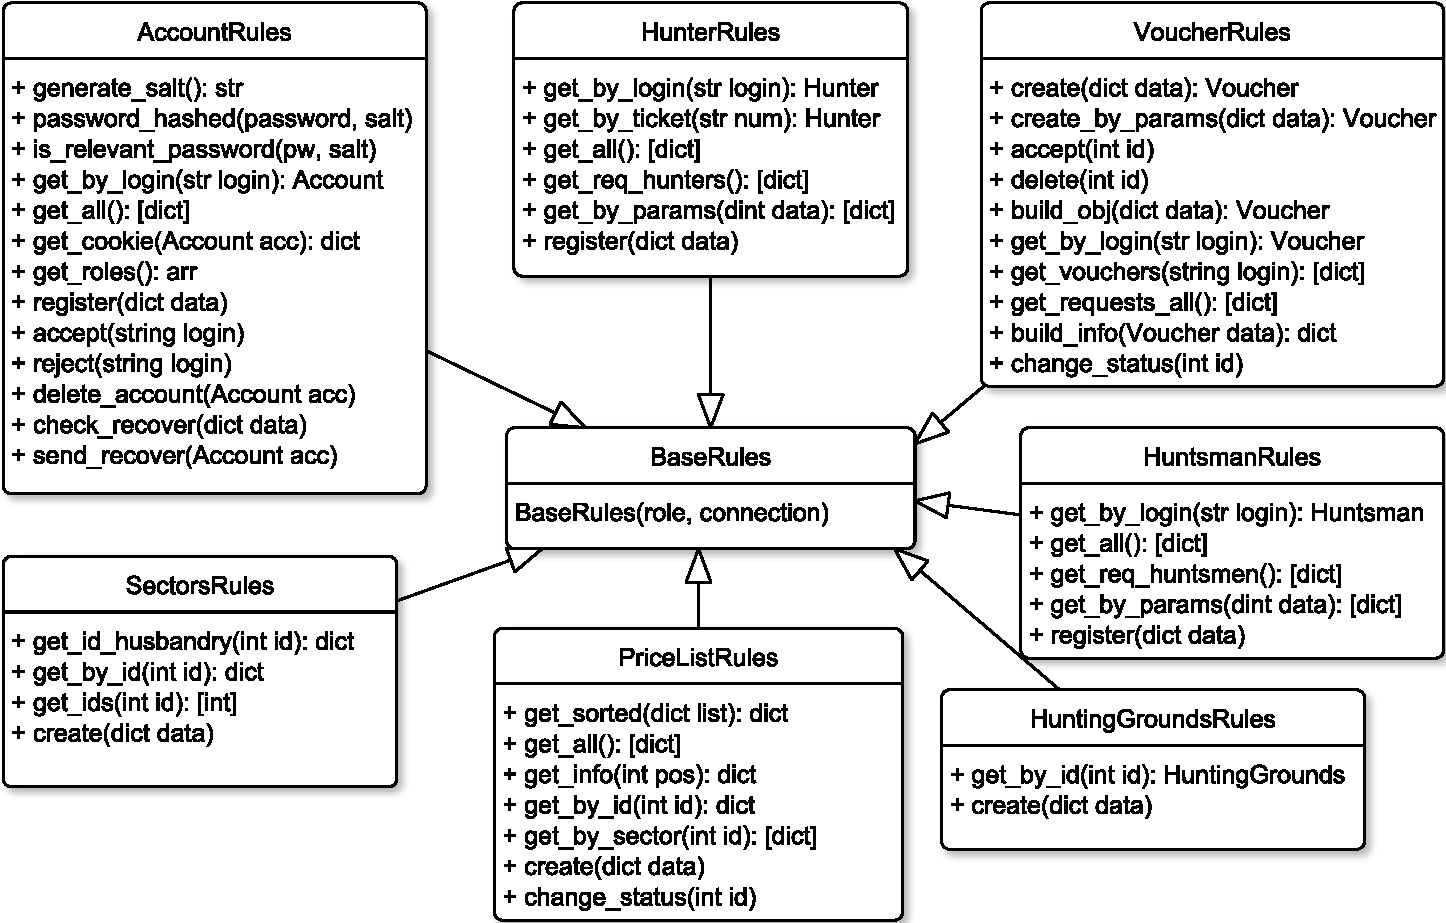
\includegraphics[scale=0.6]{schemes/uml_business.pdf}}
				\caption{UML-диаграмма компонента бизнес-логики}
				\label{fig7:image}
			\end{center}
		\end{figure}
	
		\subsubsection{Компонент представления}
		UML-диаграмма компонента, отвечающего за отображение web-страниц, изображена на рисунке \ref{fig8:image}.
		
		\begin{figure}[pt!]
			\centering
			\begin{center}
				{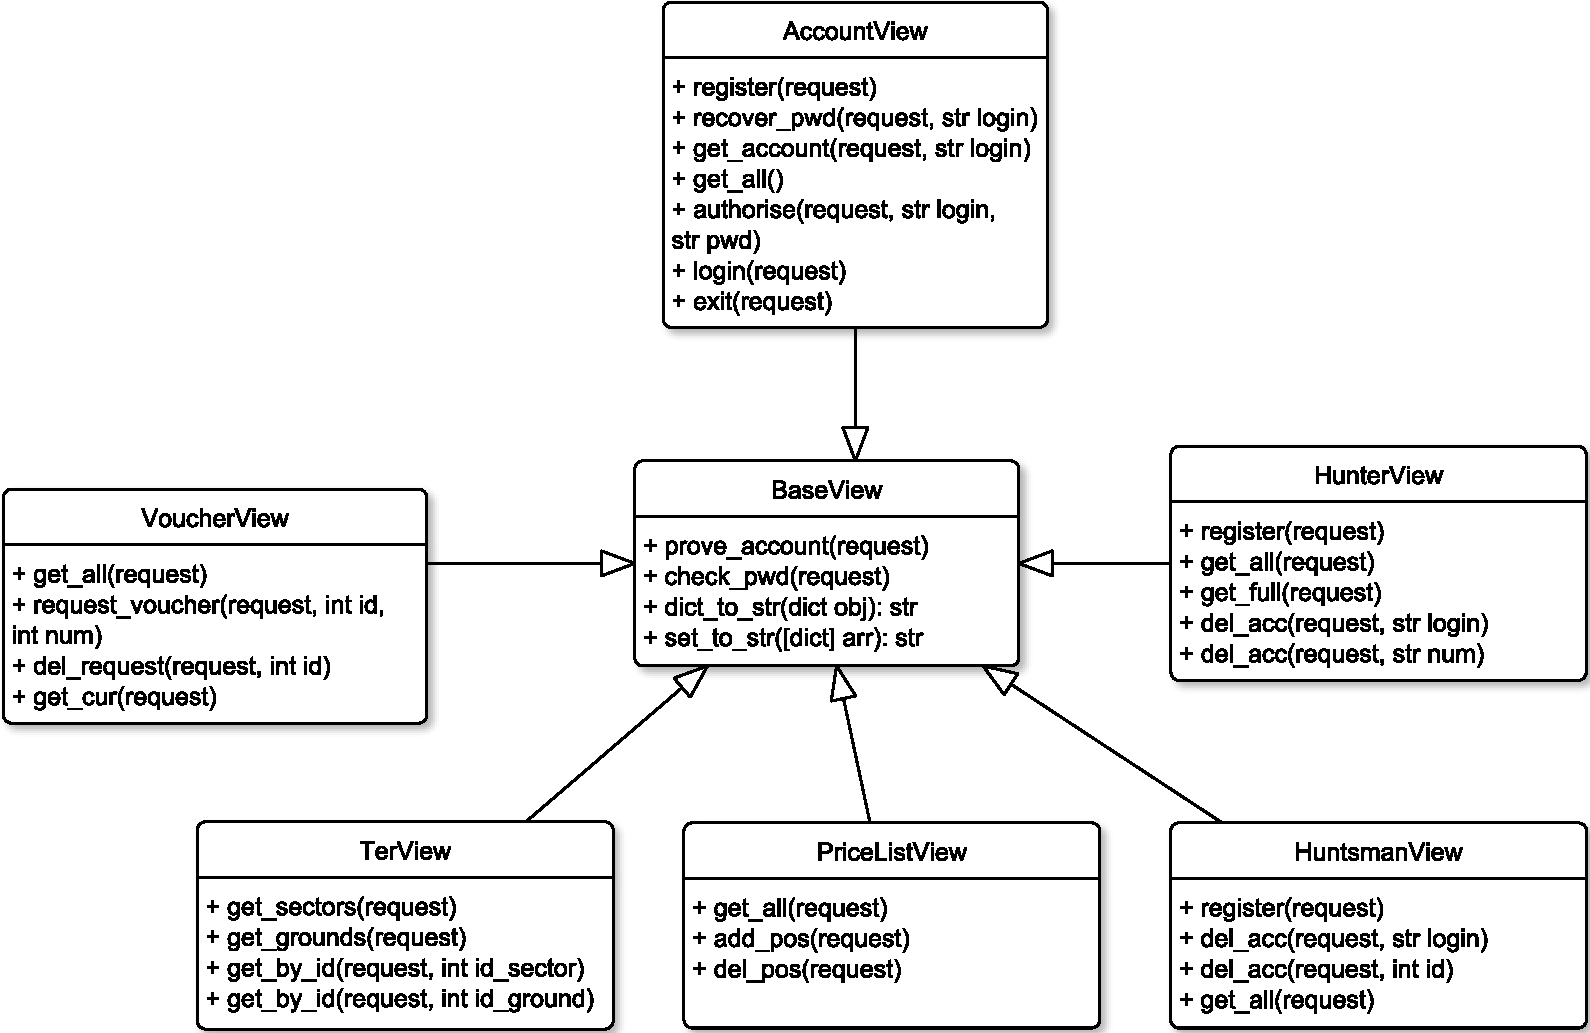
\includegraphics[scale=0.6]{schemes/webGUI.pdf}}
				\caption{UML-диаграмма компонента представления}
				\label{fig8:image}
			\end{center}
		\end{figure}
		\newpage
	
		\subsubsection{Диаграмма приложения}
		Все приведённые выше UML-диаграммы \ref{fig6:image}-\ref{fig8:image} можно объединить в одну - диаграмму-приложения, которая находится на рисунке \ref{fig9:image}.
		
		\begin{figure}[ph!]
			\centering
			\begin{center}
				{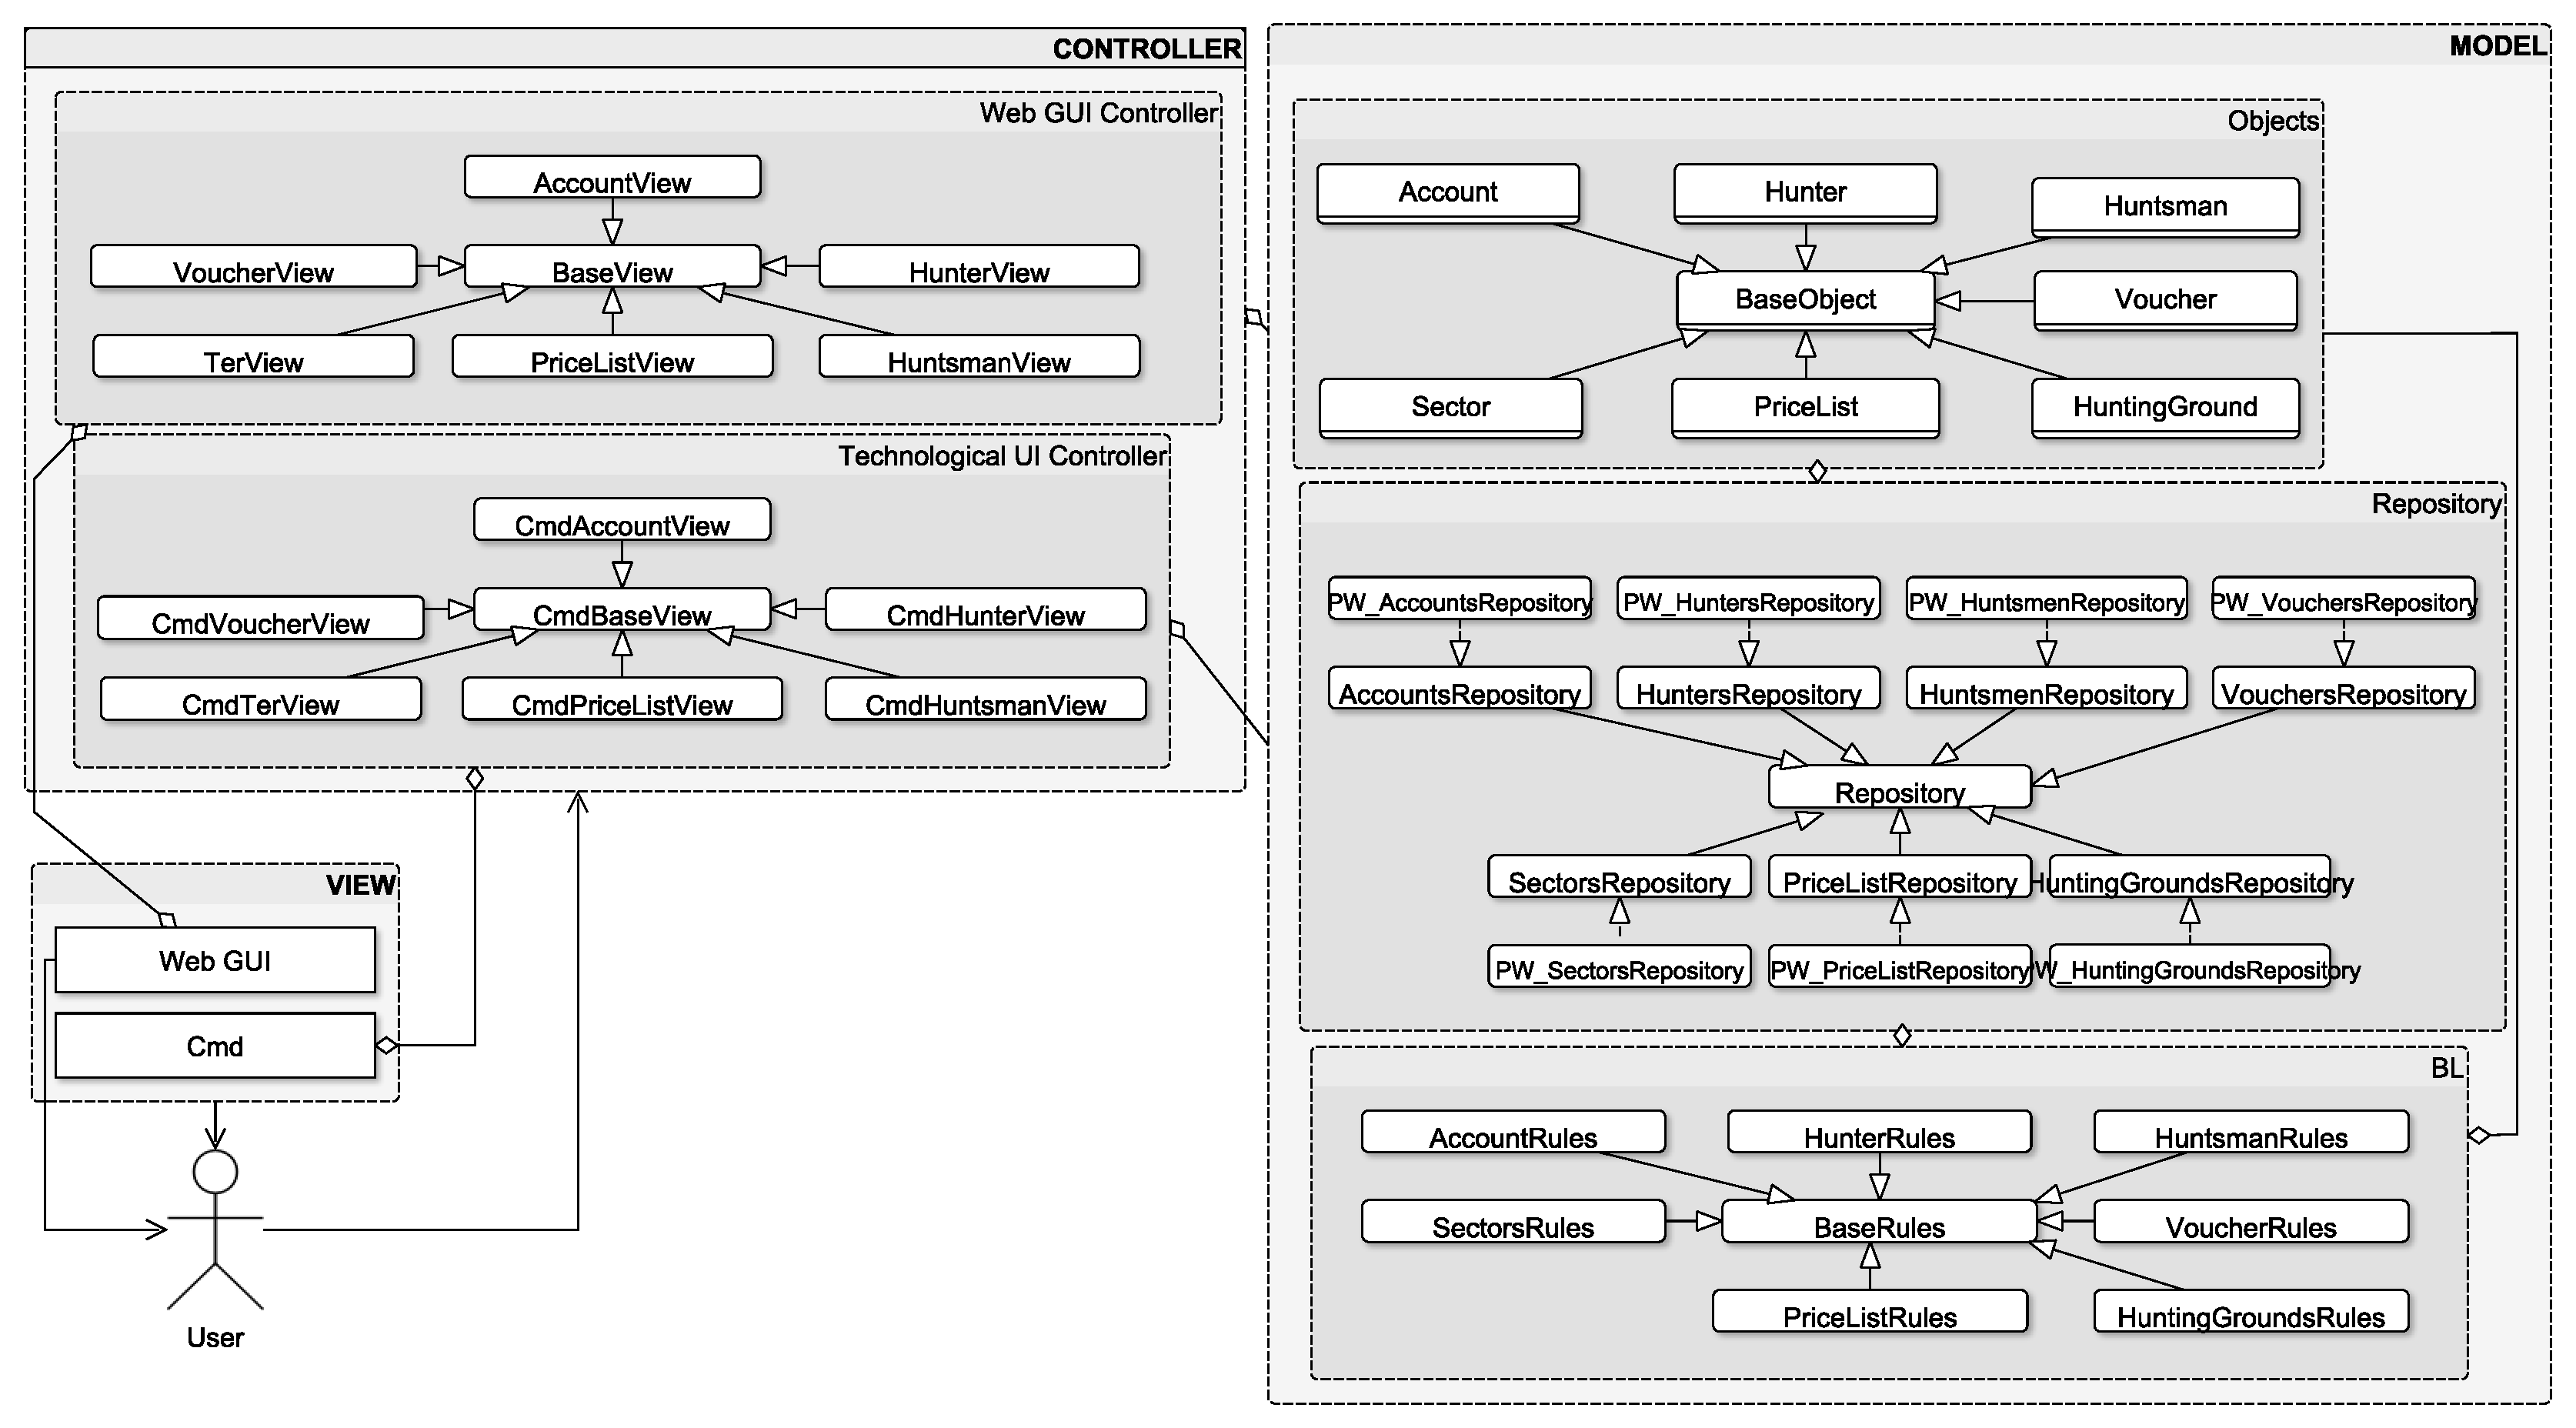
\includegraphics[scale=0.44, angle=90]{schemes/uml_full.pdf}}
				\caption{UML-диаграмма компонента бизнес-логики}
				\label{fig9:image}
			\end{center}
		\end{figure}
	\newpage
	
	\subsection{Реализация базы данных}	
		\subsubsection{Создание таблиц}
		В соответствии с моделью были созданы 7 таблиц. Создание некоторых из них, а именно accounts, hunters, huntsmen представлено в листинге \ref{lst:create_tables}.
		
		\begin{lstlisting}[caption = {Создание некоторых таблиц}, label=lst:create_tables]
CREATE TABLE IF NOT EXISTS accounts(
	login VARCHAR(20) PRIMARY KEY,
	salt TEXT,
	hashed_password TEXT,
	surname VARCHAR(30) NOT NULL,
	firstname VARCHAR(30) NOT NULL,
	patronymic VARCHAR(30),
	date_of_birth DATE NOT NULL,
	sex CHAR NOT NULL,
	mobile_phone VARCHAR(30) NOT NULL,
	email VARCHAR(50) NOT NULL,
	type_role VARCHAR(10) NOT NULL
);

CREATE TABLE IF NOT EXISTS huntsmen(
	id INTEGER REFERENCES sectors,
	PRIMARY KEY (id),
	login VARCHAR(20) REFERENCES accounts
);

CREATE TABLE IF NOT EXISTS hunters(
	ticket_num TEXT PRIMARY KEY,
	residence VARCHAR(100) NOT NULL,
	login VARCHAR(20) REFERENCES accounts
);
		\end{lstlisting}
	
		В таблице accounts первичный ключ - login (логин пользователя), атрибуты surname, firstname, patronymic, mobile\_phone, email, type\_role имеют органичения в несколько символов, также дата рождения имеет специальный тип - дата. В основном, на все поля выставлено ограничение NOT NULL, поскольку эти поля обязательны и заполняются пользователем (это не касается отчества, поскольку его может не быть). Касаемо двух других таблиц, то у них выставлены такие же ограничения.
		
		В таблице huntsmen первичный ключ - id (идентификатор сектора, за которым он закреплён), он же и внешний ключ, который ссылается на одноимённое поле в таблице sectors, также внешним ключом является атрибут login, указывающий на соответствующее поле в таблице accounts.
		
		ticket\_num (номер охотничьего билета) - первичный ключ в таблице hunters, а login также как и в таблице huntsmen выступает в качестве внешнего ключа на таблицу accounts.
			
		\subsubsection{Наполнение таблиц}
		Таблицы заполняются сгенерированными данными с помощью библиотеки Faker. Полученные данные записываются в файл, из которого далее будут подгружаться данные. На листингах \ref{lst:create_faker1}-\ref{lst:create_faker2} приведены функции генерации данных для таблицы аккаунтов (accounts) и путёвок (vouchers), примеры таких функций. Другие таблицы заполняются аналогично.
		
		\begin{lstlisting}[caption = {Генерация данных для таблицы accounts}, label=lst:create_faker1]
def generate_accounts():
	fake = Faker()
	fake_ru = Faker('ru_Ru')
	
	f = open('accounts.cvg', 'w')
	
	i = 0
	while i < NUM_SECTORS + MAX_AMOUNT:
		sex_p = choice(sex)
		if sex_p == 'м':
			surname = fake_ru.last_name_male()
			name = fake_ru.first_name_male()
			patronymic = fake_ru.middle_name_male()
		else:
			surname = fake_ru.last_name_female()
			name = fake_ru.first_name_female()
			patronymic = fake_ru.middle_name_female()
		
		date_of_brth = fake_ru.date_of_birth(None, 21, 80)
		phone = fake_ru.phone_number()
		email = fake_ru.email()
		
		lgn = surname[:3] + name[:2] + '_' + str(date_of_brth).split('-')[2] + \
		'_' + str(date_of_brth).split('-')[1] + \
		'_' + str(date_of_brth).split('-')[0]
		lgn = pytils.translit.translify(lgn)
		login.append(lgn)
		
		pswd = fake.password(length=8, special_chars=False, digits=True, upper_case=True, lower_case=True)
		salt = uuid.uuid4().hex
		salt_pw = pswd.encode('utf-8') + salt.encode('utf-8')
		hashed_pswd = hashlib.sha256(salt_pw).hexdigest()
		
		if i < NUM_SECTORS:	status = 'егерь'
		else:				status = 'охотник'
		
		line = "{0}|{1}|{2}|{3}|{4}|{5}|{6}|{7}|{8}|{9}|{10}\n".format(
			lgn, salt, hashed_pswd, surname, name,
			patronymic, date_of_brth, sex_p, phone, email, status)
		f.write(line)
		
		i += 1
	
	f.close()
		\end{lstlisting}
	
	\begin{lstlisting}[caption = {Генерация данных для таблицы vouchers}, label=lst:create_faker2]
def generate_vouchers():
	f = open('vouchers.cvg', 'w')
	
	for i in range(MAX_AMOUNT + 200):
		duration = choice(range(1, 100))
		amount = choice(range(1, 10))
		prc = 0
		ind = choice(range(1, MAX_AMOUNT))
		id_hunter = hunters[ind]
		id_pricelist = choice(range(1, MAX_AMOUNT))
		
		line = "{0}|{1}|{2}|{3}|{4}\n".format(duration, amount, prc, id_hunter, id_pricelist)
		
		f.write(line)
	f.close()
	\end{lstlisting}
		
		
		\subsubsection{Реализация триггеров}
		Были реализованы триггеры в соответствии с требованиями, которые описывались ранее. 
		
		На листинге \ref{lst:trigger1} приведён триггер ProhibitDelAdmin, препятствующий удалению аккаунта администратора, в случае, если он остался единственным в системе.
		
		\begin{lstlisting}[caption = {Реализация триггера ProhibitDelAdmin}, label=lst:trigger1]
CREATE OR REPLACE FUNCTION ProhibitDelAdmin()
RETURNS TRIGGER
AS $$
BEGIN	
	IF OLD.type_role = 'админ' AND (
		SELECT count(*)
		FROM accounts
		WHERE type_role = 'админ') < 2
	THEN
		RAISE EXCEPTION 'Profibited to delete a single admin';
	END IF;
	RETURN OLD;
END;
$$
LANGUAGE PLpgSql;

CREATE TRIGGER ProhibitDelAdmin
BEFORE DELETE ON accounts
FOR EACH ROW
EXECUTE PROCEDURE ProhibitDelAdmin();
		\end{lstlisting}
	
		На листинге \ref{lst:trigger2} приведёна реализация триггера FullDelHunter, каскадно удаляющего записи в других таблицах, связанных с удаляемым охотником.
		
		\begin{lstlisting}[caption = {Реализация триггера FullDelHunter}, label=lst:trigger2]
CREATE OR REPLACE FUNCTION FullDelHunter()
RETURNS TRIGGER
AS $$
BEGIN	
	IF OLD.type_role != 'охотник'
	THEN
	RETURN OLD;
	END IF;
	DELETE FROM vouchers
	WHERE vouchers.id_hunter IN (
		SELECT hunters.ticket_num
		FROM hunters
		WHERE hunters.login = OLD.login);
	
	DELETE FROM hunters
	WHERE hunters.login = OLD.login;
	RETURN OLD;
END;
$$
LANGUAGE PLpgSql;

CREATE TRIGGER FullDelHunter
BEFORE DELETE ON accounts
FOR EACH ROW
EXECUTE PROCEDURE FullDelHunter();
		\end{lstlisting}
	
	На листинге \ref{lst:trigger3} приведёна реализация триггера FullDelHuntsman, каскадно удаляющего записи в других таблицах, связанных с удаляемым егерем. \\ 
	
		\begin{lstlisting}[caption = {Реализация триггера FullDelHuntsman}, label=lst:trigger3]
CREATE OR REPLACE FUNCTION FullDelHuntsman()
RETURNS TRIGGER
AS $$
BEGIN	
	IF OLD.type_role != 'егерь'
	THEN
	RETURN OLD;
	END IF;
	
	DELETE FROM huntsmen
	WHERE huntsmen.login = OLD.login;
	RETURN OLD;
END;
$$
LANGUAGE PLpgSql;

CREATE TRIGGER FullDelHuntsman
BEFORE DELETE ON accounts
FOR EACH ROW
EXECUTE PROCEDURE FullDelHuntsman();
		\end{lstlisting}
	
		На листинге \ref{lst:trigger4} приведёна реализация триггера AddHuntsman, проверяющего единственность егеря в секторе.

		\begin{lstlisting}[caption = {Реализация триггера AddHuntsman}, label=lst:trigger4]
CREATE OR REPLACE FUNCTION AddHuntsman()
RETURNS TRIGGER
AS $$
BEGIN
	IF NEW.id IN (
		SELECT hunters.id
		FROM hunters)
	THEN
		RAISE EXCEPTION 'Such sector has already busy';
	END IF;
	RETURN NEW;
END;
$$
LANGUAGE PLpgSql;

CREATE TRIGGER AddHuntsman
BEFORE INSERT ON huntsmen
FOR EACH ROW
EXECUTE PROCEDURE AddHuntsman();
		\end{lstlisting}
	
		\subsubsection{Реализация ролевой модели}
		Для того, чтобы предоставить необходимые права доступа разным категориям пользователей (admin, huntsman, hunter), была реализована ролевая модель на уровне базы данных. Код, в котором они задаются, представлен в листингах \ref{lst:create_rights_admin}-\ref{lst:create_rights_hunter}.
		
		\begin{lstlisting}[caption = {Создание админа}, label=lst:create_rights_admin]
CREATE ROLE admin WITH
	LOGIN
	SUPERUSER
	CREATEDB
	CREATEROLE
	NOREPLICATION
	PASSWORD 'admin'
	CONNECTION LIMIT -1;
		\end{lstlisting}
	
		\begin{lstlisting}[caption = {Создание huntsman и задание прав}, label=lst:create_rights_huntsman]
CREATE ROLE huntsman WITH
	LOGIN
	NOSUPERUSER
	NOCREATEDB
	NOCREATEROLE
	NOREPLICATION
	PASSWORD 'huntsman'
	CONNECTION LIMIT -1;
	
GRANT SELECT ON price_list TO huntsman;
GRANT SELECT ON accounts TO huntsman;
GRANT SELECT ON huntsmen TO huntsman;
GRANT SELECT ON hunters TO huntsman;
GRANT SELECT ON sectors TO huntsman;
GRANT SELECT ON vouchers TO huntsman;
GRANT SELECT ON hunting_grounds TO huntsman;

GRANT UPDATE ON vouchers TO huntsman;

GRANT DELETE ON vouchers TO huntsman;
GRANT DELETE ON hunters TO huntsman;

GRANT INSERT ON vouchers TO huntsman;

GRANT ALL PRIVILEGES ON SEQUENCE vouchers_id_seq TO huntsman;
		\end{lstlisting}
	
		\begin{lstlisting}[caption = {Создание hunter и задание прав}, label=lst:create_rights_hunter]
CREATE ROLE hunter WITH
	LOGIN
	NOSUPERUSER
	NOCREATEDB
	NOCREATEROLE
	NOREPLICATION
	PASSWORD 'hunter'
	CONNECTION LIMIT -1;
	
GRANT SELECT ON price_list TO hunter;
GRANT SELECT ON accounts TO hunter;
GRANT SELECT ON sectors TO hunter;
GRANT SELECT ON hunting_grounds TO hunter;
GRANT SELECT ON hunters TO hunter;
GRANT SELECT ON vouchers TO hunter;
GRANT SELECT ON huntsmen TO hunter;

GRANT ALL PRIVILEGES ON SEQUENCE vouchers_id_seq TO hunter;

GRANT INSERT ON vouchers TO hunter;
GRANT INSERT VALUES('id', 'amount_animals', 'price', 'id_hunter', 'id_pricelist', 'status') INTO vouchers TO hunter;

GRANT DELETE ON vouchers TO hunter;
		\end{lstlisting}
		
	\subsection{Интерфейс приложения}
	Для визуальной демонстрации приложения рассмотрим страницы, которые задействуются при оформлении путёвки. Сделать это может как охотник, так и егерь с администратором. 
	
	
	Для всех пользователей переход между страницами приложения осуществляется путём выбора пункта из верхнего меню. Например, чтобы подать заявку на путёвку пользователь должен из верхнего меню (рисунок \ref{fig10:image}) навести мышкой на пункт <<ПУТЁВКИ>>, и затем, из выпадающего списка выбрать действие <<Купить>>.
	
	\begin{figure}[h]
		\centering
		\begin{center}
			{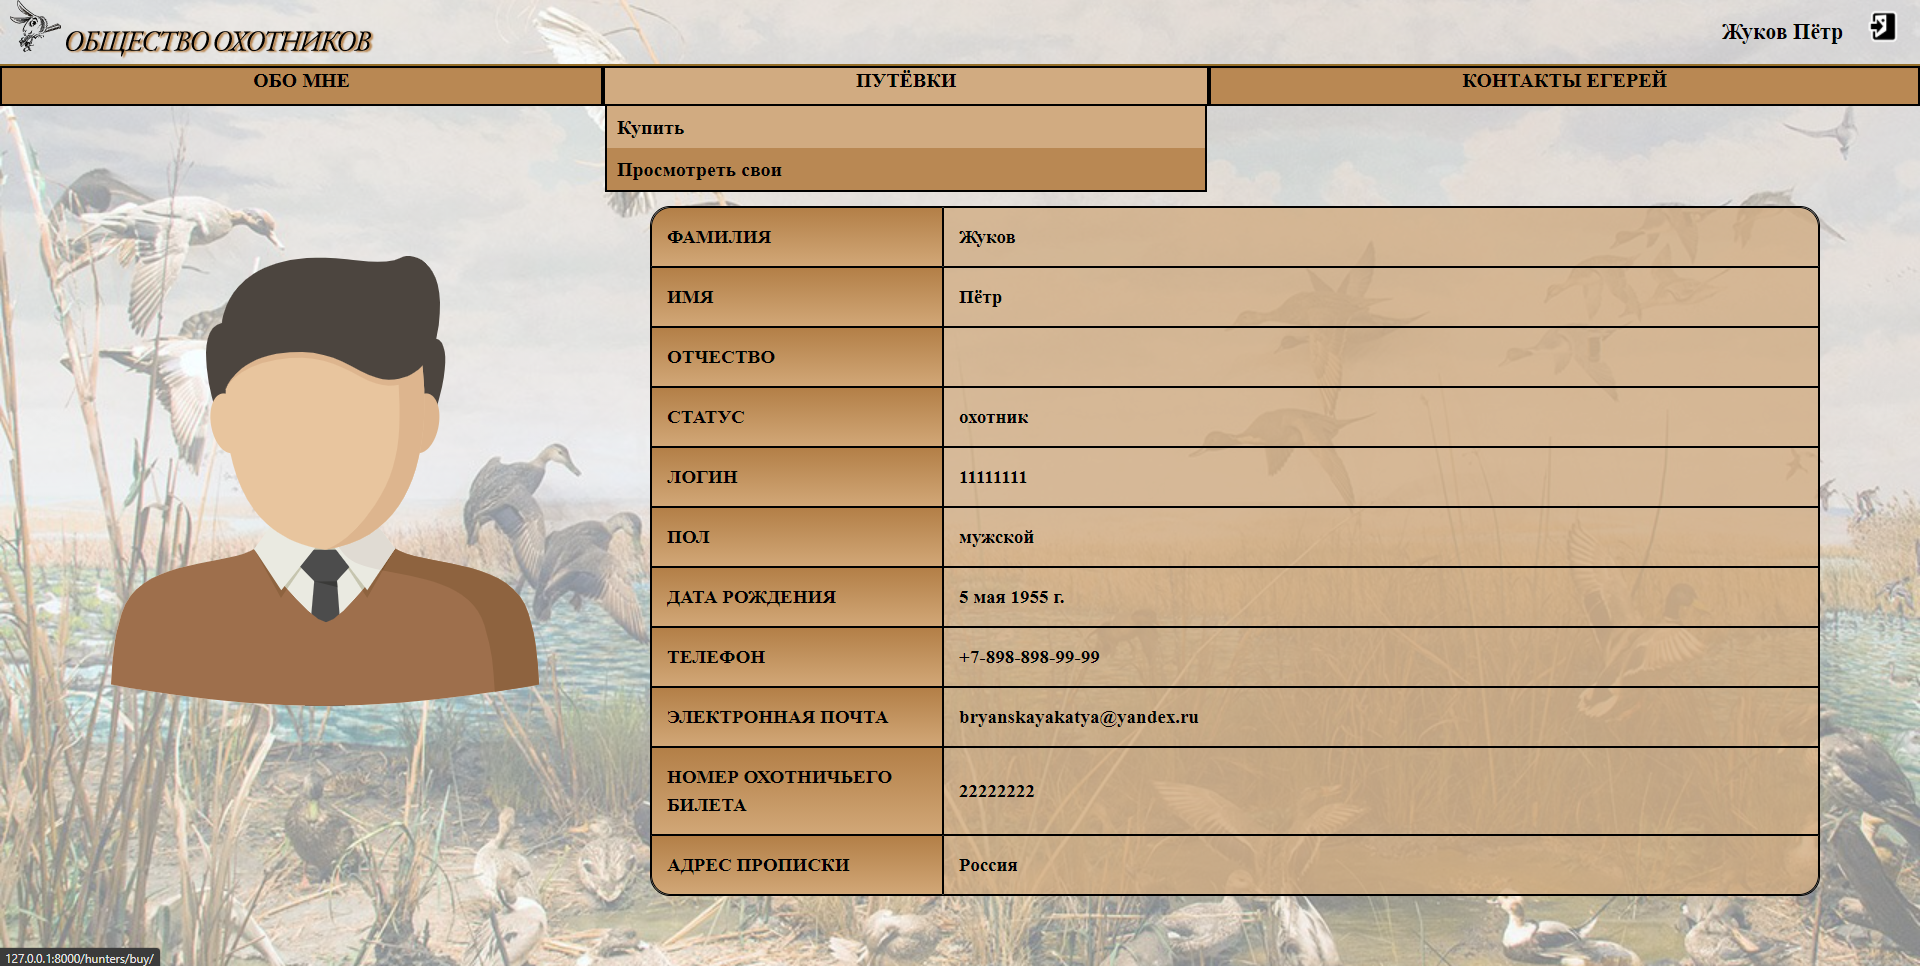
\includegraphics[scale=0.34]{schemes/screens/start.png}}
			\caption{Переход на страницу подачи заявки на путёвку}
			\label{fig10:image}
		\end{center}
	\end{figure}

	После этого охотник попадает на страницу, изображенную на рисунке \ref{fig11:image}. На ней приведён полный список всех доступных путёвок по всем хозяйствам и секторам. Используя мышь или правую полосу прокрутки можно ознакомиться со всем списком. 
	
	Каждая позиция из списка содержит информацию о месте (название хозяйства) и номере сектора, названии животного, на которого выдаётся разрешение, и цена за 1 единицу. 
	
	В поле <<Количество>> пользователь может указать, на сколько животных он хотел бы оформить путёвку. Для этого достаточно нажать кнопкой мыши на это поле в соответствующей строке из прайс-листа. Пользователь может указать число от 1 до 99, причём чтобы контролировать число отстреленных животных только егерь, закрепленный за данным сектором, или администратор может принимать решение одабривать такую заявку или, наоборот, отклонить. 
	
	\begin{figure}[h]
		\centering
		\begin{center}
			{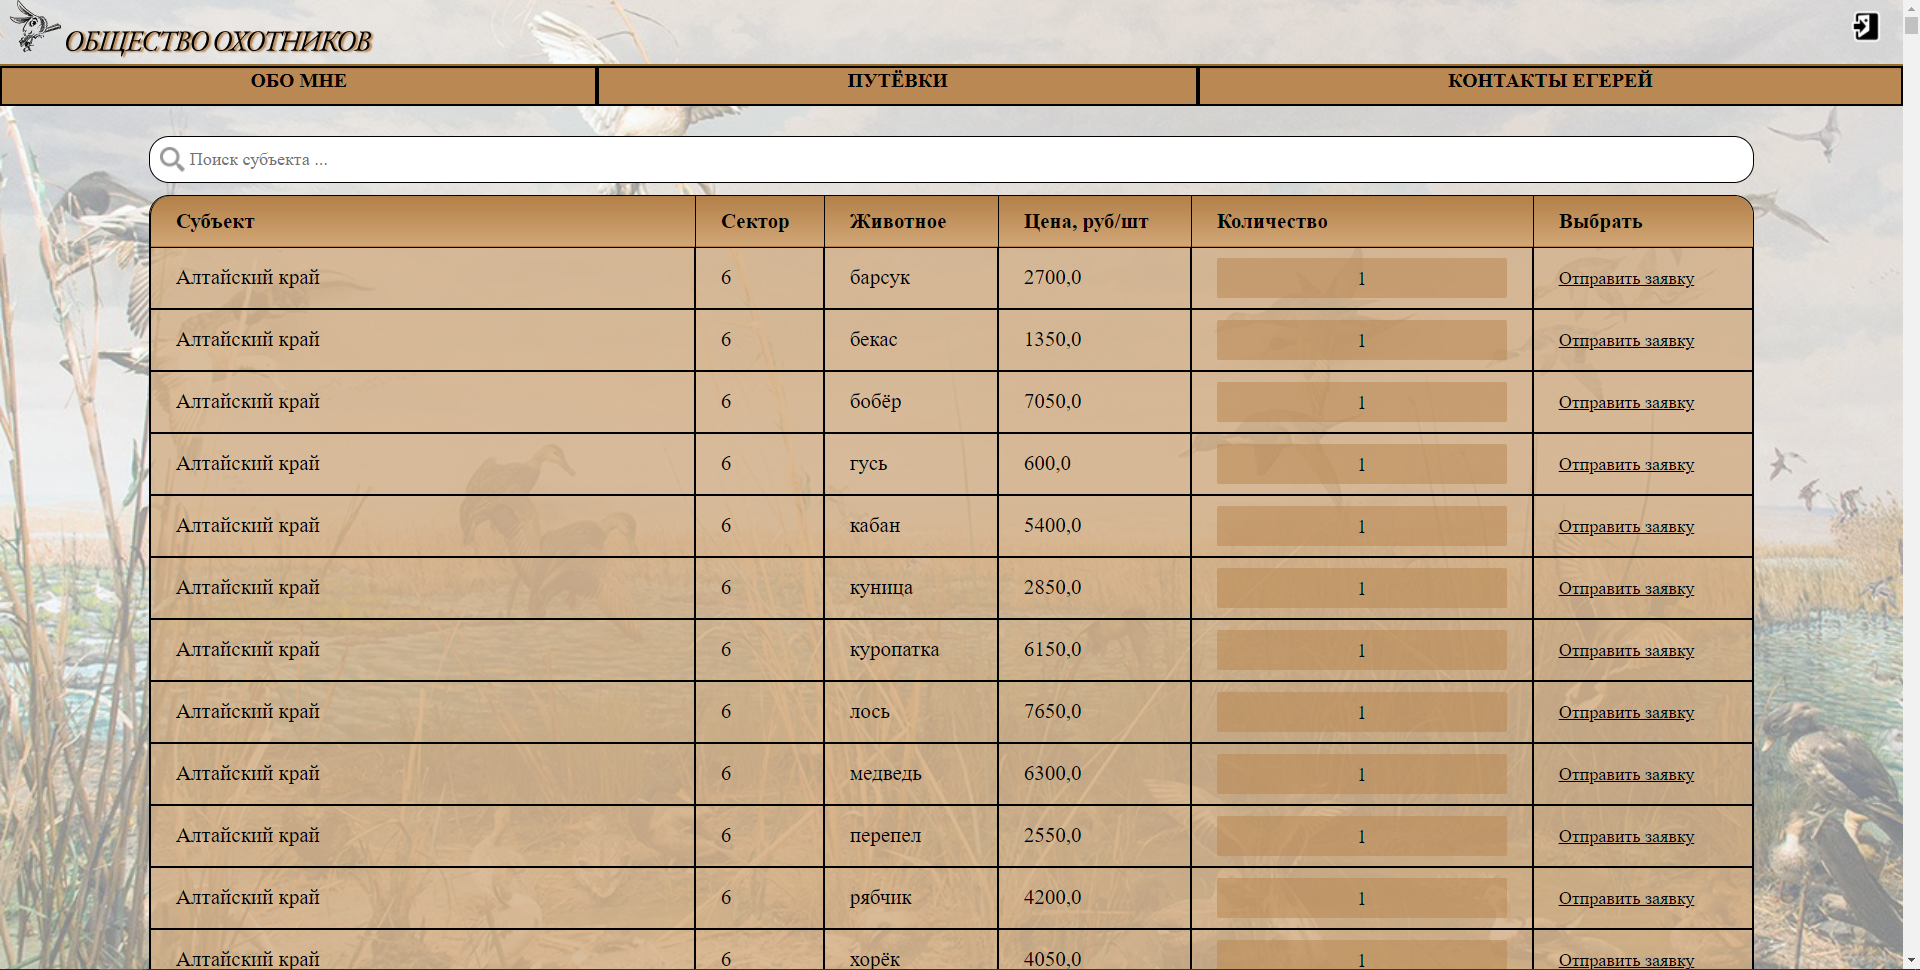
\includegraphics[scale=0.34]{schemes/screens/menu.png}}
			\caption{Прайс-лист доступных путёвок}
			\label{fig11:image}
		\end{center}
	\end{figure}

	Если охотник введёт некорректные данные (например, как на рисунке \ref{fig12:image}) и попробует оформить путёвку, нажав на <<Отправить заявку>>, то он увидит сообщение о невалидности данных (рисунок \ref{fig13:image}).
	
	\begin{figure}[h]
		\centering
		\begin{center}
			{
\includegraphics[scale=0.34]{schemes/screens/wrong_num.png}}
			\caption{Некорректный ввод данный в поле <<Количество>>}
			\label{fig12:image}
		\end{center}
	\end{figure}

	\begin{figure}[h]
		\centering
		\begin{center}
			{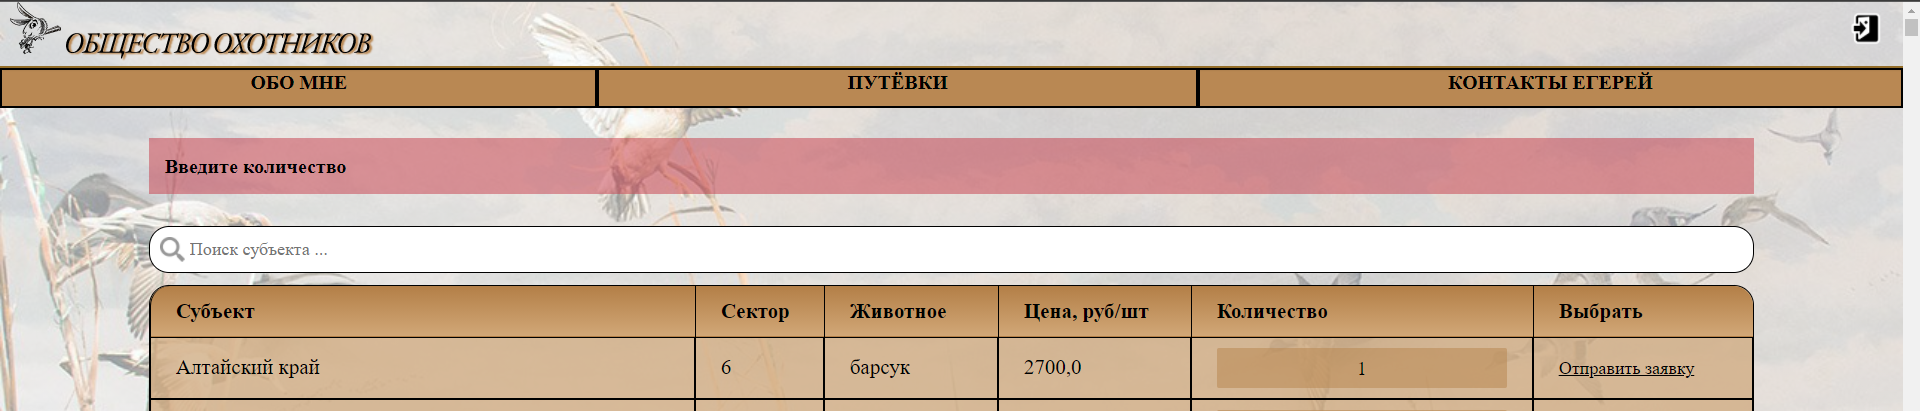
\includegraphics[scale=0.34]{schemes/screens/msg_error.png}}
			\caption{Сообщение о некорректном вводе данных}
			\label{fig13:image}
		\end{center}
	\end{figure}
	\newpage
	
	Также пользователь может воспользоваться поиском по названию субъекта (рисунок \ref{fig14:image}).
	
	\begin{figure}[h]
		\centering
		\begin{center}
			{
\includegraphics[scale=0.3245]{schemes/screens/find.png}}
			\caption{Демонстрация работы поиска}
			\label{fig14:image}
		\end{center}
	\end{figure}
	\newpage

	Если же охотник ввёл корректное число животных (рисунок \ref{fig15:image}) и нажал на <<Отправить заявку>>, то в этом случае на странице появляется соответствующее сообщение, как на рисунке \ref{fig16:image}.
	
	\begin{figure}[h]
		\centering
		\begin{center}
			{
\includegraphics[scale=0.34]{schemes/screens/right_data.png}}
			\caption{Корректно оформленная заявка}
			\label{fig15:image}
		\end{center}
	\end{figure}

	\begin{figure}[h]
		\centering
		\begin{center}
			{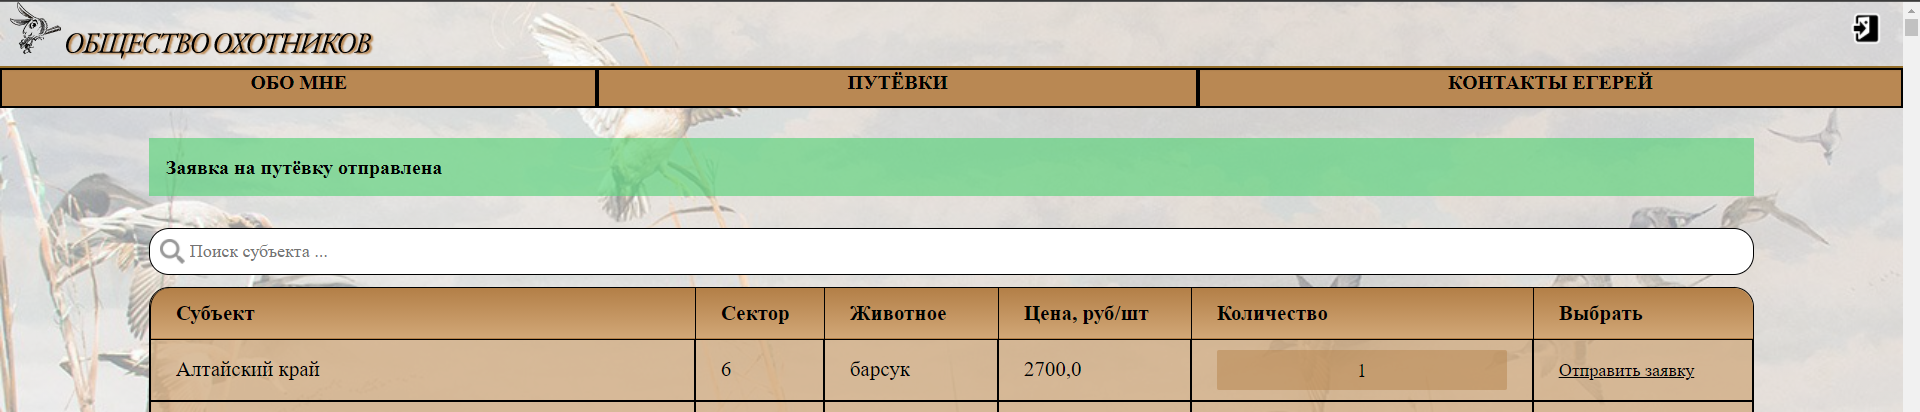
\includegraphics[scale=0.34]{schemes/screens/msg_right.png}}
			\caption{Сообщение об успешном оформлении заявки}
			\label{fig16:image}
		\end{center}
	\end{figure}

	Просмотреть все свои заявки, а также уже одобренные путёвки охотник может, кликнув на поле <<Просмотреть свои>> (рисунок \ref{fig17:image}).
	
	\begin{figure}[h]
		\centering
		\begin{center}
			{
\includegraphics[scale=0.34]{schemes/screens/to_have.png}}
			\caption{Переход на страницу всех заявок и одобренных путёвок}
			\label{fig17:image}
		\end{center}
	\end{figure}

	В результате охотник попадает на страницу, изображённую на рисунке \ref{fig18:image}. На ней сначала указаны все одобренные текущему охотнику путёвки (то есть, по ним он уже может охотиться), и ниже все заявки. Также по каждой из этих двух таблиц можно осуществить поиск по субъекту. На рисунке \ref{fig15:image} указано, какая именно позиция из прайс-листа была выбрана, и уже на этой странице можно увидеть эту заявку (выделена белым цветом).
	
	\begin{figure}[h]
		\centering
		\begin{center}
			{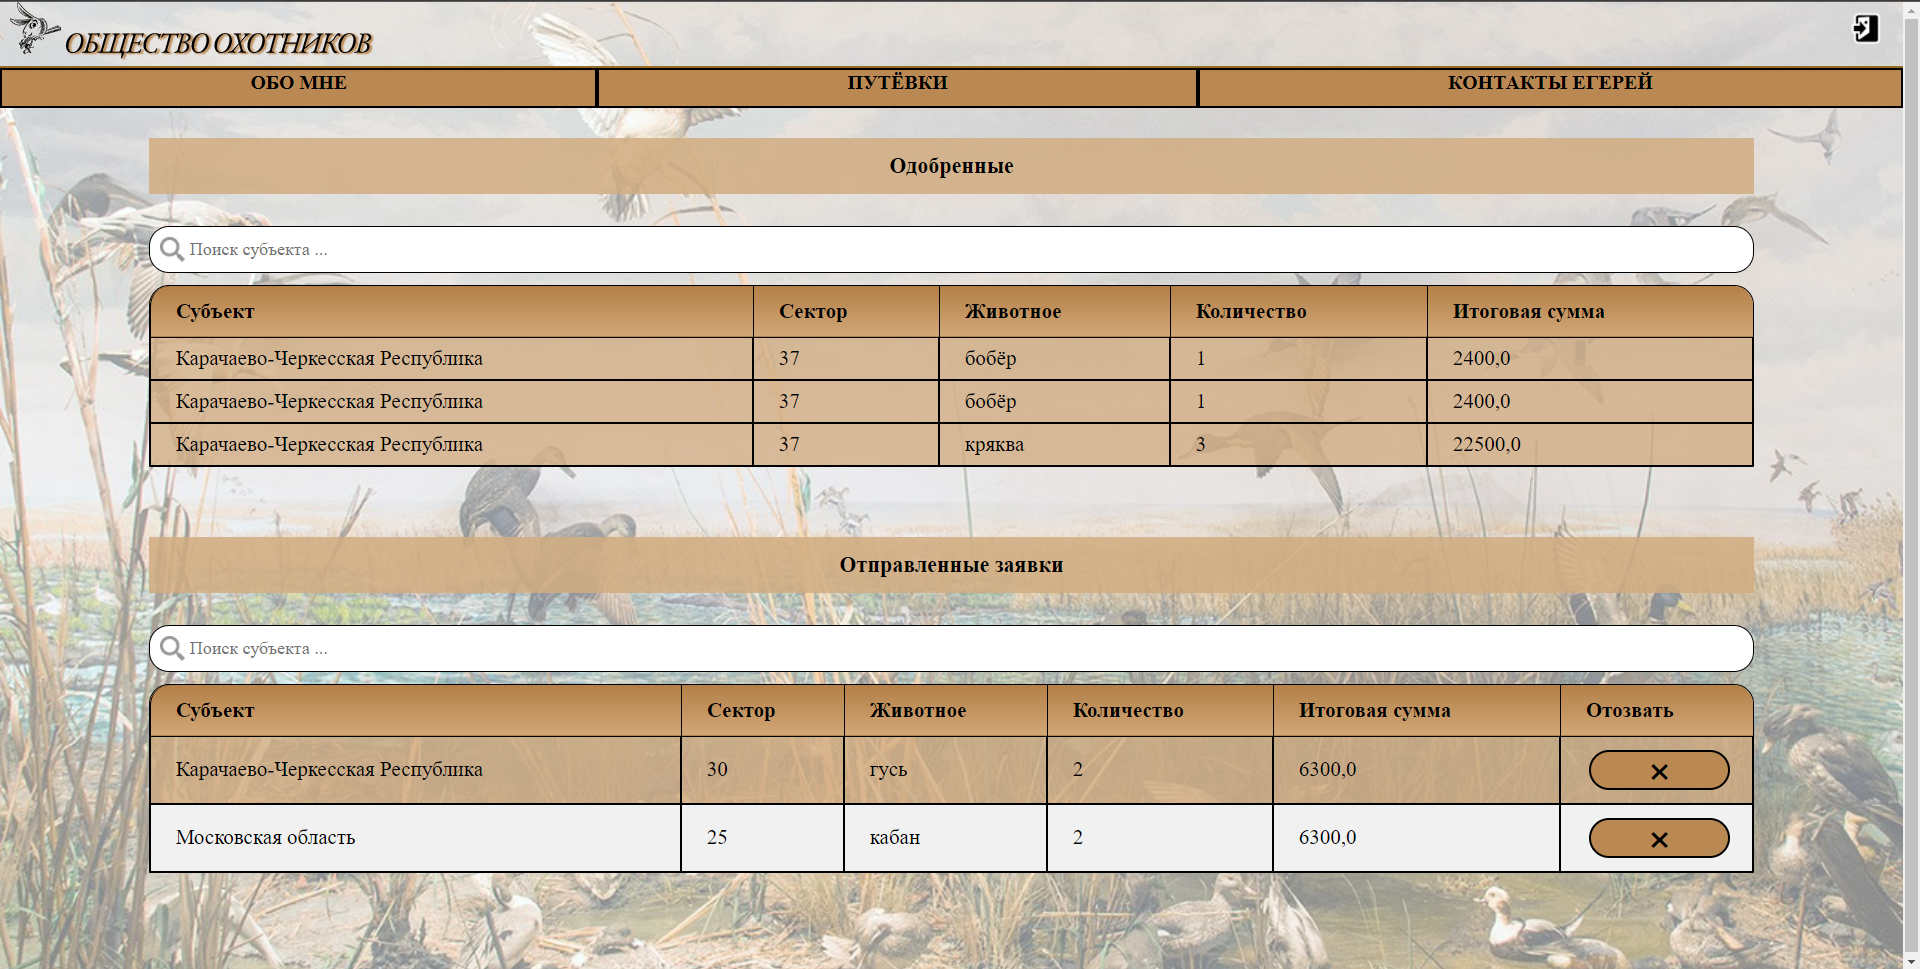
\includegraphics[scale=0.34]{schemes/screens/all_vouchers.png}}
			\caption{Всех заявки и одобренные путёвок текущего охотника}
			\label{fig18:image}
		\end{center}
	\end{figure}

	Если по какой-то причине пользователь передумал оформлять путёвку, то он может отозвать оформленную ранее заявку, нажав на кнопку в столбце <<Отозвать>>. 
	
	Для наглядности была отозвана путёвка на гуся. После этого страница выглядит так, как показано на рисунке \ref{fig19:image}. 
	
	Показателем того, что операция прошла успешно, является соответствующее сообщение и отсутствие выбранной позиции на странице. 
	
	Удалить или отозвать уже одобренные путёвки охотник не может, так как считается, что покупка уже совершена, а закрыть её по определённым причинам может только егерь, закреплённый за сектором, куда была выдана путёвка, или администратор.
	
	\begin{figure}[pt!]
		\centering
		\begin{center}
			{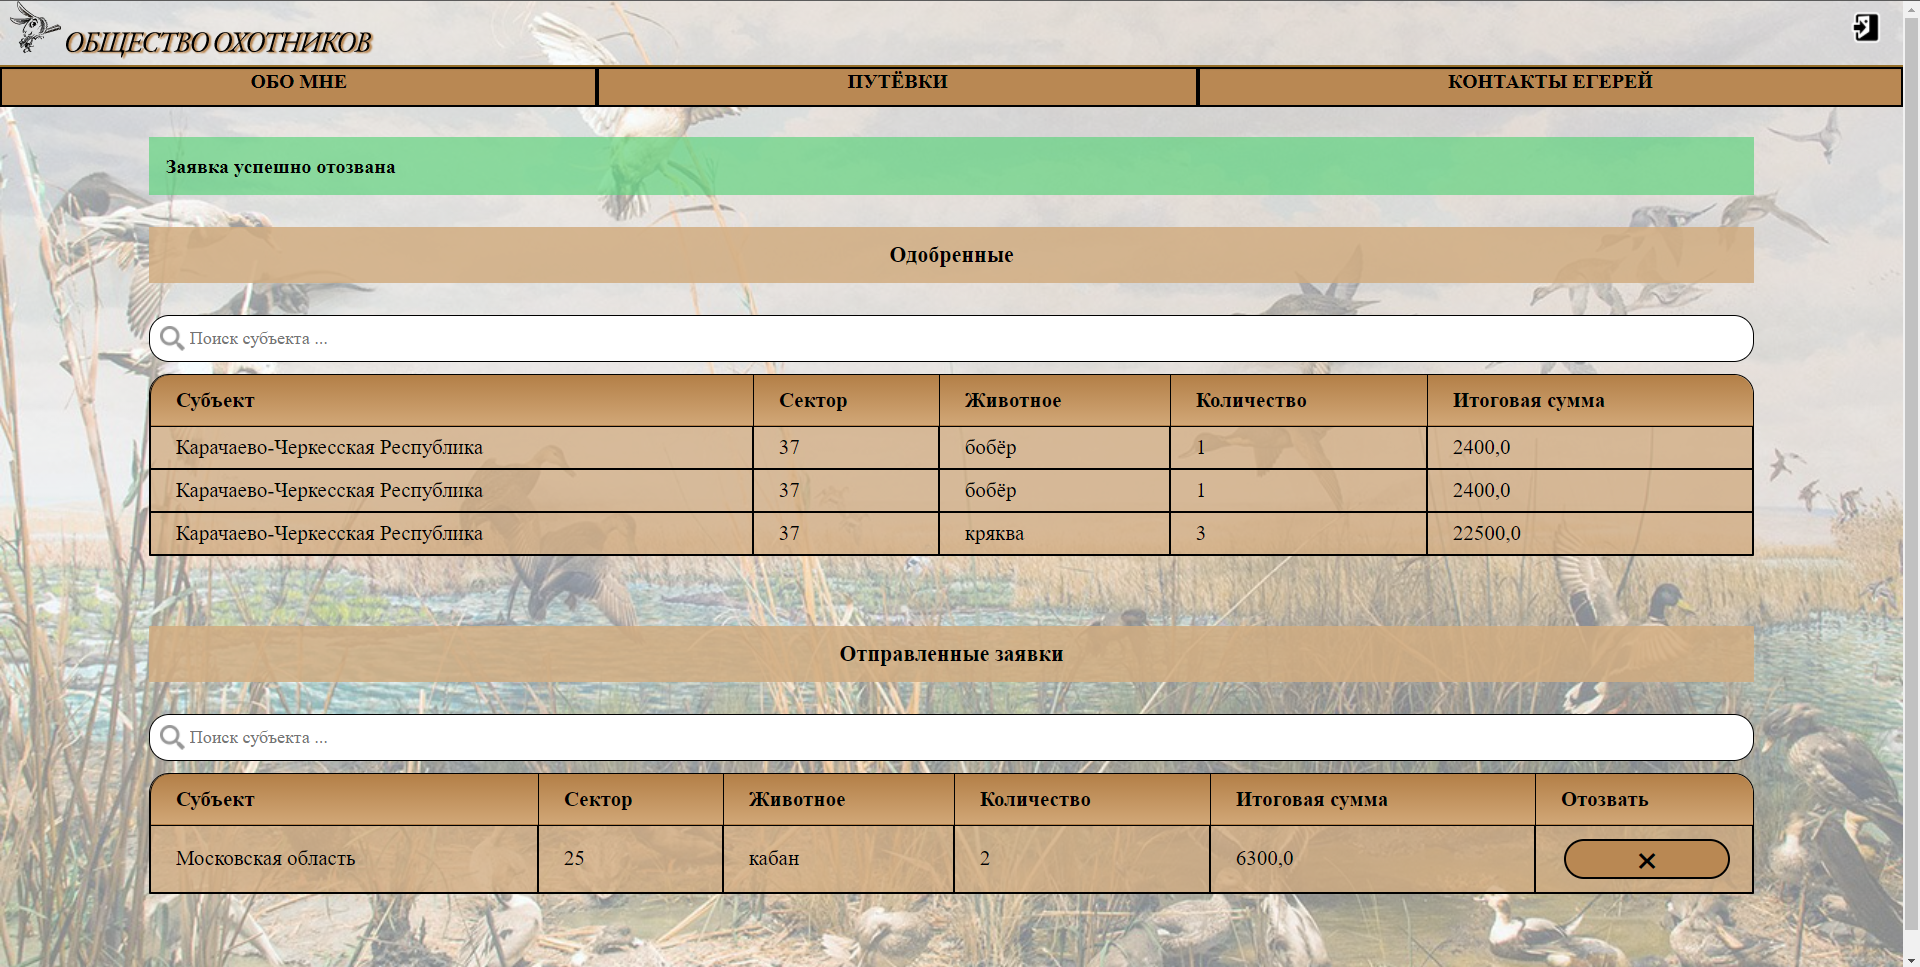
\includegraphics[scale=0.34]{schemes/screens/after_del_huntsman.png}}
			\caption{Страница после того, как была отозвана заявка}
			\label{fig19:image}
		\end{center}
	\end{figure}
	\newpage

	Также оперировать заявками на охоту и путёвками может и егерь. Для того, чтобы просмотреть заявки ему также нужно перейти по тому же пункту меню (рисунок \ref{fig20:image}). Стоит отметить, что видеть и проводить какие-либо операции егерь может только над теми заявками и путёвками, которые были оформлены в его хозяйство и сектор, к остальным данным он доступа не имеет.
	
	\begin{figure}[h]
		\centering
		\begin{center}
			{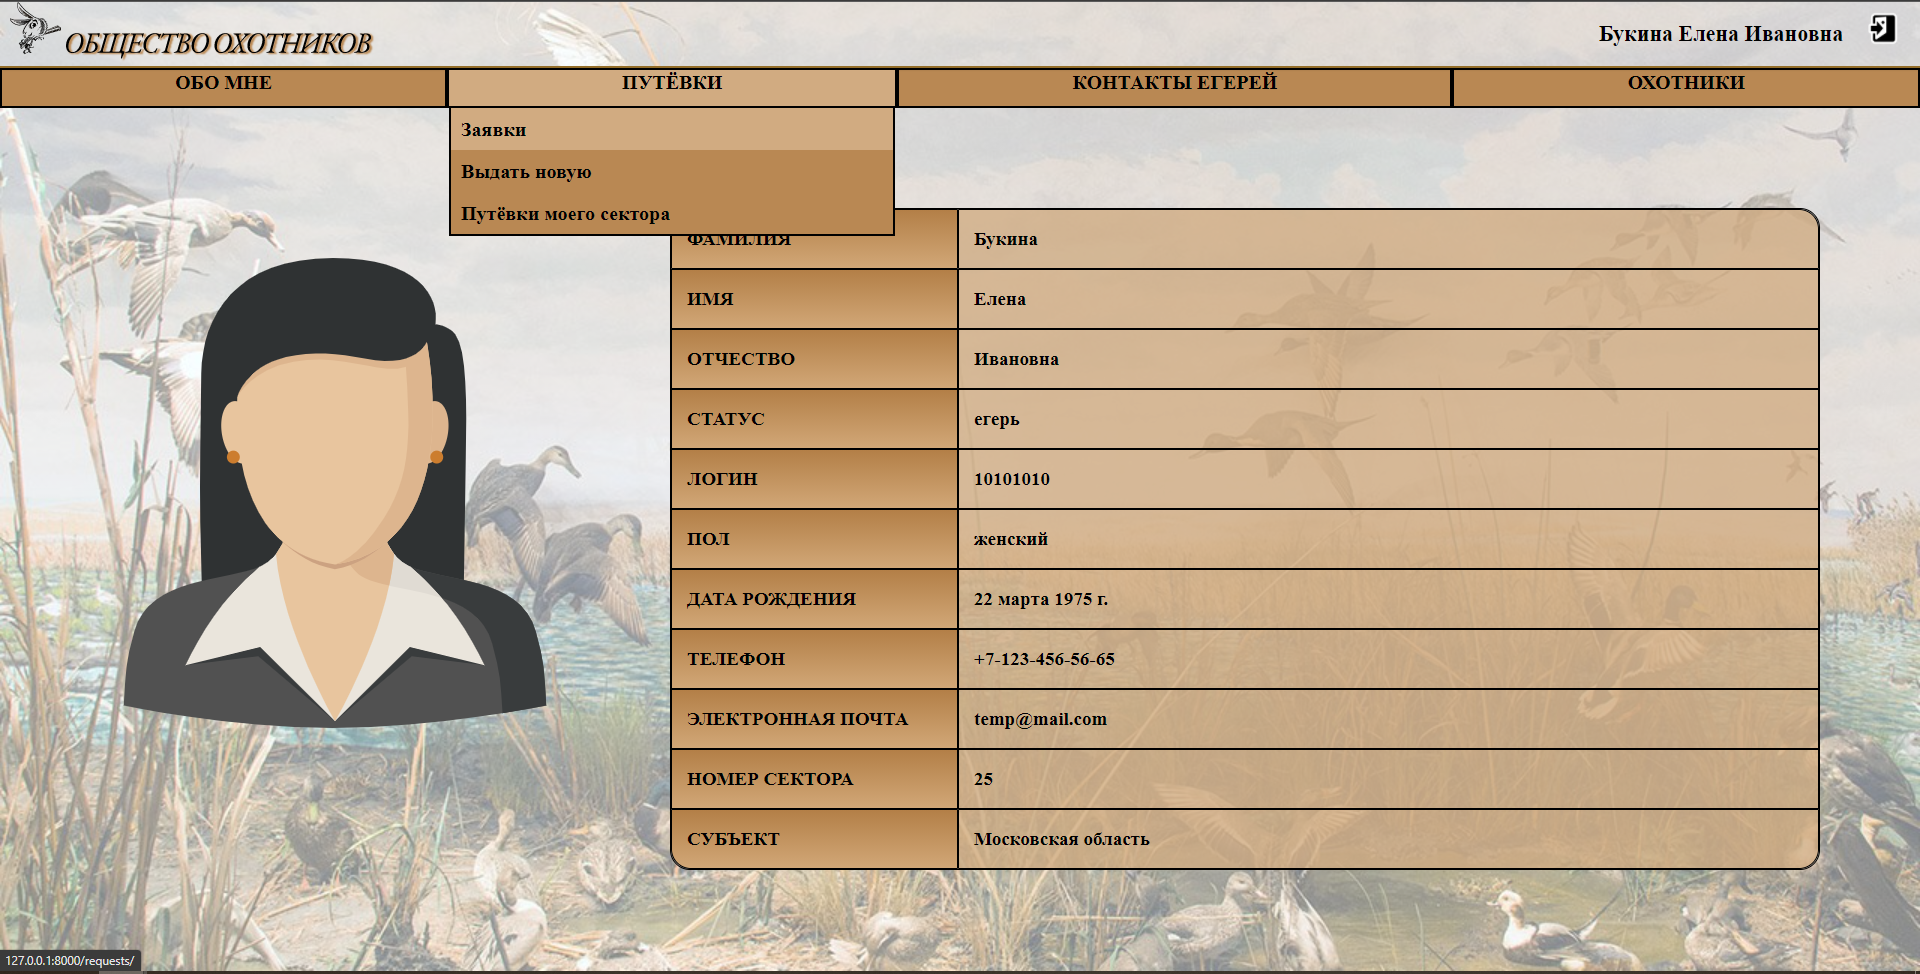
\includegraphics[scale=0.34]{schemes/screens/huntsman_start.png}}
			\caption{Переход на страницу заявок со стороны егеря}
			\label{fig20:image}
		\end{center}
	\end{figure}
	\newpage

	Страница заявок изображена на рисунке \ref{fig21:image}. Белым цветом выделена путёвка, которая оформлялось ранее. Егерь может как одобрить путёвку, нажав на <<галочку>>, так и отклонить, выбрав <<крестик>>. Также егерю предоставляется поиск по ФИО.

	\begin{figure}[h]
		\centering
		\begin{center}
			{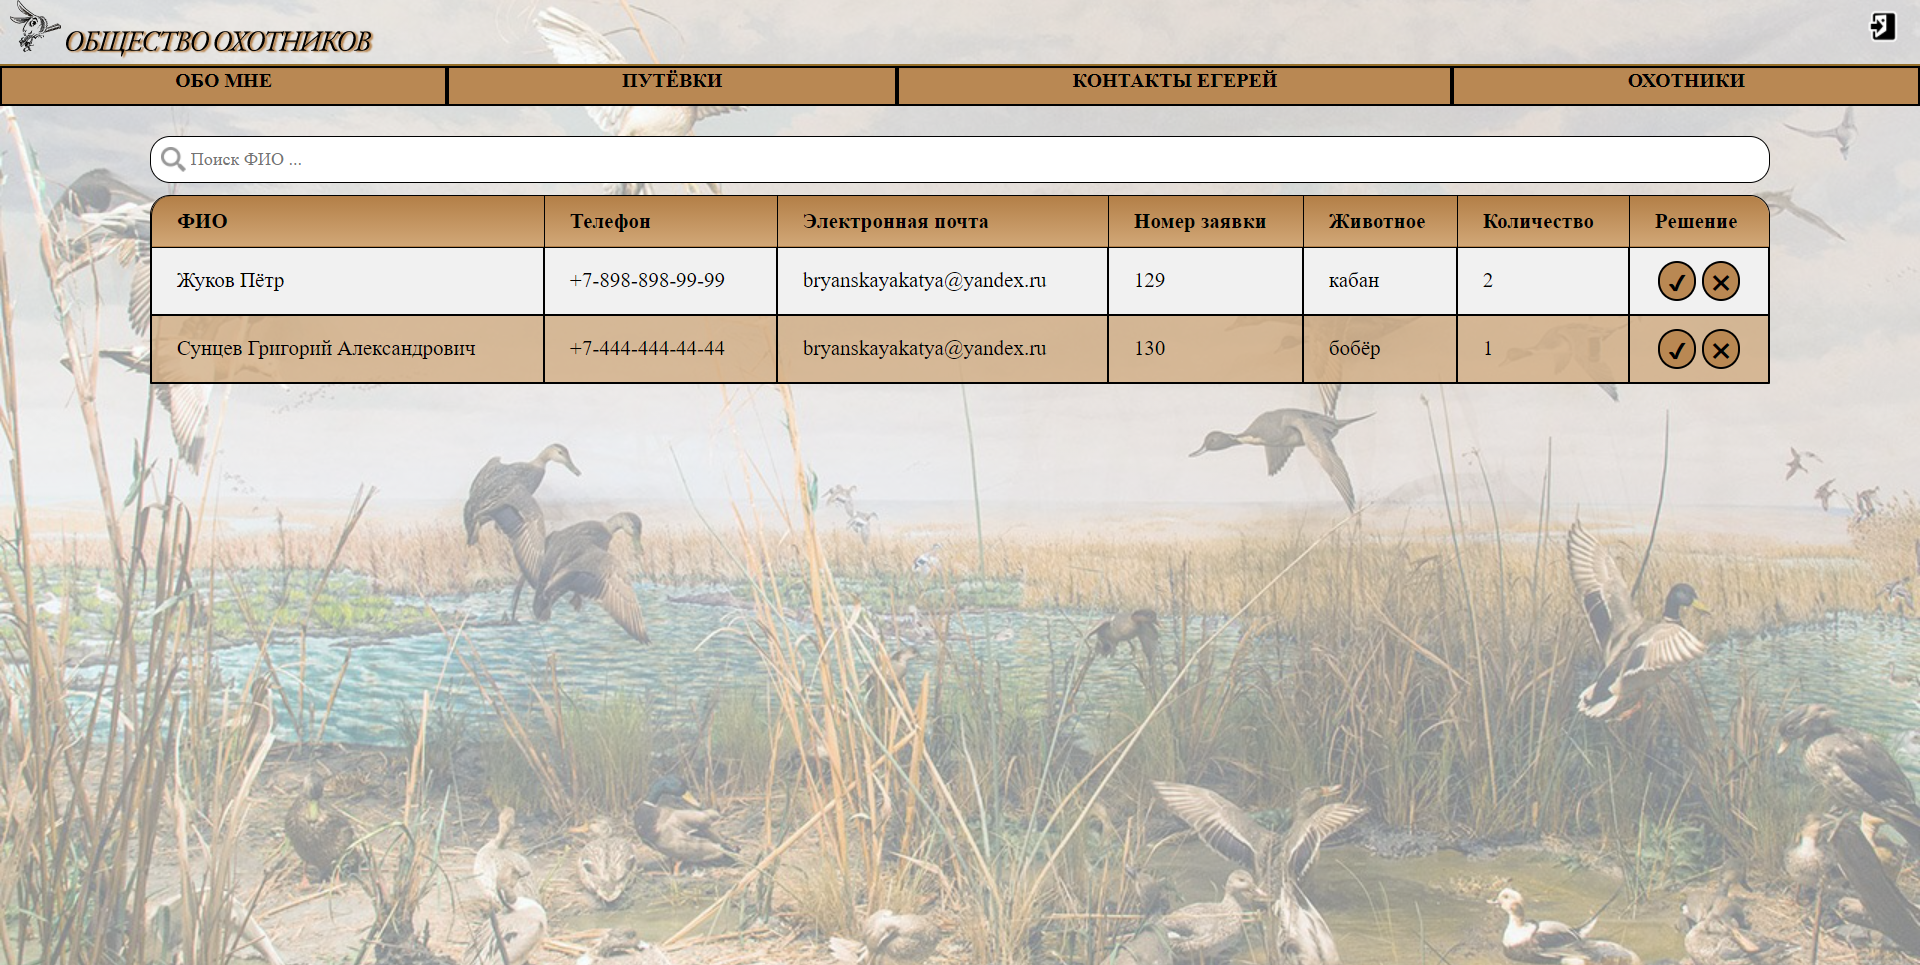
\includegraphics[scale=0.321]{schemes/screens/requests_huntsman.png}}
			\caption{Страница заявок, доступных егерю}
			\label{fig21:image}
		\end{center}
	\end{figure}

	Перейдя по пункту <<Путёвки моего сектора>> из меню (рисунок \ref{fig20:image}) на страницу, изображённую на рисунке \ref{fig23:image}, пользователь получает соответствующий список.
	
	\begin{figure}[h]
		\centering
		\begin{center}
			{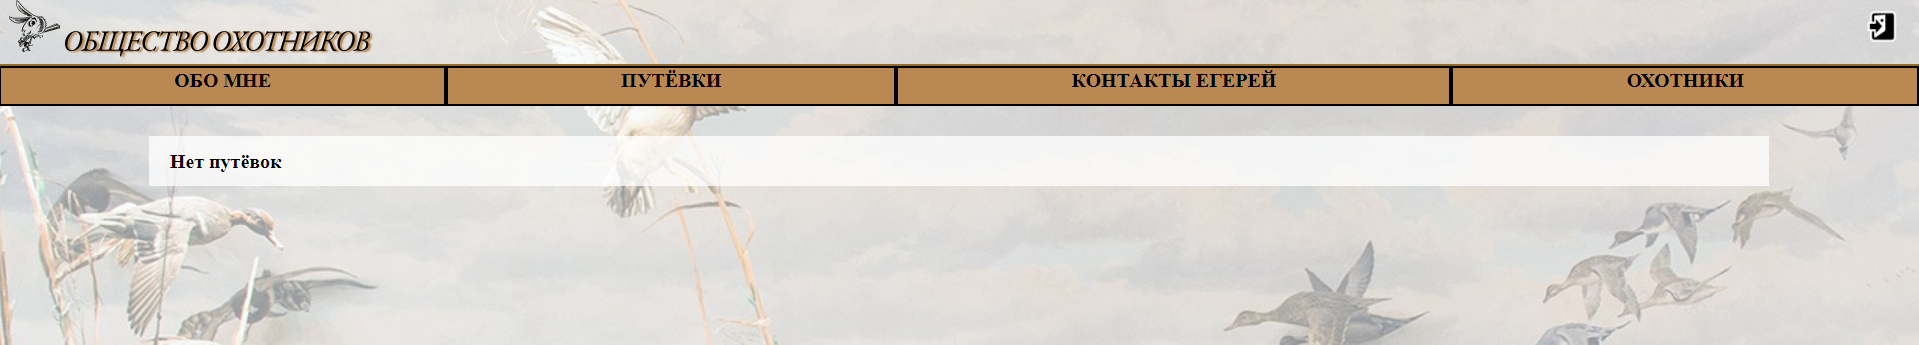
\includegraphics[scale=0.34]{schemes/screens/vouchers_huntsman2.png}}
			\caption{Страница одобренных путёвок, доступных егерю}
			\label{fig23:image}
		\end{center}
	\end{figure}
	\newpage

	На данный момент выданных путёвок нет. Если егерь примет решение одобрить путёвку на кабана (рисунок \ref{fig21:image}) и нажмёт <<галочку>>, то страницы заявок (рисунок \ref{fig24:image}) и путёвок (рисунок \ref{fig25:image}) примут соответствующий вид.
	
	\begin{figure}[h!]
		\centering
		\begin{center}
			{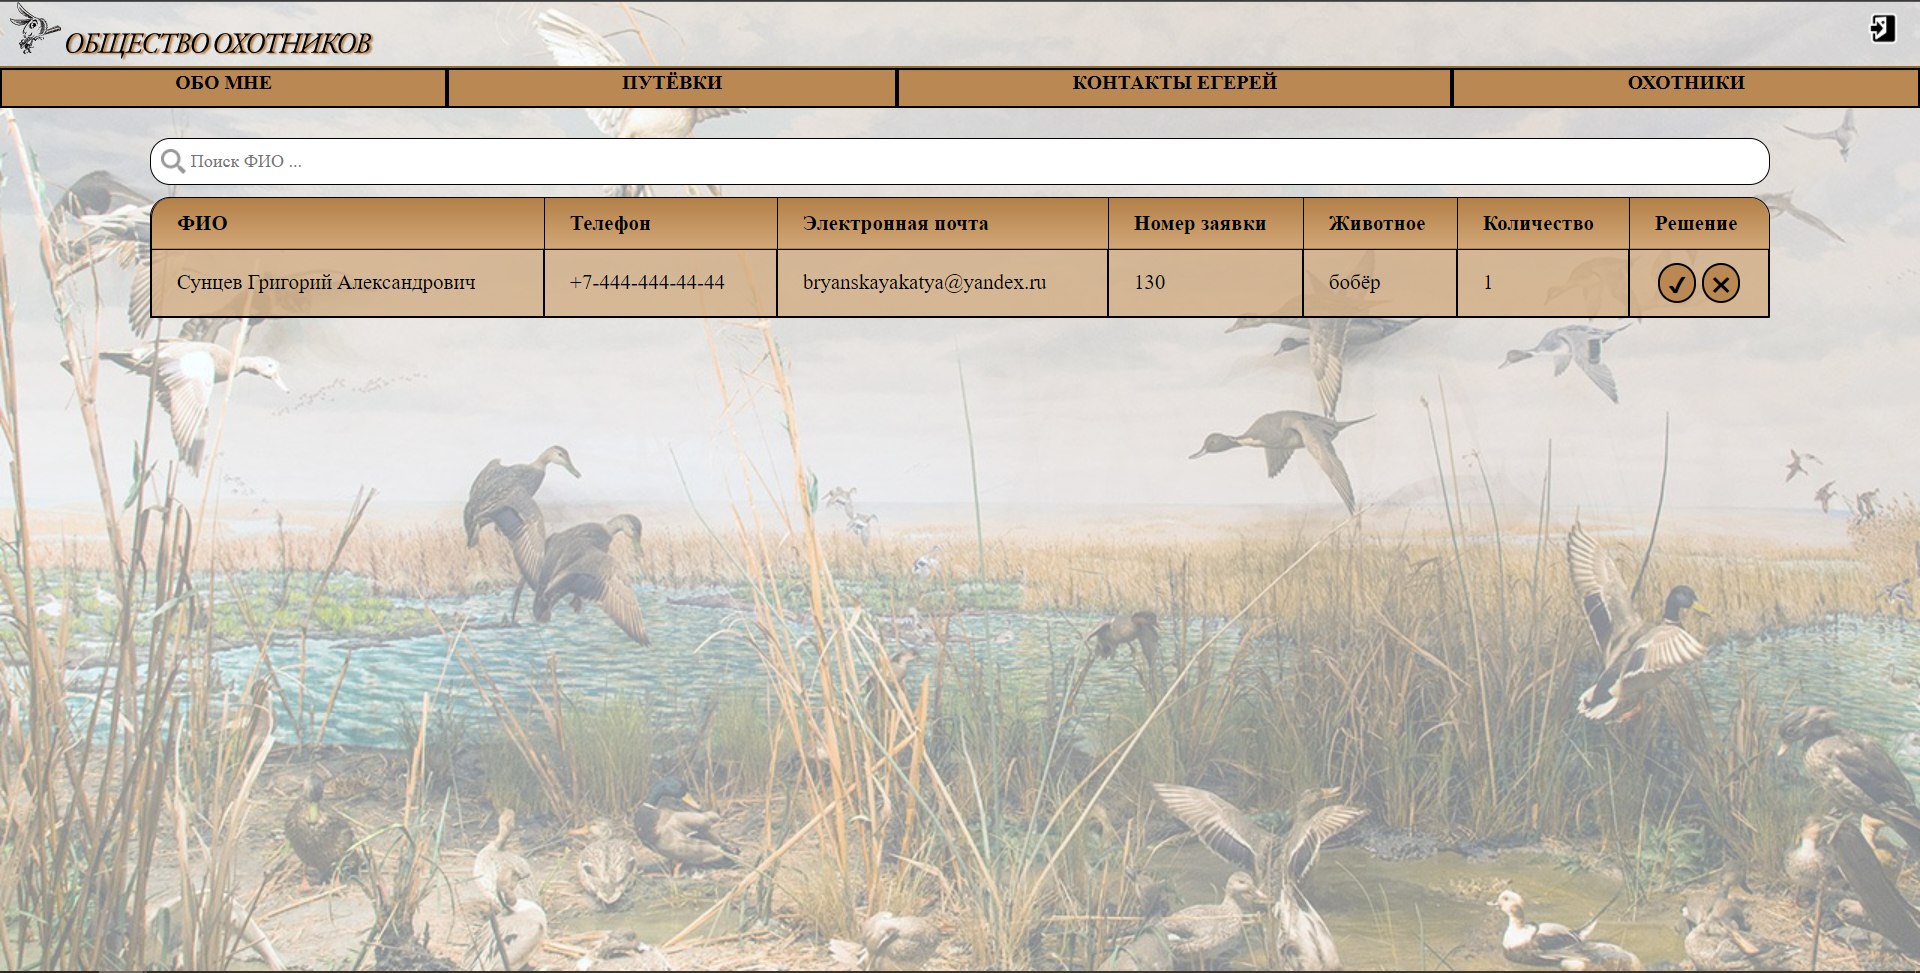
\includegraphics[scale=0.34]{schemes/screens/requests_huntsman_add.png}}
			\caption{Страница заявок, доступных егерю, после одобрения}
			\label{fig24:image}
		\end{center}
	\end{figure} 

	\begin{figure}[pt!]
		\centering
		\begin{center}
			{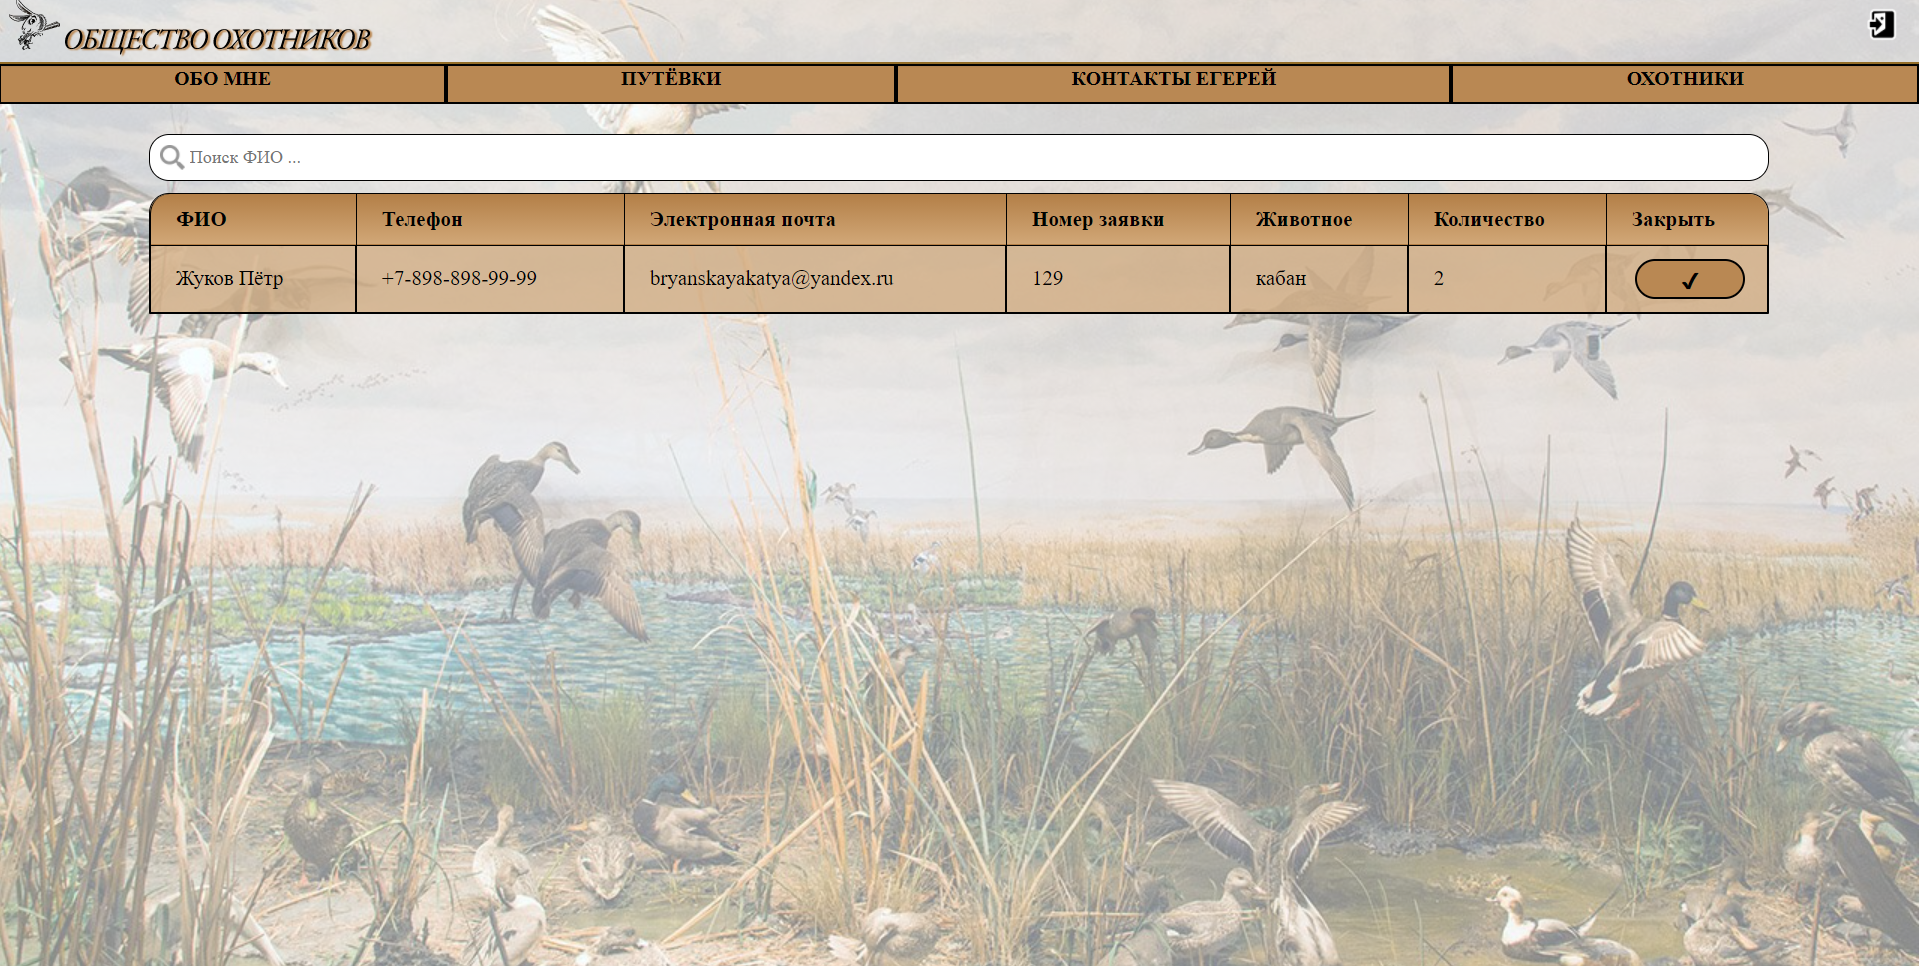
\includegraphics[scale=0.34]{schemes/screens/vouchers_huntsman_add.png}}
			\caption{Страница одобренных путёвок, доступных егерю, после одобрения}
			\label{fig25:image}
		\end{center}
	\end{figure} 
	\newpage

	Оформленная ранее путёвка теперь числится не в ожидающий заявках, а в одобренных путёвках.
	
	Егерь также может закрыть путёвку (например, при её истечении), для этого он должен нажать на соответствующую кнопку в столбце <<Закрыть>> на странице путёвок (рисунок \ref{fig25:image}), и данная позиция перестанет существовать.
	
	Егерь также может принять решение об отказе на оформление путёвки, для этого он нажимает <<крестик>> (рисунок \ref{fig24:image}). В такой ситуации путёвка пропадёт не только у егеря, но и у охотника, на чьё имя она была оформлена.\\

	Помимо этого егерь может выдать кому-то путёвку, но только в то хозяйствой и сектор, к которому прикреплён сам. В таком случае, оформленная путёвка сразу получает статус одобренной и попадает в соответствующий раздел. Чтобы перейти на страницу оформления путёвки, нужно выбрать пункт <<Выдать новую>> из меню (рисунок \ref{fig20:image}). Егерь в таком случае попадает на страницу, приведённую на рисунке \ref{fig28:image}.

	\begin{figure}[h]
		\centering
		\begin{center}
			{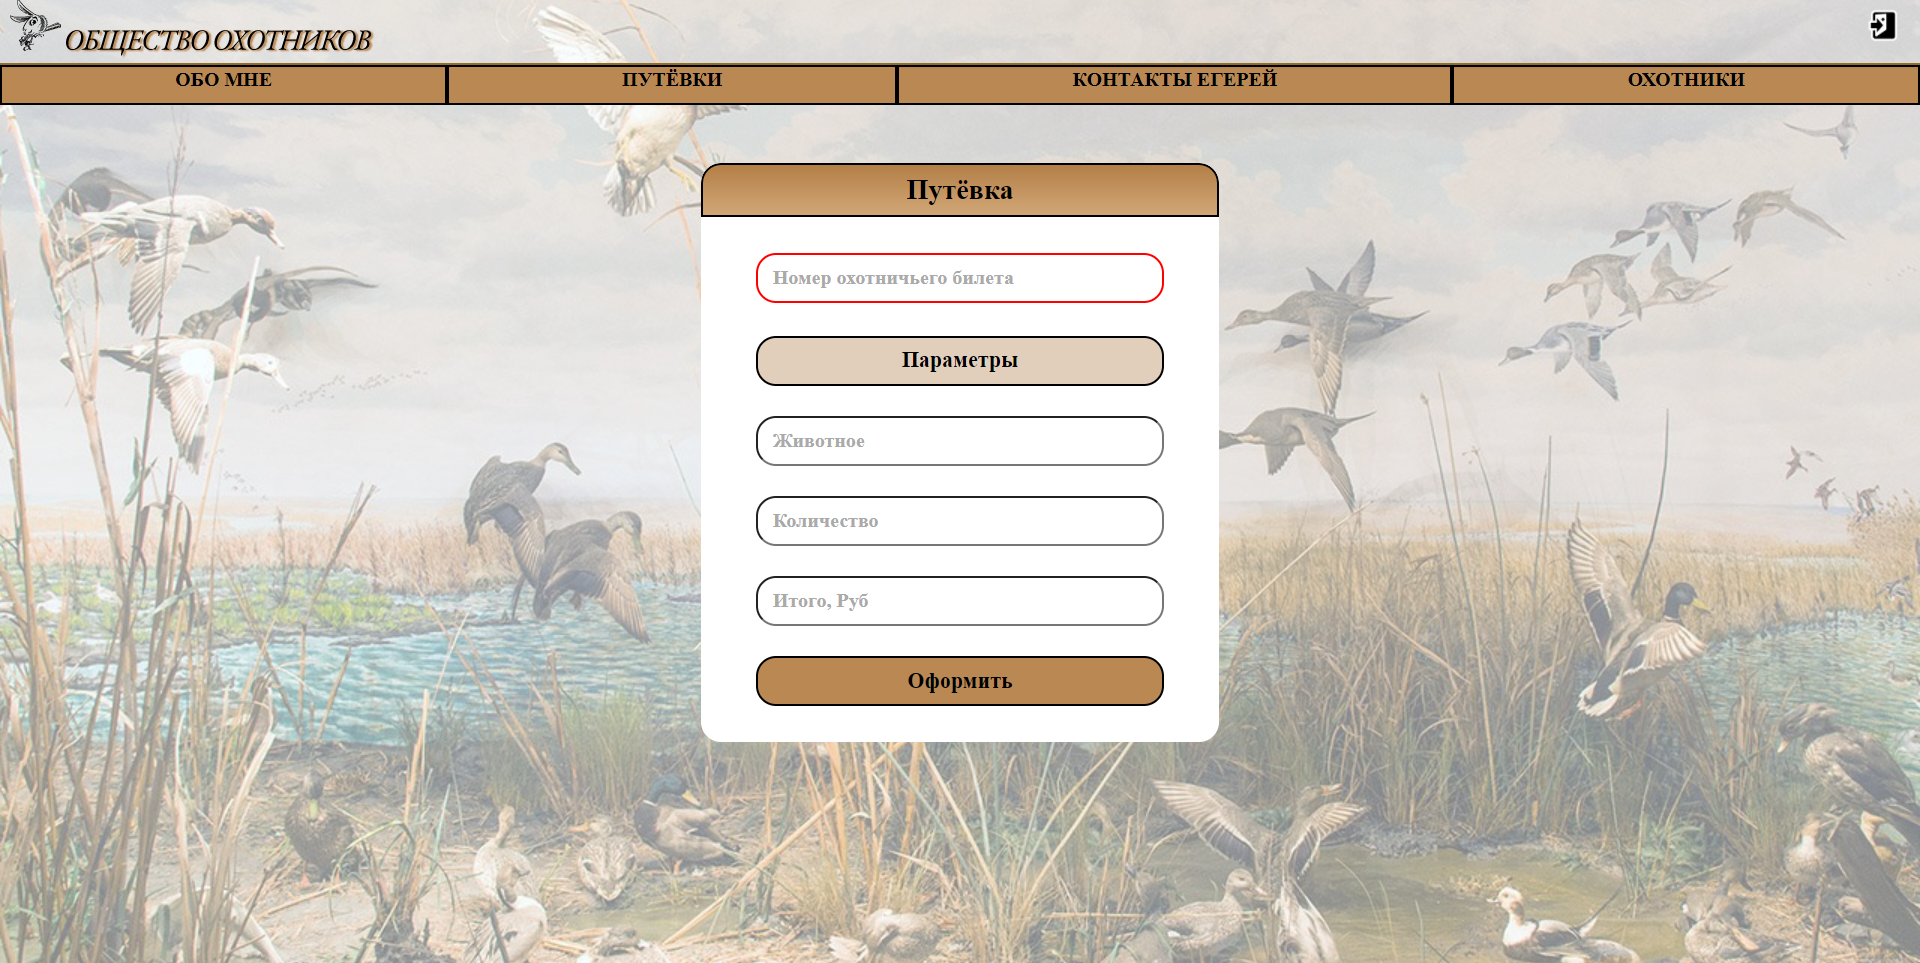
\includegraphics[scale=0.34]{schemes/screens/create_huntsman.png}}
			\caption{Оформление путёвки егерем}
			\label{fig28:image}
		\end{center}
	\end{figure}
	\newpage

	Помимо поля, предназначенного для ввода номера охотничьего билета, необходимо также выбрать параметры. Делается это по нажатию на одноимённую кнопку. В результате егерю предоставляется весь прайс-лист, действующий в его секторе (рисунок \ref{fig29:image}).
	
	\begin{figure}[h!]
		\centering
		\begin{center}
			{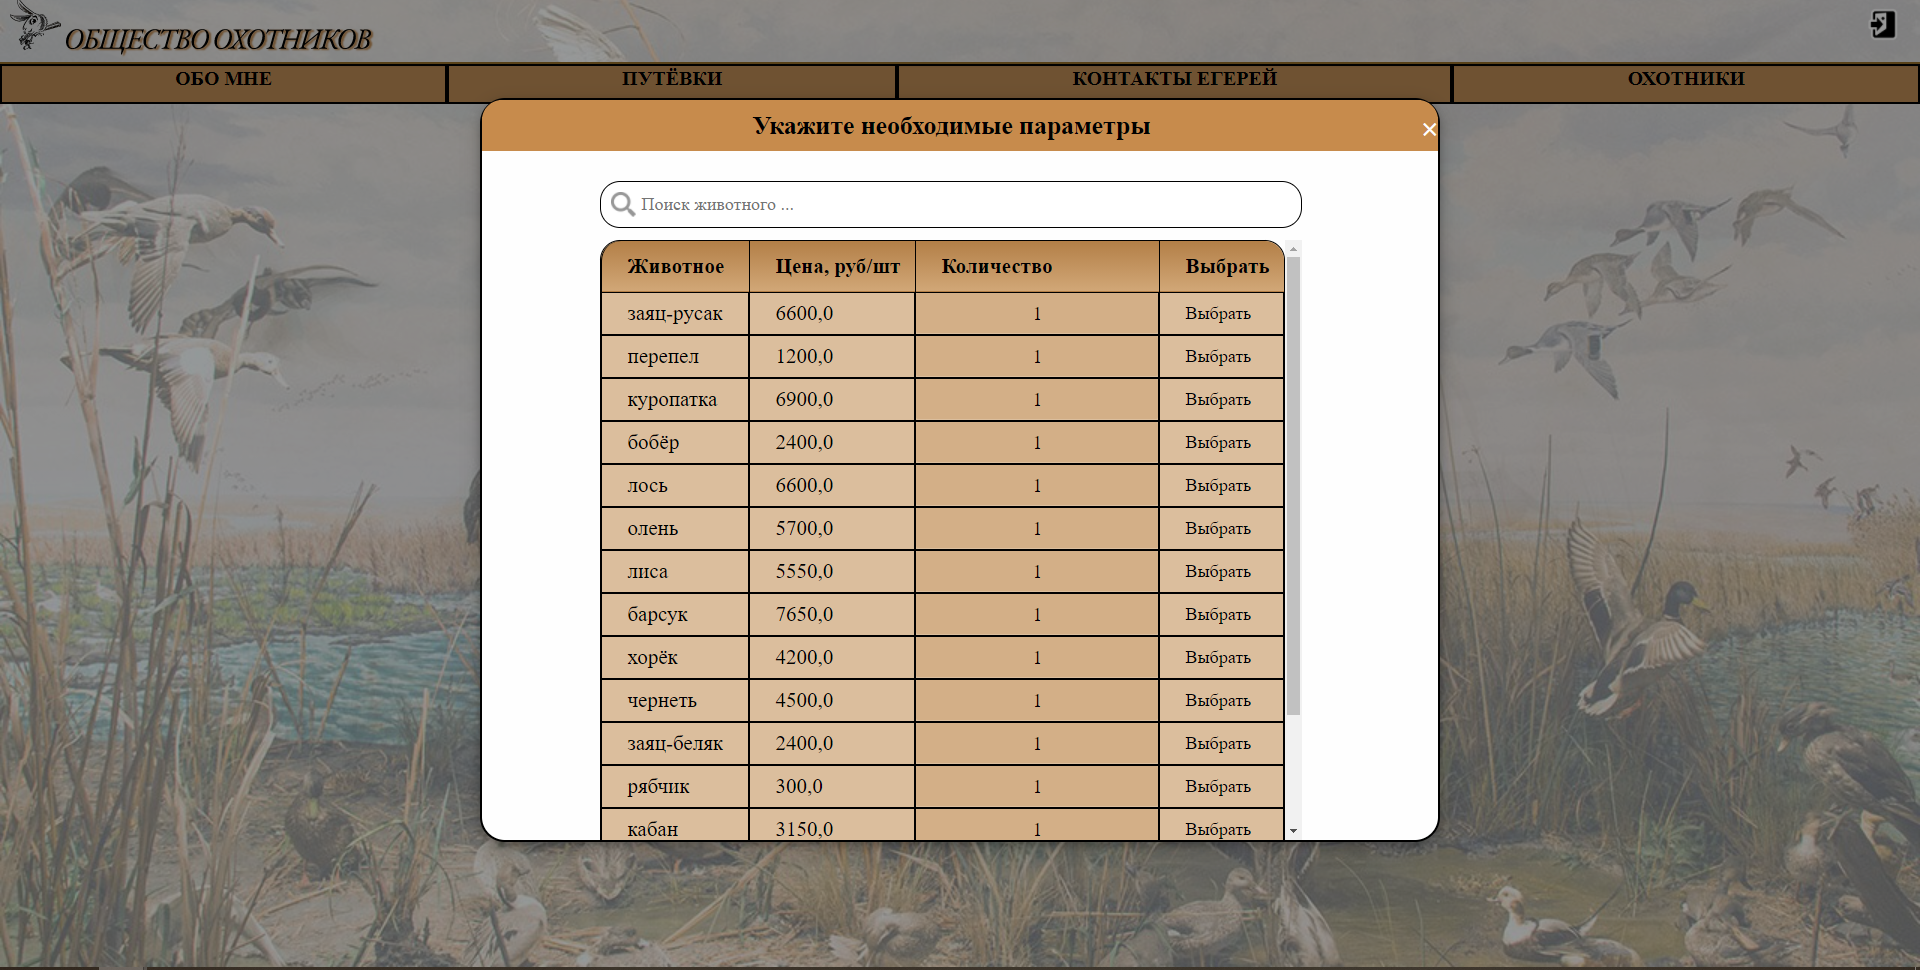
\includegraphics[scale=0.34]{schemes/screens/price_list_huntsman.png}}
			\caption{Выбор параметров путёвки}
			\label{fig29:image}
		\end{center}
	\end{figure}

	Здесь также предусмотрен поиск по названию животного, а также проверка на валидность введенного количества, аналогичная той, что была ранее.
	
	Заполнив поля (рисунок \ref{fig28:image}) и нажав кнопку <<Оформить>> может возникнуть одна из двух ситуаций. Первая - когда всё верно, и в базе действительно существует охотник с указанным билетом, в таком случае, егерь просто попадает на страницу разрешённых путёвок и наблюдает там только что оформленную путёвку. И вторая - охотника с таким номером нет, в таком случае, просто выводится ошибка на экран.
	
	Что касается администратора, то он может выполнять те же операции над заявками и путёвками, что и егерь, с той лишь разницей, что ему предоставляются данные со всех хозяйств и секторов. Так, страницы заявок (рисунок \ref{fig31:image}) и одобренных путёвок (рисунок \ref{fig32:image}) со стороны администратора отличаются только наличием столбцов о месте проведения, функционал такой же.
	
	\begin{figure}[h!]
		\centering
		\begin{center}
			{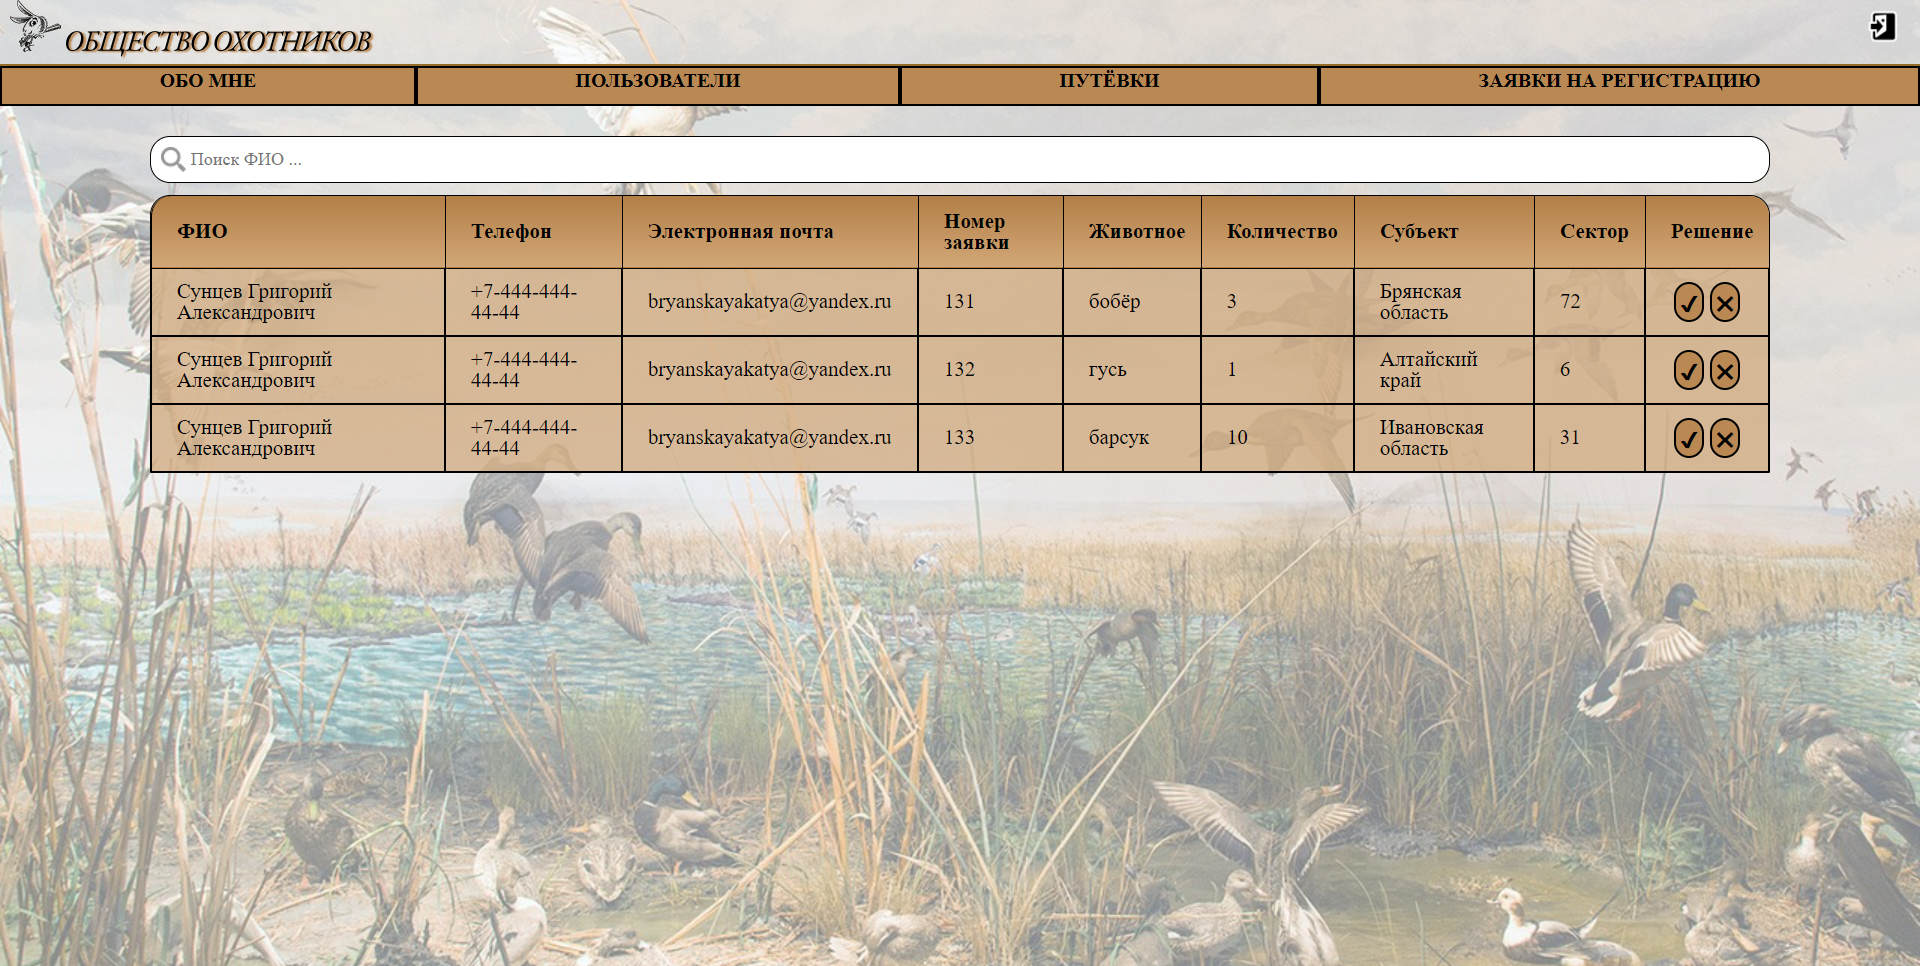
\includegraphics[scale=0.34]{schemes/screens/requests_admin.png}}
			\caption{Страница заявок со стороны администратора}
			\label{fig31:image}
		\end{center}
	\end{figure}

	\begin{figure}[h!]
		\centering
		\begin{center}
			{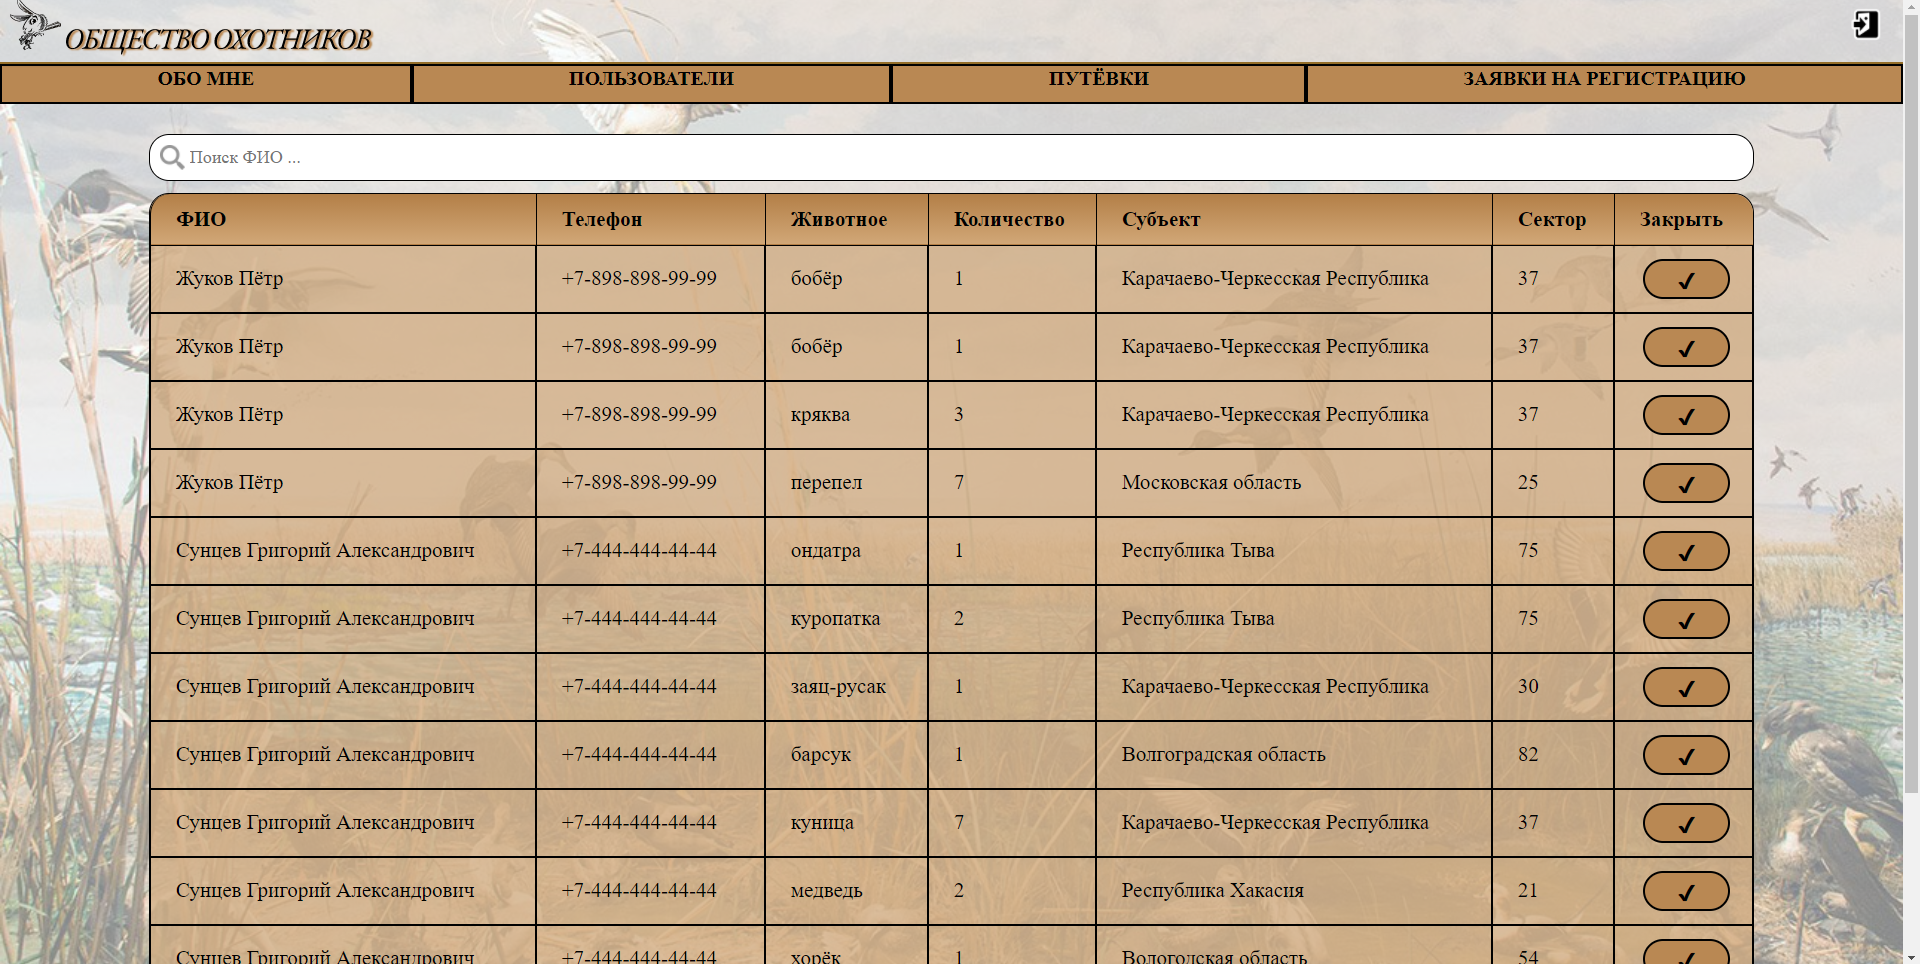
\includegraphics[scale=0.34]{schemes/screens/vouchers_admin.png}}
			\caption{Страница одобренных путёвок со стороны администратора}
			\label{fig32:image}
		\end{center}
	\end{figure}
	\newpage

	Возможность оформления путёвки через администратора тоже есть, он также должен заполнить форму, аналогичную изображенной на рисунке \ref{fig28:image}, только теперь  ещё надо заполнить поле о месте проведения (рисунок \ref{fig33:image}).
	
	\begin{figure}[h!]
		\centering
		\begin{center}
			{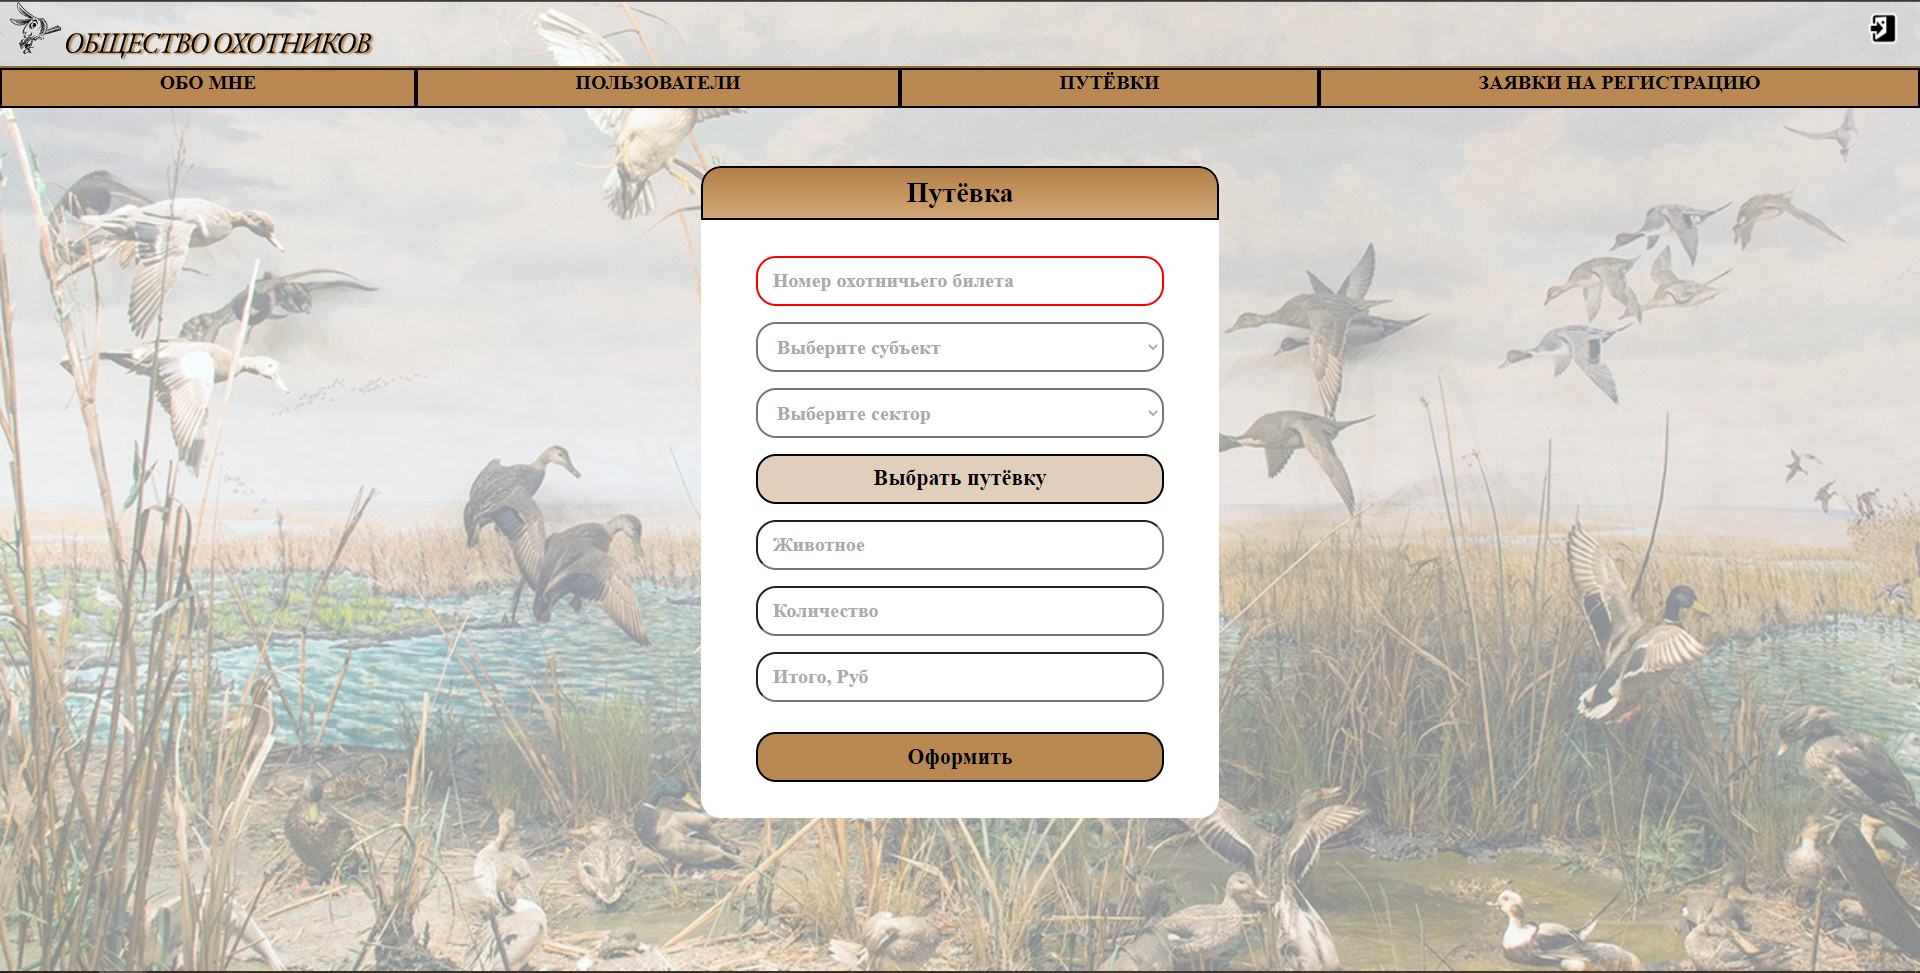
\includegraphics[scale=0.34]{schemes/screens/create_admin.png}}
			\caption{Оформление путёвки администратором}
			\label{fig33:image}
		\end{center}
	\end{figure}
	\newpage

	Поля <<Выберите субъект>> и <<Выберите сектор>> представляют из себя выпадающие списки (рисунок \ref{fig34:image}). Это сделано для того, чтобы минимизировать количество вводимых с клавиатуры данных, с целью сократить число возникающих в ходе заполнения ошибок.
	
	\begin{figure}[h!]
		\centering
		\begin{center}
			{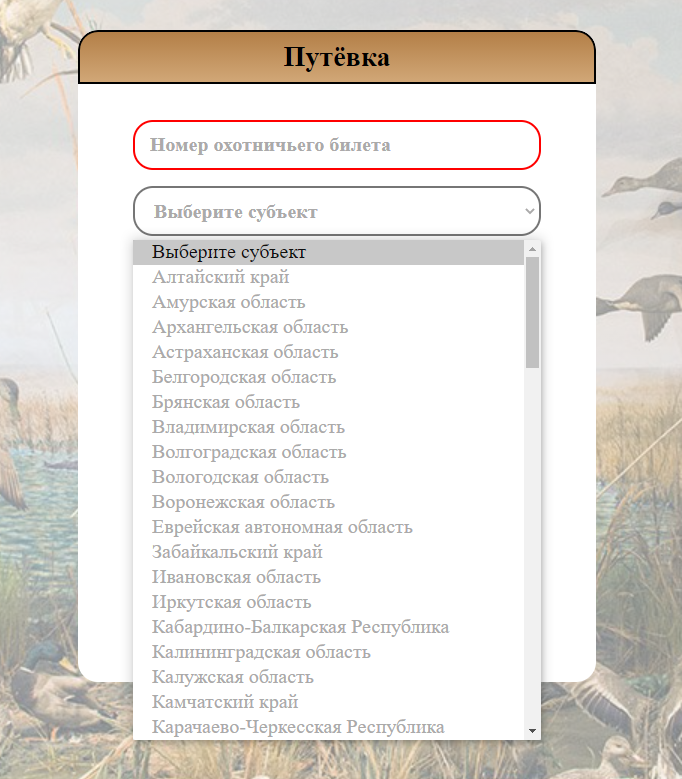
\includegraphics[scale=0.5]{schemes/screens/scroll_menu.png}}
			\caption{Выпадающий список}
			\label{fig34:image}
		\end{center}
	\end{figure}
	
	\subsection*{Вывод}
	Для реализации поставленной задачи были выбраны язык программирования Python и среды разработки Pycharm и Visual Studio Code.
	
	В качестве используемых СУБД и ORM были выбраны PostgreSQL и peewee, а для разработки приложения - Web-фреймворк Django.
	
	В разделе также были представлены в виде UML-диаграмм компонент доступа к данным, компонент бизнес-логики, представления, а также общая диаграмма приложения.
	
	Был также освещён интерфейс приложения, задействованный при оформлении разными ролями путёвки на охоту.
	
	
	
	
	










	
	
		
		 
		
	
	\newpage
	
	\section*{Заключение}
\addcontentsline{toc}{section}{Заключение}
	В ходе написания курсового проекта была достигнута поставленная цель, а именно, спроектирована и реализована база данных для <<Общества охотников>>, а также разработано Web-приложение для взаимодействия с ней.
	
	В процессе её выполнения были решены все задачи: проведён анализ существующих решений, на его основе было формализовано задание и определён функционал. Помимо этого были рассмотрены различные СУБД с целью выбора наиболее подходящей для решения поставленной задачи. Была спроектирована и заполнена база данных, и разработано Web-приложение, взаимодействующее с ней.


	\newpage
	
	\newpage
	\begin{thebibliography}{9} 
		\addcontentsline{toc}{section}{Литература}
		
		\bibitem{Russia-in-numbers} \textbf{Россия} в цифрах. 2020: Крат.стат.сб./Россат- М., 2020 - 550 с. ISBN 978-5-89476-488-7.
		
		\bibitem{doc_problems} Распоряжение Правительства Российской Федерации от 03.07.2014 N 1216-р <Об утверждении Стратегии развития охотничьего хозяйства в Российской Федерации до 2030 года> // СПС <<Консультант Плюс>> 2021 
		
		\bibitem{maps} Геопортал охотничьего хозяйства России [Электронный ресурс]. Режим доступа: https://huntmap.ru/ (дата обращения 23.03.2021).
		
		\bibitem{db} Дейт К. Дж. Введение в системы баз данных. — 8-е изд. — М.: «Вильямс», 2006. — 1328 с. — ISBN 0-321-19784-4.
		
		\bibitem{db_systems} Коннолли Т., Бегг К. Базы данных. Проектирование, реализация и сопровождение. Теория и практика — 3-е изд. — М.: Вильямс, 2003. — 1436 с. — ISBN 0-201-70857-4.
		
		\bibitem{NF} Нормализация отношений. Шесть нормальных форм [Электронный ресурс], режим доступа: https://habr.com/ru/post/254773/, свободный (дата обращения: 29.03.2021).
		
		\bibitem{mvc} Джесс Чедвик и др. ASP.NET MVC 4: разработка реальных веб-приложений с помощью ASP.NET MVC — М.: «Вильямс», 2013. — 432 с. — ISBN 978-5-8459-1841-3.
		
		\bibitem{python} Документация Python 3.9.5 [Электронный ресурс]. Режим доступа: https://docs.python.org/3/, свободный (дата обращения: 18.03.2021).

		
		\bibitem{pycharm} PyCharm [Электронный ресурс], режим доступа: https://www.jetbrains.com/ru-ru/pycharm/, свободный (дата обращения:
		18.03.2021).
		
		\bibitem{vcode} Visual Studio Code [Электронный ресурс], режим доступа: https://code.visualstudio.com/ (дата обращения: 27.04.2021).
		
		\bibitem{postgresql} PostgreSQL [Электронный ресурс], режим доступа: https://postgrespro.ru/docs/postgresql (дата обращения: 05.03.21).
		
		\bibitem{peewee} Документация ORM peewee [Электронный ресурс]. Режим доступа: http://docs.peewee-orm.com/en/latest, свободный (дата обращения: 27.03.2021)
		
		\bibitem{django} Документация Web-фреймворка Django [Электронный ресурс].
		Режим доступа: https://docs.djangoproject.com/en/3.2/, свободный (дата обращения: 05.03.2021)
		
		
		
	\end{thebibliography}
	\newpage
	
%	\input{section/introduction.tex}
%	\section{Раздел первый}
%	Немного текста Немного текста Немного текста Немного текста Немного текста Немного текста Немного текста Немного 
	
%	\subsection{ghbdtn}
	
%	текста Немного текста Немного текста Немного текста Немного текста Немного текста Немного текста Немного текста 
	
%	\begin{figure}
%		\caption{Подпись}
%	\end{figure}
	
%	Немного текста Немного текста Немного текста Немного текста Немного текста Немного текста Немного текста Немного текста Немного текста Немного текста Немного текста 
%	\input{section/filename.tex}
%	...
%	\section{}
%	\input{section/filename.tex}
%	\section*{Заключение}
%	\addcontentsline{toc}{section}{Заключение}
%	\input{section/conclusion.tex}
	
%	\begin{thebibliography}{9} 
%		\addcontentsline{toc}{section}{Литература}
%		\bibitem{lamport94} Leslie Lamport, \emph{\LaTeX: a document preparation system}. Addison Wesley, Massachusetts, 2nd edition, 1994. 
%	\end{thebibliography}
	
%	\section*{Приложения}
%	\addcontentsline{toc}{section}{Приложения}
%	\subsection*{Приложение 1}
%	\addcontentsline{toc}{subsection}{Приложение 1}
%	\input{appendix/appendix_1.tex}
\end{document}
